\documentclass[10pt]{article}
\usepackage{physics}
\usepackage[tcbtheorems, narrowmargins, circuits, libertine]{../../preamble}
\usepackage{microtype}
\usepackage{tikzsymbols}
\urlstyle{same}

\newcommand{\classcode}{Physics 110B}
\newcommand{\classname}{Electromagnetism and Optics II}
\renewcommand{\maketitle}{%
\hrule height4pt
\large{Eric Du \hfill \classcode}
\newline
\large{Lecture Notes} \Large{\hfill \classname \hfill} \large{\today}
\hrule height4pt \vskip .7em
\small{Header styling inspired by Berkeley EECS Department: \url{https://eecs.berkeley.edu/}}
\normalsize
}
\linespread{1.2}
\begin{document}
	\maketitle
	\counterwithin{equation}{section}
	\section*{Introduction}
These is my compilation of notes from Chien-I Chiang's Spring 2025 iteration of Physics 110B, a second course
in electromagnetism theory. The official textbook is Griffith's Electrodynamics (5th edition), chapters 8
through 12. While most of the content here can also be found in Griffiths, the purpose of writing this is to
provide a different perspective on the content compared to the book, and also in some cases to provide a
derivation that is perhaps a bit more intuitive and easy to follow. On a more personal level 
these notes also serve as a way for me to digitize my notes so that they don't become lost to time.
 
Also, I have to thank to Andrew Binder (a former Berkeley student!) for helping me make some of the diagrams
in these notes. He saved me \textit{hours} that I would have spent googling to make the diagrams as nicely as
he did.     
 



	\pagebreak
\section{January 22}
To begin, we will start by writing out Maxwell's equations:
\begin{align}
	\label{gauss-law}\nabla \cdot \mathbf{E} &= \frac{\rho}{\epsilon_0}\\
	\nabla \cdot \mathbf{B} &= 0 \\ 
	\label{faraday-law}\nabla \times \mathbf{E} &= -\partial_t \mathbf{B} \\ 
	\label{ampere-maxwell}\nabla \times \mathbf{B} &= \mu_0 \mathbf{J} + \mu_0 \epsilon_0 \partial_t \mathbf{E}
\end{align}
Along with the Lorentz force law:
\[
	\mathbf{F} = q(\mathbf{E} + \mathbf{v} \times \mathbf{B})
\]
this is essentially a complete description of electrodynamics! These equations apply regardless of the
situation, in vacuum with sources and also in situations where matter is present. Recall that when we have
physical matter present, there are the auxiliary fields \( \mathbf{D} \) and \( \mathbf{H} \) which are
easier to work with:
\begin{align*}
	\mathbf{D} &=  \epsilon_0 (\mathbf{E} \times \mathbf{p}) \\ 
	\mathbf{H} &= \frac{\mathbf{B}}{\mu_0} - \mathbf{M}
\end{align*}
where \( \mathbf{p} \) is the polarization with units of dipole moment per volume, and \( \mathbf{M} \) 
is the magnetization with units of magnetic dipole moment per volume. In the case of polarization, recall
that it is generated by \textit{bound charges}, which are given by
\[
	\rho_b = -\nabla \cdot \mathbf{P}
\]
Because of this distinction, it is sometimes convenient to write the total charge density \( \rho \) in two
terms, as \( \rho = \rho_b + \rho_f \), where \( \rho_f \) denotes all the charge \textit{except} those due
to polarization. With this in mind, we can write equation \ref{gauss-law} as: 
\[
	\nabla \cdot \mathbf{E} = \frac{1}{\epsilon_0}(\rho_f + \rho_b) = \frac{1}{\epsilon_0}\rho_f -
	\frac{1}{\epsilon_0} \nabla \cdot \mathbf{P}
\]
Moving the polarization to the left hand side allows us to write:
\[
	\nabla \cdot (\epsilon_0 \mathbf{E} + \mathbf{P}) = \rho_f
\]
The quantity on the left is sometimes represented as \( \mathbf{D} \equiv \epsilon_0 \mathbf{E} + \mathbf{P} \), 
and is generally more useful in the
case where we have materials and \( \mathbf{P} \) is nonzero. We also have a similar relationship for the
magnetization \( \mathbf{M} \), where we usually write \( \mathbf{J}_b = \curl \mathbf{M} \). This should
make sense, since you can think of a magnet as having small loop currents inside that provide the
magnetization. Thus, we can also write \( \mathbf{J} = \mathbf{J}_b + \mathbf{J}_f \) where \( \mathbf{J}_f
\) represents everything except the bound current. Thus, we can now rewrite the Ampere-Maxwell law:
\begin{align}
	\curl \mathbf{B} &= \mu_0(\mathbf{J}_b + \mathbf{J}_f) + \mu_0 \epsilon_0 \partial_t \mathbf{E} \\
	&= \mu_0(\curl \mathbf{M}) + \mu_0 \mathbf{J}_f + \mu_0 \epsilon_0 \partial_t \mathbf{E} \\ 
	\label{AM-modified}
	\therefore \curl\left( \frac{1}{\mu_0}\mathbf{B} - \mathbf{M} \right) &=  \mathbf{J}_f + \epsilon_0
	\partial_t \mathbf{E} 
\end{align}
The quantity on the left is also denoted as \( \mathbf{H} \equiv \frac{1}{\mu_0}\mathbf{B} - \mathbf{M} \).
In the case where we also have polarization, there is one further simplification we can make, since the
electric field generated by a polarized object also generates current. To see this, consider a cylinder with
charges \( +\sigma_b \) and \( -\sigma_b \) on both ends, and has a length \( \diff \ell \). Then, we may
write:
\begin{align*}
	\diff I &= \frac{(d\sigma_b)(dA)}{dt}\\
	J &= \dv{I}{q} = \dv{\sigma_b}{t} = \dv{P}{t}
\end{align*}
So from this, we can conclude that \( \mathbf{J}_p = \partial_t \mathbf{P} \), which is sometimes called the
polarization current. Because of this, we can now split \( \mathbf{J}_f \) into two more terms, by writing \(
\mathbf{J}_f = \color{orange!90}{\mathbf{J}_f} \color{black}{+ \mathbf{J}_p}\). The orange \(
\color{orange!90}{\mathbf{J}_f} \) in this case now represents all the currents 
\textit{except} \( \mathbf{J}_b \) and \( \mathbf{J}_p \). Now, because we can write \( \epsilon_0 \mathbf{E}
= \mathbf{D} - \mathbf{P}\), \ref{AM-modified} now becomes:
\[
	\curl \mathbf{H} = \color{orange!90}{\mathbf{J}_f}\color{black}{+ \mathbf{J}_p + \partial_t \mathbf{D} -
	\mathbf{J}_p} = \color{orange!90}{\mathbf{J}_f} \color{black}{ + \partial_t \mathbf{D}}
\]
and this is the form that we generally use in the case where there are materials present.  


	\section{January 24}
In this lecture, we will first begin by discussing the classical continuity equation for charge, then use
this equation to develop equivalent equations for energy and momentum. From a high level standpoint, it is
clear that the latter two quantities must also have an associated continuity equation, since they are also
conserved quantities. To begin, let's start with the equation for conservation of charge:
\begin{equation}
	\label{cons-charge}
	\dv{Q}{t} = - \oint_{\partial \mathcal{V}} \mathbf{J} \cdot \diff \mathbf{a} 
\end{equation}
Because we can write \( Q \) as a volume integral of the charge density: \( Q = \int_{\mathcal{ V}}\rho \diff
\tau\), so we can write:
\[
	\dv{t} \int_{\mathcal{ V}} \rho \diff \tau = -\oint_{\partial \mathcal{ V}} \mathbf{J} \cdot \diff \mathbf{a}
\]
We can invoke the divergence theorem to transform the right hand side into a volume integral, and also move
the total derivative inside the integral turning it into a partial derivative:
\[
	\int_{\mathcal{V}} \pdv{\rho}{t}\diff \tau = -\int_{\mathcal{V}}\mathbf{J} \cdot \diff \mathbf{a}
\]
and since these two quantities must be equal at all times, then we arrive at the (local) 
continuity equation for charge:
\begin{equation}
	\label{charge continuity}
	\pdv{\rho(\mathbf{r}, t)}{t} = - \div \mathbf{J}
\end{equation}

\subsection{Poynting's Theorem}
Recall from 110A that we have the following definition for the Poynting vector:
\begin{equation}
	\label{poynting}
	\mathbf{S} = \frac{1}{\mu_0}(\mathbf{E} \times \mathbf{B})
\end{equation}
with units of energy per area per time. Similarly, recall the equations for the energy density stored in the
electromagnetic field:
\begin{align*}
	U_E &= \frac{1}{2}\epsilon_0 |\mathbf{E}|^2\\
	U_B &= \frac{1}{2\mu_0}|\mathbf{B}|^2 
\end{align*}
These two equations will become relevant later in the lecture. First, let's establish our goal: because
energy is a conserved quantity, we want to find an equation of the same form as the one above, but for
energy. To do this, we begin by considering the force on a charge \( dq \):
\[
	\diff \mathbf{F} = \diff q (\mathbf{E} + \mathbf{v} \times \mathbf{B})
\]
Then, the power done by the electromagnetic field (work over time) over some volume \( \mathcal{V} \) is:
\begin{align*}
	\dv{W_\text{EM}}{t} &= \int_{\mathcal{V}}(\rho \diff \tau) (\mathbf{E} + \mathbf{v} \times
	\mathbf{B})\cdot \mathbf{v} \diff \tau\\
	&= \int_{\mathcal{V}}\rho \mathbf{E} \cdot \mathbf{v} \diff \tau \\ 
	&= \int_{\mathcal{V}}\mathbf{J} \cdot \mathbf{E} \diff \tau 
\end{align*}
Now, we use the Ampere-Maxwell equation (eq. \ref{ampere-maxwell}) to rewrite \( \mathbf{J} \) purely in
terms of \( \mathbf{B} \) and \( \mathbf{E} \):
\begin{align*}
	\dv{W_\text{EM}}{t} &= \int_{\mathcal{V}}\left( \frac{1}{\mu_0}(\curl \mathbf{B}) - \epsilon_0 \partial_t
	\mathbf{E}\right) \cdot \mathbf{E} \diff \tau \\ 
	&= \int_{\mathcal{V}}\frac{1}{\mu_0}(\curl \mathbf{B}) \cdot \mathbf{E} \diff \tau -
	\int_{\mathcal{V}}\epsilon_0 (\partial_t \mathbf{E}) \cdot \mathbf{E} \diff \tau 
\end{align*}
Here, we will do the computation of each term separately, starting with the second term. Notice that it's
actually part of a product rule, namely \( \partial_t(\mathbf{E} \cdot \mathbf{E}) \), and when we expand the
product rule we get two identical terms. Therefore, we can actually rewrite the second term as:
\[
	\int_{\mathcal{V}} \epsilon_0(\partial \mathbf{E}) \cdot \mathbf{E} \diff \tau =
	\frac{1}{2}\int_{\mathcal{V}} \epsilon_0 \partial_t (\mathbf{E} \cdot \mathbf{E}) \diff \tau =
	\dv{t} \int_{\mathcal{V}} \frac{\epsilon_0}{2}  |\mathbf{E}|^2 \diff \tau 
\]
Now we deal with the first term. To rewrite this term, it's useful to use index notation to simplify the
math. Review the index notation from 110A if you need to, but the integrand becomes:
\begin{align*}
	(\curl \mathbf{B}) \cdot \mathbf{E} &= \epsilon^{ijk}(\partial_j B_k) E_i = \epsilon^{ijk} \partial_j (B_k
	E_i) - \epsilon^{ijk}B_k (\partial_j E_i)\\
	&= -\epsilon^{ijk}\partial_j (B_k E_i) - \epsilon^{kij}B_k(\partial_j E_i) \\ 
	&= -\epsilon^{ijk}\partial_j (B_k E_i) + \epsilon^{kji} B_k (\partial_j E_i) 
\end{align*}
Note that the Levi-Civita tensor \( \epsilon^{ijk} \) does not change under cyclic permutations of summation,
but changes sign when we perform a swap of two adjacent indices. Now, the first term gives \( \div(\mathbf{E}
\times \mathbf{B})\), and the second term gives \( \mathbf{B} \cdot (\curl \mathbf{E}) \). So, the first
integral becomes:
\[
	-\frac{1}{\mu_0} \int_{\mathcal{V}} \div(\mathbf{E} \times \mathbf{B}) \diff \tau +
	\frac{1}{\mu_0}\int_{\mathcal{V}} \mathbf{B} \cdot (\curl \mathbf{E}) \diff \tau 
\]
Now finally, we can use Faraday's law (eq. \ref{faraday-law}) to write \( \curl \mathbf{E} = -\partial_t
\mathbf{B} \), which in the second term allows you to write it as \( \frac{1}{2\mu_0}|\mathbf{B}|^2 \).
Simultaneously, we use divergence theorem on the first term to write it as a surface integral:  
\[
	-\frac{1}{\mu_0} \oint_{\partial \mathcal{V}}(\mathbf{E} \times \mathbf{B}) \diff \mathbf{a} +
	\frac{1}{\mu_0} \int_{\mathcal{V}} \mathbf{B} \cdot (-\partial_t \mathbf{B}) \diff \tau =
	-\frac{1}{\mu_0}\oint_{\partial \mathcal{ V}}(\mathbf{E} \times \mathbf{B}) \diff \mathbf{a} - \dv{t}
	\int_{\mathcal{V}}\left( \frac{1}{2\mu_0} |\mathbf{B}|^2\right) \diff \tau 
\]
Now, we can put this all together:
\[
	\dv{W_\text{EM}}{t} = -\frac{1}{\mu_0} \oint_{\partial \mathcal{V}} (\mathbf{E} \times \mathbf{B}) \diff
	\mathbf{a} - \dv{t} \int_{\mathcal{V}}\left( \frac{1}{2\mu_0}|\mathbf{B}|^2 +
	\frac{\epsilon_0}{2}|\mathbf{E}|^2 \right) \diff \tau 
\]
Moving the first term to the left hand side:
\begin{equation}
	\label{poynting-thm}
	\dv{W_\text{EM}}{t} + \dv{t} \int_{\mathcal{V}}\left( \frac{1}{2\mu_0}|\mathbf{B}|^2 +
	\frac{\epsilon_0}{2}|\mathbf{E}|^2 \right)\diff \tau = -\frac{1}{\mu_0}\oint_{\partial
\mathcal{V}}(\mathbf{E} \times \mathbf{B}) \diff \mathbf{a}
\end{equation}
This final equation known as Poynting's theorem. Essentially, you can read it as follows:
\[
	\dv{t}(E_\text{particle} + E_\text{electric} + E_\text{magnetic}) = -\frac{1}{\mu_0} \oint_{\partial
	\mathcal{V}} (\mathbf{E} \times \mathbf{B}) \diff \mathbf{a}
\]
So the left hand side represents the change of energy in the volume \( \mathcal{V} \), and the right hand
side represents the energy flow through the surface of the volume \( \mathcal{V} \). From this equation, it's
easy to see that \( \mathbf{S} \) represents the energy flux through the volume \( \mathcal{V} \), and
essentially shows us the direction of energy flow around a surface. 
   







	\section{January 27}
Last lecture, we derived the Poynting theorem, which gave us a continuity equation for energy. Today, our
objective will be to derive a similar continuity equation for momentum. Before we do that however, there are
a couple of remarks we should make about the Poynting vector. From last lecture, we have:
\[
	\dv{E_\text{particle}}{t} + \dv{U_\text{EM}}{t} = -\oint_{\partial \mathcal{V}} \left( \frac{\mathbf{E}
	\times \mathbf{B}}{\mu_0} \right) \diff \mathbf{a} 
\]
where we established that the left hand side represents the change in energy density over time within the
volume \( \mathcal{V} \). The right hand side is the flux integral of the Poynting vector \( \mathbf{S} =
\frac{1}{\mu_0}(\mathbf{E} \times \mathbf{B}) \), which has units of energy per unit time per area. 

The first remark we should make is how we should intuitively interpret \( \mathbf{S} \). Consider a simple
circuit, like the one shown below:
\begin{center}
	\begin{circuitikz}
		\draw(0, -1) to[battery1] (0, 1) to (4, 1) to[bulb] (4, -1) to (0, -1); 
	\end{circuitikz}
\end{center}
Locally on the bulb, it's not hard to derive that \( \mathbf{S} \) points radially inward toward the load (a
lightbulb). Because energy is being expended by the bulb, the energy must come from \textit{somewhere}, but
where is it coming from? Initially it might seem like \( \mathbf{S} \) tells us that energy is coming from
thin air, but what it's really saying is that the energy is being taken away from the \( \mathbf{E}  \) and
\( \mathbf{B} \) fields, and going into the bulb. In particular, the energy flow is as follows:
\[
	\mathbf{S} \rightarrow \text{E-field} \rightarrow \text{particles} \rightarrow \text{bulb}
\]
Further, if you work out the math you will find that the \( \mathbf{S} \) field points radially outwards  
\subsection{Continuity Equation for Momentum}
To derive the continuity equation for momentum, we will invoke the same kind of logic we used to arrive at
the conservation of energy equations. First, we will begin with an equation that describes the change in
momentum over time, which is incidentally the equation for force:
\[
	\dv{\mathbf{p}_\text{particle}}{t} = \mathbf{F} = \int (dq) (\mathbf{E} + \mathbf{v} \times \mathbf{B})
\]
exchanging \( q \) in favor of \( \rho \), this integral becomes:
\[
	\dv{\mathbf{p}_\text{particle}}{t} = \int_{\mathcal{V}} \rho \mathbf{E} + \mathbf{J} \times \mathbf{B}
	\diff \tau
\]
Now, our goal here will be the same as last lecture: we want to massage this equation into one which has a
boundary term and also a volume term. The former will represent the "flow" of momentum through the surface of
\( \mathcal{V} \), and the volume term will represent the momentum stored inside the volume \( \mathcal{V}
\). To begin, we first invoke Gauss's law and the Ampere-Maxwell law to rewrite \( \rho \) and \( \mathbf{J}
\) in terms of \( \mathbf{E} \) and \( \mathbf{B} \):
\begin{align*}
	F^{i} &= \int [\epsilon_0(\partial_m E^{m})E^{i} + \frac{1}{\mu_0}(\curl B)_j B_k - \epsilon_0
	\epsilon^{ijk}(\partial_t E_j) B_k] \diff \tau\\
		  &= \int [\underbrace{\epsilon_0 (\partial_m E^{m}) E^{i}}_1 + \underbrace{\frac{1}{\mu_0}\epsilon^{ijk}
	\epsilon_{jmn}(\partial^{m}B^{n})B_k}_2 - 
	\underbrace{\epsilon_0 \epsilon^{ijk} (\partial_t E_j)B_k}_3] \diff \tau 
\end{align*}
We will deal with these terms separately, starting with the third term. We first rewrite this using the
product rule as the difference of two terms:
\[
	\int \epsilon_0 \epsilon^{ijk}(\partial_t E_j) B_k \diff \tau = -\int \epsilon_0
	\epsilon^{ijk}\partial_t(E_j B_k) - \epsilon_0 \epsilon^{ijk}E_j (\partial_t B_k) \diff \tau
\]
Then by Faraday's law, we have \( \curl E = -\partial_t B_k \), so this allows us to write the second term
using another Levi-Civita symbol:
\[
	-\dv{t} \int (\epsilon_i \epsilon^{ijk} E_j B_k) \diff \tau - \int \epsilon_0 \epsilon^{ijk}
	E_j(\epsilon_{kmn}\partial^{m} E^{n}) \diff \tau 
\]
Now, we have the following identity when we have two Levi-Civita symbols (again, review the index notation if
you need to): 
\[
	\epsilon^{ijk}\epsilon_{mnk} = \delta^{i}_m \delta^{j}_n - \delta^{i}_n \delta^{j}_m
\]
We then use \( \epsilon_{kmn} = \epsilon_{mnk} \), and invoke the above rule:
\[
	-\dv{t} \int (\epsilon_0 \epsilon^{ijk} E_j B_k) \diff \tau - \int \epsilon_0 (\delta^{i}_m \delta^{j}_n
	- \delta^{i} _n \delta^{j}_m) E_j \partial^{m} E^{n} \diff \tau 
\]
Finally, this term becomes:
\[
	-\dv{t} \int \epsilon_0 \epsilon^{ijk} E_j B_k \diff \tau - \int \epsilon_0 [E_n(\partial^{i} E^{n}) -
	E_m(\partial^{m} E^{i})] \diff \tau 
\]
and that's all we can do with the third term. We'll deal with the first term next, which is pretty easy.
Using the product rule, we get:
\[
	\int \epsilon_0 (\partial_m E^{m}) E^{i} \diff \tau = \int[\epsilon_0 \partial_m (E^{m} E^{i}) -
	\epsilon_0 E^{m} \partial_m E^{i}] \diff \tau
\]
Finally, we deal with the second term. We will begin in the same fashion as the previous term, by
writing this using product rule:
\begin{align*}
	-\frac{1}{\mu_0}\int \epsilon^{jik} \epsilon_{jmn}(\partial^{m}B^{n})B_k \diff \tau &=
	-\frac{1}{\mu_0} \int \epsilon^{jik} \epsilon_{jmn} \left[ \partial^{m}(B^{n}B_k) -
	B^{n}(\partial^{m}B_k)\right] \diff \tau \\ 
	&= -\frac{1}{\mu_0} \int \left( \delta^{i}_m \delta^{k}_n - \delta^{i}_n \delta^{k}_m \right)
	[\partial^{m} (B^{n}B_k) - B^{n}(\partial^{m}B_k)] \diff \tau  \\ 
	&= -\frac{1}{\mu_0}\int \partial^{i}\partial^{k}B_k - \partial^{k}(B^{i}B_k) - B^{k}(\partial^{i} B_k) +
	B^{i}(\partial^{k}B_k) \diff \tau
\end{align*}
The last term in this integral is \( \div \mathbf{B} \), which is always zero. 
Now, combining all the terms together, we get:
\begin{multline*}
	\dv{\mathbf{p}_\text{particle}^{i}}{t} = \int \diff \tau \left[ \epsilon_0 \partial_m (E^{m}E^{i}) -
	\epsilon_0 E^{m}(\partial_m E^{i}) - \frac{1}{\mu_0} \partial^{i}(B^{k}B_k) +
\frac{1}{\mu_0}\partial^{k}(B^{i}B_k) + B_k (\partial^{i} B_k) - \epsilon_0 E_n (\partial^{i} E_n) +
\epsilon_0 E_m (\partial^{m} E^{i}) \right] \\- \dv{t} \int \epsilon_0 \epsilon^{ijk}E_j B_k \diff \tau
\end{multline*}
Moving the time derivative term to the other side, we get:
\[
	\dv{\mathbf{p}_\text{particle}^{i}}{t} + \dv{t} \int \epsilon_0 \epsilon^{ijk}E_j B_k \diff \tau = \int
	\diff \tau \left[ \text{stuff} \right]
\]
The "stuff" here is everything in the square brackets, and we will simplify this next time. But, notice that
there are some things that are already starting to come out of this equation. Namely, the second term in this
equation is \( \epsilon_0 (\mathbf{E} \times \mathbf{B}) = \epsilon_0 \mu_0 \mathbf{S} \), so this term
represents the momentum carried by the electromagnetic fields. Next time, we will simplify the right hand
side into a nicer form.    

	\section{January 29}
Last time, we partially derived the continuity equation, leaving the index jumble on the right side unsolved.
We will continue now by simplifying the right hand side. To begin, let's write out what we had in the [stuff]
term from last time:
\[
	[\text{stuff}] = \epsilon_0 \partial_m (E^{m}E^{i}) - {\color{cyan!80!black}{\epsilon_0 E^{m}(\partial_m
	E^{i})}} -
	{\color{green!70!black}{\frac{1}{\mu_0}\partial^{i}(B^{k}B_k) + \frac{1}{\mu_0}\partial^{k}(B^{i}B_k)}} 
	+ {\color{red!95!black}{\frac{1}{\mu_0} B^{k}(\partial^{i} B_k) - \epsilon_0 E_n(\partial^{i} E^{n})}} 
	+ {\color{cyan!80!black}{\epsilon_0 E_m (\partial^{m}E^{i})}}
\]
I've color-coded the terms here for clarity. First, we note the following: when two indices are being
contracted, as is the case with \( \epsilon_0 E_m(\partial^{m} E^{i}) \), switching the upper and lower
indices on the \( m \) in the \( E \) and \( \partial \) terms doesn't change the value of the summation, so
this is equivalent to \( \epsilon_0 E^{m}(\partial^{m}E^{i}) \)\footnote{In reality, the two quantities are
	related by a so-called "metric", \( \delta_{ij} \), that allows transfer between upper and lower indices.
	In Cartesian coordinates, the metric allows for the cancellation of the two blue terms, but in relativity
with the Minkowski metric for example, this is not the case.} . In other words, because the \( m \) is being
contracted here, the two terms colored blue are equal and cancel each other. 

Next, let's again go back to our goal with this equation. Ultimately, we want to get rid of the non-total
derivative terms in this expression, since we want some continuity equation. The terms in green are already
total derivative terms, so we are happy with those. The problematic terms are the ones in red, so we will
deal with those. 

Starting with \( \epsilon_0 E_n (\partial^{i}E^{n}) \), we use product rule:
\[
	\partial^{i}(E_n E^{n}) = (\partial^{i}E_n)E^{n} + E_n(\partial^{i} E^{n}) = (\partial^{i} E_n)E^{n} +
	(\partial^{i}E_n) E^{n} = 2(\partial^{i}E_n)E^{n}
\]
Note that we can do this because when an index is summed over, we can switch the upper and lower indices
freely. So now, overall the expression becomes:
\begin{align*}
	[\text{stuff}] &= \epsilon_0 \partial_m(E^{m}E^{i}) - \frac{1}{\mu_0}\partial^{i}(B_k B^{k}) +
	\frac{1}{\mu_0}\partial^{i}(B^{i}B_k) + \frac{1}{2\mu_0}\partial^{i}(B^{k}B_k) -
	\frac{\epsilon_0}{2}\partial^{i}(E^{n}E_n)\\
	&= \epsilon_0 \left[ \partial_m (E^{m}E^{i}) - \frac{1}{2}\partial^{i}(E^{n}E_n) \right] + \frac{1}{\mu_0}
	\left[ \partial_m (B^{m}B^{i}) - \frac{1}{2}\partial^{i}(B^{k}B_k) \right]
\end{align*}
We will now perform one final trick: notice we have some \( \partial_m \) and \( \partial_i \) terms, but
ideally we want these two terms to be the same. So, in order to enforce this, we change the \( \partial_i \)
terms to \( \partial_m \), but insert a \( \delta^{im} \) term to compensate. Doing so, our equation becomes:
\[
	\epsilon_0 \left[ \partial_m (E^{m}E^{i}) - \frac{1}{2}\partial_m(\delta^{mi} E^{n}E_n) \right] +
	\frac{1}{\mu_0}\left[ \partial_m(B^{m}B^{i}) - \frac{1}{2}\partial_m(\delta^{mi} B^{k}B_k) \right]
\]
Now all the terms are a total derivative, so we are happy. Finally, we bring back the integral in front:
\[
	\int_{\mathcal{V}}\diff \tau \left[ \underbrace{\epsilon_0 \left(E^{m}E^{i} -
		\frac{1}{2}\delta^{mi}E^{n}E_n\right) + \frac{1}{\mu_0}\left(B^{m}B^{i} -
	\frac{1}{2}\delta^{mi}B^{n}B_n\right)}_{\sigma^{mi}} \right] = \int_{\mathcal{V}} \partial_m \sigma^{mi} 
	\diff \tau 
\]
We will now call the term in the square brackets \( \sigma^{mi} \), which is also known as the
\textbf{Maxwell Stress Tensor}. Using divergence theorem, we can transform this into a surface integral:
\[
	\int_{\mathcal{V}}\partial_m \sigma^{mi} \diff \tau = 
	\oint_{\partial \mathcal{V}} n_m \sigma^{mi} \diff a 
\]
\( n_m \) represents the normal vector coming out of the surface of \( \mathcal{V} \). Finally, we can
write the full equation:
\begin{equation}
	\dv{\mathbf{p}_\text{particle}^{i}}{t} + \dv{t} \int_\mathcal{V} \frac{S^{i}}{c^2} \diff \tau =
	\oint_{\partial \mathcal{V}} n_m \sigma^{mi} \diff a 
	\label{cont-momentum}
\end{equation}
How do we interpret this equation? The first term is the change in momentum of the particles, the second term
represents the momentum in the EM field, and the term on the right side can be thought of as a "generalized
force" acting on the boundary of \( \mathcal{V} \). 

\subsection{Stress Tensors}
Now would be a good time to talk a bit about how the Maxwell stress tensor behaves. Like the standard stress
tensor for materials, \( \sigma^{mi} \) represents the force in the \( i \)-th direction, on a surface whose
normal vector points in the \( m \)-th direction. That is, \( \sigma^{ii} \) represents pressure terms, while
\( \sigma^{ij} \) represents shear terms. That's all for now, we will talk more about this equation and
conservation of momentum next lecture.    


	\section{January 31}
We'll pick up where we left off from last time, talking about the momentum flux:
\[
	\dv{\mathbf{p}_\text{particle}^{i}}{t} + \dv{t} \int_{\mathcal{V}} \frac{\mathbf{S}}{c^2} \diff \tau =
	\oint_{\partial \mathcal{V}}\sigma^{ik} \diff \mathbf{a}_k
\]
We mentioned how you can interpret this in two main ways: first, you can interpret this as an equation like
\( \mathbf{F} = \dv{\mathbf{p}}{t} \), and think of the term on the right hand side as a generalized force \(
\mathbf{F}_\text{net}^{i}\). The other way to think about it, and the way we will focus on, is thinking of it
as a continuity equation. So, in the same way charge is conserved, it is valid to think of this equation as
\[
	\dv{\mathbf{p}_\text{net}}{t} = -\oint_{\partial \mathcal{V}} T^{ik} \diff \mathbf{a}_k
\]
Here, we define \( T^{ik} = - \sigma^{ik} \), so \( T \) is also a rank (2, 0) tensor. Intuitively, we think
of this quantity as the \textit{momentum flux}, or the "flow of momentum" in or out of \( \mathcal{V} \). One
thing to note is that \( T^{ik} \) is defined so that outgoing flow is positive, which is the opposite
convention of \( \sigma^{ik} \). To complete the equation, it is actually nice to separate out the particle
momentum from the field momentum, so we write:
\[
	\dv{\mathbf{p}_\text{particle}^{i}}{t} + \dv{t} \int_\mathcal{V} \frac{\mathbf{S}^2}{\diff \tau} =
	-\oint_{\mathcal{V}}\left(T_\text{EM}^{ik} + T_\text{particle}^{ik}\right) \diff \mathbf{a}_k
\]
And here we've essentially defined a new tensor \( T_\text{particle}^{ik} = mnv^{i}v^{k} \). 

\begin{example}[Radiation Pressure]
	In this example, imagine we have a "fluid of radiation", with a radiation pressure \( P \). It is well
	known that \( P = \frac{1}{2}U_\text{EM} = \frac{1}{3}\left( \frac{\epsilon_0}{2}|\mathbf{E}|^2 +
	\frac{1}{2\mu_0}|\mathbf{B}|^2 \right) \). We will prove this using \( T^{ik} \).   

	\begin{solution}
		Recall that the equation for \( \sigma^{ik} \) is
		\[
			\sigma^{ik} = \epsilon_0 \left[ E^{i}E^{k} - \frac{1}{2}\delta^{ik} |\mathbf{E}|^2 \right] +
			\frac{1}{\mu_0}\left( B^{i}B^{k} - \frac{1}{2}\delta^{ik}|\mathbf{B}|^2 \right)
		\]
		The pressure here is the diagonal term, as we mentioned from last time. Next, we make the observation
		that for a stationary EM fluid (really just think about this as EM waves propagating out in all
		directions), then the system should be isotropic. That is, there should not be a preference of one
		axis over another. Thus, we can write
		\[
			\mean{E_x^2} = \mean{E_y^2} = \mean{E_z^2} \implies \mean{|\mathbf{E}|^2} = \mean{E_x^2} +
			\mean{E_y^2} + \mean{E_z^2} = 3\mean{E_x^2}
		\]
		The \( \mathbf{B} \) field follows suit in the same way. 
		And thus, the pressure \( P = \mean{\sigma^{11}} \) can be calculated as:
		\begin{align*}
			P = \mean{\sigma^{11}} &= \epsilon_0 \left( \mean{E_x^2} - \frac{1}{2}\mean{|\mathbf{E}|^2}
			\right) + \frac{1}{\mu_0}\left( \mean{B_x^2} - \frac{1}{2} \mean{|\mathbf{B}|^2}\right) \\
								   &= \epsilon_0 \left( \frac{1}{3}\mean{|\mathbf{E}|^2} -
								   \frac{1}{2}\mean{|\mathbf{E}|^2} \right) + 
								   \frac{1}{\mu_0} \left( \frac{1}{3}\mean{|\mathbf{B}|^2} -
								   \frac{1}{2}\mean{|\mathbf{B}|^2} \right)\\
								   &= -\frac{1}{6}\left( \epsilon_0 \mean{|\mathbf{E}|^2} +
								   \frac{1}{\mu_0}\mean{|\mathbf{B}|^2} \right) \\ 
								   &= -\frac{1}{3}U_\text{EM} 
		\end{align*}
		Note the reason this is negative here is because we use \( T^{ik} \) instead of \( \sigma^{ik} \),
		which are opposite to each other in sign. That is, because radiation flows \textit{away} from an
		object, this is seen as "negative pressure".  
	\end{solution}
\end{example}

One thing to note about \( \sigma^{ik} \) is that it is a symmetric tensor, \( \sigma^{ik} = \sigma^{ki} \).
To see why this is necessary, consider a cube in space (see diagram), 
and we have a nonzero \( \sigma^{21} \) acting on it. Then,
there is a shear acting in the \( \hat{\mathbf{x}} \) direction, and an equivalent one acting on the back of
the cube in the \( -\mathbf{\hat{x}} \) direction. In order for this to not generate an angular momentum on
the cube, it is necessary that we have \( \sigma^{12} \) on the other two sides in order for the torque to
cancel out, and for the cube to remain stationary. In other words, the takeaway is this:
\begin{center}
	\fbox{
	\begin{minipage}{0.72\textwidth}
		In order for angular momentum to be conserved locally, the stress tensor must be symmetric.    
	\end{minipage}
	}
\end{center}

\subsection{Energy and Momentum for the EM Field}
Recall that \( \mathbf{S} \) represents the energy flux, and we mentioned earlier that the second term in
\ref{cont-momentum} is an integral of the momentum in the EM field, so naturally we can think of \(
\frac{1}{c^2}\mathbf{S} \) as the momentum density in the fields. Now, consider a small cylinder with energy
\( U_\text{EM} \) and cross sectional area \( A \). Then, the energy flow through \( A \) can be written as:
\[
	\mathbf{S} = \text{energy flow through \( A \)} = \frac{\text{energy passing through}}{\text{area}} =
	\frac{U_\text{EM}(c \Delta t) A}{A \delta t} = U_\text{EM} c
\] 
The length is \( c \Delta t \) because EM waves travel at the speed of light. Now, since the momentum density
\( \vec{\mathscr{P}} \) is written as \( \frac{1}{c^2}\mathbf{S} \), then we have the equation:
\[
	|\vec{\mathscr{P}}| c^2 = U_\text{EM} c \implies |\vec{\mathscr P}| c = U_\text{EM}
\]
Finally, recall that in special relativity, we have the relation \( E^2 = p^2 c^2 + m^2 c^{4} \), and since
photons are thought of as electromagnetic waves, comparing these two conclusions forces us to conclude that
photons are massless! 

And this discussion concludes the content for chapter 8. Next, we will enter chapter 9, where we talk about
electromagnetic waves.   

\subsection{EM Waves} 
Recall from your introductory classes that a sinusoidal plane wave propagating in the \( \hat{\mathbf{x}} \) direction
can be described by 
\[
	\phi(\mathbf{r}, t) = A \cos(kx - \omega t + \delta)
\]
We can also write this as a complex exponential, leveraging Euler's identity \( e^{i \theta} = \cos \theta +
i \sin \theta\):
\[
	\phi(\mathbf{r}, t) = \Re\left[ Ae^{i(kx - \omega t)}e^{i \delta} \right] =
	\Re\left[\tilde A e^{i(kx - \omega t)}\right]
\]
Here, we let \( \tilde A = Ae^{i \delta} \), so \( A \in \R \) while \( \tilde A \in \C \). We don't have
time to continue this discussion, but a primer for what we will be doing next lecture, we will explore the
formalism behind the equation for a plane wave that travels in multiple dimensions. That is, we will explain
why when dealing with more than one dimension, we write:
\[
\phi'(\mathbf{r}, t) = \Re\left[\tilde A e^{i(\mathbf{k} \cdot \mathbf{r} - \omega t)}\right]
\]
with \( |k| = \frac{2\pi}{\lambda} \). In particular, why do we have \( \mathbf{k}\cdot \mathbf{r} \)?
 




	\input{lec6.tex}
	\section{February 05}
Today, we will discuss the wave speed in a linear medium. To begin, recall from the first lecture that in a
material, Maxwell's equations read as follows:
\begin{align*}
	\div \mathbf{D} &= \rho_f & \curl \mathbf{E} &= -\partial_t \mathbf{B}\\
	\div \mathbf{B} &= 0 & \curl \mathbf{H} &= \mathbf{J}_f + \partial_t \mathbf{D} 
\end{align*}
Now, we will consider the special case where we have a medium where there are no free charges, no free
currents, and the medium is linear. The first two conditions implies that \( \rho_f \) and \( \mathbf{J}_f\)
are zero, and the last condition implies that \( \mathbf{D} = \epsilon \mathbf{E} \) and \( \mathbf{B} = \mu
\mathbf{H}\). Here, \( \epsilon \) and \( \mu \) are constants. So, Maxwell's equations now read:
\begin{align*}
	\epsilon (\div \mathbf{E}) &= 0 & \curl \mathbf{E} &= -\partial_t \mathbf{B}\\
	\div \mathbf{B} &= 0 & \frac{1}{\mu}(\curl \mathbf{B}) &= \epsilon \partial_t \mathbf{E}
\end{align*}
Notice, these four equations look \textit{exactly} the same as Maxwell's equations in a vacuum, except now
we've replaced \( \epsilon_0, \mu_0 \) with \( \epsilon, \mu \). So, this means that in linear media, \(
\mathbf{E} \) and \( \mathbf{B} \) are still expected to satisfy the wave equation:
\begin{align*}
	(\nabla^2 - \mu \epsilon \partial_t^2)\mathbf{E} &= 0\\
	(\nabla^2 - \mu \epsilon \partial_t^2) \mathbf{B} &= 0 
\end{align*}
These waves propagate with speed \( v = \frac{1}{\sqrt{\mu \epsilon}} \). It should make sense that these two
quantities parametrize the wave speed, since they tell us how easy it is to polarize and magnetize the
material, so in a sense it tells us how easy it is for light to "move through" the material. But, how do we
provably show that increasing \( \mu \) or \( \epsilon \), then the wave speed decreases? To see why, let's
consider our travelling wave as a result of "dipole radiation". 

\subsection{Dipole Radiation}
Consider a bulb, which emits a sinusoidal electric field \( \mathbf{E}_\text{primary} \), that now encounters
a plane made of a different medium (glass, water, etc.). The \( \mathbf{E} \) field emitted by the bulb will
now oscillate the charges in the glass, according to \( x(t) = x_0 \cos( \omega t) \). The electric dipole
moment, is given by \( p(t) = qx(t) = qx_0 \cos (\omega t) \). Based on this motion, the electric field
generated is given by
\[
	\mathbf{E} = \frac{1}{4 \pi \epsilon_0 c^2}\frac{\sin \theta}{r} q \omega^2 x_0 \cos\left[ \omega\left(t -
	\frac{r}{c}\right) \right] \hat{\boldsymbol{\theta}}
\]
The details for why this is will come in when we cover chapter 11. For now, notice that here the \(
\mathbf{E} \) field drops off with \( \frac{1}{r} \) rather than \( \frac{1}{r^2} \) like a point charge.
Now, what is the field created by the entire slab? Let's consider the geometry of the slab as follows:

\begin{center}
	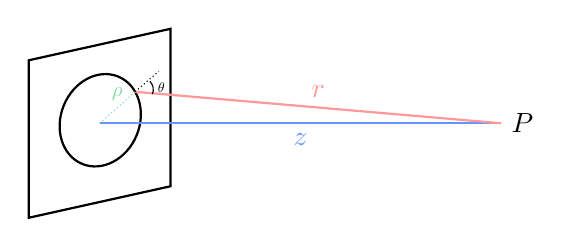
\begin{tikzpicture}
		\draw[thick] (-1,-1.2) -- (0.8,-0.8) -- (0.8,1.2) -- (-1,0.8) -- cycle;
		\draw[thick, rotate=-22.5] (-0.1,0) ellipse (0.5cm and 0.6cm);
		\draw[densely dotted,color=green!70!blue!50] (-0.1,0) -- (0.35,0.4) node[midway,above,scale=0.75] {$\rho$};
		\draw[thick,color=blue!70!cyan!60] (-0.1,0) -- (5,0) node[midway,below] {$z$} node [right]
			{\textcolor{black}{\( P \)}};
		\draw[thick,color=red!40!white] (0.35,0.4) -- (5,0) node[midway,above] {$r$};
		\draw[densely dotted] (0.35,0.4) -- (0.65,0.66);
		\draw (0.57,0.37) arc (-22.5:45:0.15cm) node[midway,right,scale=0.5] {$\theta$};
	\end{tikzpicture}
\end{center}

Assuming the point \( P \) is far enough away so that \( \theta \approx \frac{\pi}{2} \), then the \(
\mathbf{E}  \) field becomes:
\[
	\mathbf{E} = \frac{1}{4 \pi \epsilon_0 c^2}\frac{q \omega^2 x_0}{r} \cos\left[ \omega\left( t
	-\frac{r}{c} \right) \right]\hat{\boldsymbol{\theta}}
\]
Now to find the contribution due to the whole plane, we just integrate over the entire plane:
\[
	\mathbf{E} = \frac{1}{4\pi \epsilon_0 c^2}\int_\text{sheet} \frac{q \omega^2 x_0}{r}\Re\left[ e^{i \omega
	(t - r / c)} \right] 2 \pi \rho \eta \diff \rho
\]
Here, we define \( \eta \) to be the \textit{dipole density}, so the number of dipoles per unit area. We have
\( r^2 = \rho^2 + z^2 \), so \( r \diff r = \rho \diff \rho \), and hence:
\[
	\mathbf{E} = \frac{q \omega^2 x_0}{2 \epsilon_0 c^2}\int_z^{\infty} \Re\left[ e^{i \omega \left( t -
	\frac{r}{c} \right)} \right] \eta \diff r
\]
Now, if you assume that the sheet is uniform, then \( \eta = \eta_0 \), so we have:
\[
	\mathbf{E} = \frac{q \omega^2 x_0^2 \eta_0}{2 \epsilon_0c^2}\int_{z}^{\infty} \Re\left[ e^{i \omega
	\left( t - \frac{r}{c} \right)} \right] \diff r = \frac{q \omega x_0^2 \eta_0}{2 \epsilon_0 c^2}\Re\left[
\frac{c}{-i \omega} e^{ i \omega t} \left( e^{-i \omega (\infty) / c} - e^{-i \omega z / c} \right)\right]
\]
But the term in square brackets clearly diverges, so something has gone wrong here. In particular, it turns
out that our assumption that the dipole density is a constant, \( \eta = \eta_0 \), is not physical. So, we
need to "regularize" it by introducing a cutoff scale \( \Lambda \). We will do it as follows. Instead of
letting \( \eta(r) \) be a constant, we will instead define it as:
\[
	\eta(r) = \begin{cases}
		\eta_0 \left( 1 - \frac{r}{\Lambda} \right) & r < \Lambda\\
		0 & r > \Lambda
	\end{cases}
\]
It turns out that we not only need to regularize \( \eta \), but also do so in a way that is continuous. If
we were to just introduce an abrupt cutoff to \( \eta(r) \), then that discontinuity will also cause issues.
When we do this integral now, we will first assume \( \Lambda \) is finite, then take \( \Lambda \to \infty
\) after computing the integral. Now, using this refined \( \eta(r) \), we get the following result:
\begin{align*}
	\mathbf{E} &= \frac{q x_0 \omega^2 \eta_0}{2 \epsilon_0 c^2}\int_{z}^{\Lambda} 
	\Re\left[ e^{i \omega \left( t - \frac{r}{c} \right)}\left( 1 - \frac{r}{\Lambda} \right) \right] \diff r\\
			   &= \frac{\omega^2}{2 \epsilon_0 c^2} q x_0 \eta_0 \Re\left\{e^{i \omega t}\left[ 
					   {\color{blue!80!black}{\frac{c}{-i \omega}e^{i \omega \Lambda / c}}} - \frac{c}{-i
						   \omega} e^{-i \omega z / c} + 
						   {\color{blue!80!black}{\frac{c}{i \omega} e^{- i \omega \Lambda / c}}} 
						   - \frac{c}{i \omega}\frac{z}{\Lambda} e^{-i \omega z / c}
						   - \frac{c}{\omega^2} \frac{1}{ \Lambda} e^{-i \omega \Lambda / c} 
				   + \frac{c^2}{\omega^2}\frac{1}{\Lambda} e^{-i \omega z / c} 
		   \right] \right\} 
\end{align*}
Now, taking \( \Lambda \to \infty \), all \( \frac{1}{\Lambda} \) terms die off, and the two blue terms
cancel each other. So, we end up getting the result:
\[
	\mathbf{E} = \frac{\omega^2}{2 \epsilon_0 c^2}qx_0 \eta_0 \Re\left[ \frac{c}{i \omega} e^{i \omega \left(
	t - \frac{z}{c}\right)} \right] = \frac{\omega}{2 \epsilon_0 c}q x_0 \eta_0 \sin\left[ \omega\left( t -
\frac{z}{c} \right) \right]
\]
Then, remembering that \( x(t) = x_0 \cos(\omega t) \), then \( v(t) = -x_0 \omega \sin(\omega t) \), so:
\[
	\mathbf{E} = -\frac{q \eta_0}{2 \epsilon_0 c }v\left( t - \frac{r}{c} \right)
\]
And that's all we have for now. One thing you may have noticed in this integral is that the \( \Lambda \)
term didn't actually end up mattering -- we could have chosen the cutoff to be any number, and it would have
disappeared just the same. We will see why this is the case on Friday.    

 
  

	\section{February 7}
Last time, we left off after computing the integral for \( \mathbf{E} \), and we found that \( \Lambda \)
doesn't matter since it got canceled out after the computation. Now, we will discuss why this is true.      
Recall that the integral we wanted to compute was
\[
	\int_{z}^{\infty} e^{-i \omega r / c }\diff r
\]
First, let's define \( \theta = \frac{\omega}{r} \), so \( d\theta = \frac{\omega}{c}\diff r \), and our
integral becomes:
\[
	\int_{\theta_0}^{\infty}e^{-i \theta} \frac{c}{\omega} \diff \theta
\]
This integral lends itself to a very nice intuition: we can think of it as just adding up a bunch of complex
numbers together. Adding complex numbers in the complex plane can be thought of as vector addition, so
computing the integral is the same as adding up the vectors in the following diagram:

\begin{center}
	\begin{tikzpicture}
    \draw[thick,color=gray!70] (-1,-1.12) circle (1.5cm);
    \filldraw[white] (0,-1) -- (0,0) -- (1,0) -- (1,-1) -- cycle;
    \draw[color=orange!70!white] (0.2,0) arc (0:-52.12:0.2cm) node[midway,right,yshift=-0.05cm,scale=0.5] {$\theta_0$};
    \draw[thick,stealth-stealth] (0,-3) -- (0,3);
    \draw[thick,stealth-stealth] (-4,0) -- (4,0);
    \draw[thick, color=orange!70!white,-stealth] (0,0) -- (0.35,-0.45) node[right,yshift=0.1cm,scale=0.5] {$e^{-i\theta_0\left(\frac{c}{\omega}d\theta\right)}$};
    \draw[densely dotted] (0.35,-0.45) -- (0.6,-0.77);
    \draw (0.475,-0.61) arc (-52.12:-74.74:0.2cm) node[right,scale=0.35,yshift=-0.1cm] {$d\theta$};
    \draw[thick,color=blue!60!cyan!80,-stealth] (0.35,-0.45) -- (0.5,-1) node[right,scale=0.5] {$e^{-i(\theta_0+d\theta)\left(\frac{c}{\omega}d\theta\right)}$};
\end{tikzpicture}
\end{center}

Essentially, we start with a vector at an angle \( \theta_0 \), then we continually add vectors of the same
"length" together, all the while changing the angle slightly by \( d\theta \). If we continue this process,
we eventually loop back around to the origin. What this ultimately means is that when we integrate from \(
\theta_0 \) to infinity, we end up traversing this loop infinitely many times, which is why the integral
diverges. 

Now, when we add a \( \Lambda \) term, what happens is that the "length" of the vector we add each time
decreases, so instead of the addition coming out to a circle, it ends up as a \textit{spiral}. Further, if \(
\eta(\theta)\) decreases slowly enough (so make \( \Lambda \) sufficiently large, but not infinite), then the
integral will converge at the \textit{center} of the earlier circle. So, the integral looks something like
the following diagram:

\begin{center}
	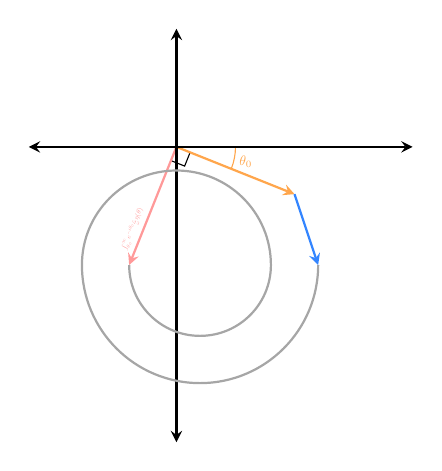
\begin{tikzpicture}[scale=1.5]
    \draw[rotate=-21.8] (0.125,0) -- (0.125,-0.125) -- (0,-0.125);
    \draw[thick,red!40!white,-stealth] (0,0) -- (-0.4,-1) node[midway,left,scale=0.25,rotate=68,yshift=0.5cm,xshift=-0.2cm] {$\int_{\theta_0}^{\infty}e^{-i\theta_0}\frac{c}{\omega}\eta(\theta)$};
    \draw[thick,orange!70!white,-stealth] (0,0) -- (1,-0.4);
    \draw[color=orange!70!white] (0.5,0) arc (0:-21.8:0.5cm) node[midway,right,yshift=-0.05cm,scale=0.5] {$\theta_0$};
    \draw[thick,color=blue!60!cyan!80,-stealth] (1,-0.4) -- (1.2,-1);
    \draw[thick,stealth-stealth] (0,-2.5) -- (0,1);
    \draw[thick,stealth-stealth] (-1.25,0) -- (2,0);
    \draw[thick, color=gray!70] (-0.4,-1) arc (-180:0:0.6cm) arc (0:180:0.8cm) arc (-180:0:1cm);
\end{tikzpicture}
\end{center}


What does the integral converge to? From the geometry, the resulting vector is perpendicular to the initial
vector, so we have:
\[
	\int_{\theta_0}^{\infty} e^{-i \theta} \frac{c}{\omega}\eta(\theta) = Re^{-i (\theta_0 + \pi / 2)}
\]
To find the radius \( R \), we also use geometry, to get \( R \diff \theta = \frac{c}{\omega} \diff \theta
\), so we get \( R = \frac{c}{\omega} \). This now explains why \( \Lambda \) doesn't matter, since whatever
value of \( \Lambda \) chosen, we will converge to the center of the circle. So, the integral becomes:
\[
	\int_{z}^{\infty}e^{-i \omega r / c} \diff r = \int_{\theta_0}^{\infty}e^{-i \theta}\frac{c}{\omega}
	\diff \theta = R e^{-i \left( \theta_0 + \frac{\pi}{2} \right)} = \frac{c}{\omega}(-i) e^{-i \omega z / c}
\]
So now applying this to the integral for \( \mathbf{E} \), we get the result from last lecture:
\[
	\mathbf{E} = \frac{q \omega x_0 \eta_0}{2 \epsilon_0 c^2} \Re\left[ \frac{c}{i} e^{i \omega \left( t -
	\frac{z}{c} \right)} \right]
\]
\subsection{The "Delayed" Wave}
Now, let's consider the following system, with a source which emits an electric field \(
\mathbf{E}_\text{source} \) and a point \( P \) far away, and we place a thin sheet of linear media in
between the two. The sheet has thickness \( \Delta z \). Phenomenologically, we know that light travels
slower in glass compared to vacuum, by a ratio of \( v = \frac{c}{n} \), so the wave will take extra time to
arrive at \( P \). In particular, the extra time is given by:
\[
	\Delta t = \frac{\Delta z}{v} - \frac{\Delta z}{c} = (n - 1) \frac{\Delta z}{c}
\]
So, with the glass in between, we have to add this \( \Delta t \) term into the exponential, and
thus:\footnote{We are being a bit lazy with the notation here, \( \mathbf{E} \) should be a vector quantity
but we only care about its magnitude for now so we'll treat it as a scalar.}
\[
	E(t, z) = E_0 e^{i \omega\left( t - \Delta t - \frac{z}{c} \right)} = E_0 e^{i \omega \left( t - \frac{n
	- 1}{c} \Delta z - \frac{z}{c} \right)}
\]
If the slab is assumed to be very thin, then we can extract the \( \Delta z \) term, and Taylor expand it:
\begin{align*}
	E(t, z) &= E_0 e^{-i \omega \frac{n - 1}{c} \Delta z} e^{-i \omega \left( t - \frac{z}{c} \right)}\\
	&= E_0 \left( 1 - i \frac{n - 1}{c}\Delta z \right) e^{i \omega\left(t - \frac{z}{c}\right)} \\ 
	&= E_0 e^{i \omega \left( t - \frac{z}{c} \right)} - \frac{i (n -1) \omega \Delta z}{c}E_0 e^{i
	\omega\left( t - \frac{z}{c} \right)}
\end{align*}
The first term can be thought of as just \( \mathbf{E}_\text{source} \), while the second term can be thought
of as the wave produced by the charges in the material.  

\subsection{A Microscopic Model}
Now, let's consider what happens in the glass itself. When a sinusoidal source electric field \(
\mathbf{E}_\text{source} = E_0 e^{i \omega t}\) contacts the glass, it will oscillate the charges inside the glass.
Microscopically, each dipole in the glass is in a potential well, which usually looks like the following:

\begin{center}
	\begin{tikzpicture}[line cap=round]
		% Axis
		\draw[thick, -latex] (-2ex,0) -- (8,0) node[below] {\( x \)};
		\draw[thick, -latex] (0,-2.5) -- (0,5) node[left] {\( U \)};	
		
		% Plot Function
		\draw[domain=0.177:7.5, samples=400, variable=\r, very thick, red] plot ({\r},{0.3/(\r*\r)-0.9/\r});
		
		% Dashed
		\draw[dashed] (2/3,0) -- +(0,-0.65) node[pos=0, above] {\( x_\text{eq} \)};
	\end{tikzpicture}
\end{center}

Here \( x_\text{eq} \) marks an equilibrium point, around which the charge oscillates. It is a (global)
minimum, so the first derivative is zero, and hence its Taylor expansion around \( x_\text{eq} \)is:
\[
	U = U(x_\text{eq}) + \frac{1}{2} U''(x_\text{eq}) (x - x_\text{eq})^2
\]
This should be somewhat familiar from classical mechanics. The equation of motion, according to 
Newton's equation, is given by:
\[
	m \ddot x = - m \omega_0^2 x + q E_0 e^{i \omega t}
\]
Intuitively, when the electric field gives the charge some energy, the charge will oscillate with a
sinusoidal motion as well, so let \( x(t) = x_0 e^{i \omega t} \). Putting this ansatz into the equation of
motion, we get:
\[
	-m \omega^2 x_0 e^{ i \omega t} = - m \omega_0^2 x_0 e^{i \omega t} + q E_0 e^{ i \omega t} \implies x_0
	= \frac{qE_0}{m(\omega_0^2 - \omega^2)}
\]
This implies that the motion for \( x(t) \) is:
\[
	x(t) = \frac{qE }{m(\omega_0^2- \omega^2)}e^{ i \omega t}
\]
Combining this result with what we have at the end of last lecture for
\( \mathbf{E} \), we have the following equation for the electric field of the dipole:
\[
	E_\text{dipole} = \Re\left[ -i \frac{q \omega}{2 \epsilon_0 c} \frac{q E_0 N \Delta z}{m(\omega_0^2 -
	\omega^2)}e^{i \omega\left( t - \frac{z}{c} \right)} \right]
\]
Here, \( N \Delta z = \eta_0 \), which is the density of charges per volume.  


	\section{February 10}
Today, we will talk about the transmission and reflection of waves in a linear medium. We will find that all
the properties we know about reflection and transmission: Snell's law, the law of reflection, they all
follow directly from enforcing the boundary conditions given by Maxwell's equations. 

Recall Maxwell's equations in a linear medium:
\begin{align*}
	\div \mathbf{D} &=  0 \\ 
	\div \mathbf{B} &= 0 \\ 
	\curl \mathbf{E} &= -\partial \mathbf{B} \\ 
	\curl \mathbf{H} &= \partial \mathbf{D} 
\end{align*}

These equations then imply the following boundary conditions:
\begin{align}
	\epsilon_1 E_1^{\perp} &= \epsilon_2 E_2^{\perp}\label{a} \\ 
	E_1^{\parallel} &= E_2^{\parallel}\label{b} \\ 
	B_1^{\perp} &= B_2^{\perp} \label{c} \\ 
	\mu_1 B_1^{\parallel} &= \mu_2 B_2^{\parallel} \label{d}
\end{align}

This is a result of using the relations \( \mathbf{D} = \epsilon \mathbf{E} \) and \( \mathbf{B} = \mu \mathbf{H} \)
in linear media. Now, with these boundary conditions set, we are ready to consider the transmission and
reflection of waves in a linear medium.  

\subsection{Normal Incidence}
First, we will consider the case where the incident wave is perpendicular to the interface. This makes the
situation easier to analyze. Let the system be described as follows: we have an incident wave from the left,
and a plane of material at \( z = 0 \). Then, the \( \mathbf{E} \) field over all space is given by:
\[
	\mathbf{E} = \begin{cases}
		\mathbf{E}_I e^{i (k_1 z - \omega t )} + \mathbf{E}_R e^{i(-k_2 z - \omega t)} & z < 0\\
		\mathbf{E}_T e^{i (k_2 z - \omega t)} & z > 0
	\end{cases}
\]
Technically, we need to take the real part of these equations, but we're going to omit that detail for
now.\footnote{What this really means is that each bold-faced vector \( \mathbf{E} \) in this equation is a
\textit{complex-valued} vector, of which you have to take the real part to get the amplitude.}  
Before we go further, it is important to note that \( \omega \) is the same for all three terms, which we can
argue to be the case in two different ways. Firstly, if you think of the incident wave as an electric field,
then it makes sense that the response from the dipoles should also follow the same frequency. Mathematically,
we also know that \( \omega \) must be the same because when we end up matching the boundary conditions, we
end up getting an equation of the form:
\[
	\mathcal{A}e^{- i \omega_I t} + \mathcal{B} e^{-i \omega_R t} = \mathcal{C}e^{- i \omega_T t}
\]
Here, \( \mathcal{A}, \mathcal{B} \) and \( \mathcal{C} \) are arbitrary constants. 
If we want this equation to hold up for all time \( t \), then the only way is if \( \omega_I = \omega_R =
\omega_T \). Now, we begin to impose the boundary conditions. The waves here are only in the \( \hat{z} \)
direction, since \( \mathbf{E} \) and \( \mathbf{B} \) are transverse waves, so \( \mathbf{E}_I, \mathbf{E}_R
\) and \( \mathbf{E}_T  \) are all in the \( xy \) plane. This immediately means that boundary conditions
\ref{a} and \ref{c} are trivially satisfied, and hence we only care about \ref{b} and \ref{d}. Starting with
\ref{b}:
\[
	\mathbf{E}_I e^{-i \omega t} + \mathbf{E}_R e^{-i \omega t} = \mathbf{E}_T e^{- i \omega t}
\]
so this gives \( \mathbf{E}_I = \mathbf{E}_R = \mathbf{E}_T \). Similarly, we can write down equations for the
magnetic field:
\[
	\mathbf{B} = \begin{cases}
		\mathbf{B}_I e^{i (k_1z - \omega t)} + \mathbf{B}_R e^{i(k_1 z - \omega t)} & z < 0 \\
		\mathbf{B}_T = e^{i(k_2 z - \omega t)} & z > 0
	\end{cases}
\]
Boundary condition \ref{d} then says:
\[
	\frac{1}{\mu_1} (\mathbf{B}_I + \mathbf{B}_R) = \frac{1}{\mu_2} \mathbf{B}_T
\]
We know that the \( \mathbf{B} \) field travels in the \( z \) direction, so using equation \ref{B-wave}, we
can write:
\[
	\mathbf{\hat{z}} \times \mathbf{E}_1 - \mathbf{\hat{z}} \times \mathbf{E}_R = \beta
	\mathbf{\hat{z}} \times \mathbf{E}_T
\]
We absorb all the constants into \( \beta = \frac{\mu_1v_1}{\mu_2v_2} \). Without loss of generality, we can
also suppose \( \mathbf{E} \) aligns in the \( \mathbf{\hat{x}} \) direction, so then we can write:
\begin{align*}
	\mathbf{E}_R &= E_R \mathbf{\hat{n}}_R = E_R (\cos \theta_R \mathbf{\hat{x}} + \sin \theta_r
	\mathbf{\hat{y}}) \\
	\mathbf{E}_T &= E_T \mathbf{\hat{n}}_T = E_T\left( \cos \theta_T \mathbf{\hat{x}} + \sin \theta_T
	\hat{\mathbf{y}} \right)
\end{align*}

Then, the \( y \)-component of boundary condition \ref{b} gives \( E_R \sin \theta_R = E_T \sin \theta_T \),
whereas the \( x \)-component of boundary condition \ref{d} gives \( E_R \sin \theta_R = -\beta E_T \sin
\theta_T \). These two equations must simultaneously be true, and since \( \beta >0 \), this forces \(
\theta_R = \theta_T = 0 \). So, we find that the reflected and transmitted waves have the same polarization
as the incident wave! 

Then, comparing the \( x \)-component of \ref{b} we get \( E_I + E_R = E_T \), while the \( y \)-component of
\ref{d} gives \( E_I - E_R = \beta E_T \). Solving both equations gives:
\[
	E_T = \frac{2}{1 + \beta}E_I , \quad E_R = \frac{1-\beta}{2}E_T = \left( \frac{1 - \beta}{1 + \beta}
	\right)E_I
\]
And this solves the boundary conditions for this specific situation! To conclude this lecture, notice that
for most materials \( \mu_1 \approx \mu_2 \approx \mu_0 \), so in these cases \( \beta \approx
\frac{v_1}{v_2} \). Further, if we have a medium where \( v_1 > v_2 \) (for example, from air to water), then
\( \beta > 1 \), so the reflected wave is written as:
\[
	\mathbf{E}_R = - \left| \frac{1 - \beta}{1 + \beta} \right|\quad \mathbf{E}_I = \left| \frac{1 - \beta}{1 +
	\beta} \right|e^{ i \pi} \left(E_1 e^{i \delta_I}\right) 
	= \left| \frac{1- \beta}{1 + \beta} \right|E_I e^{i(\delta_I
	+ \pi)}
\]
 This result actually is the motivation for why we say that the reflected wave has a \( \pi \) phase shift
 relative to the incident wave, and all we needed to do was solve some boundary conditions to get it!  
 





	\section{February 12}
Last time, we derived the intensity of \( E_R \) and \( E_T \) in terms of \( E_I \), where we have:
\[
	E_R = \left( \frac{1 - \beta}{ 1 + \beta} \right)E_I \quad E_T = \frac{2}{1 + \beta}E_I
\]
Now, recall that since \( \mathbf{S} = \frac{1}{\mu}\mathbf{E} \times \mathbf{B} \), then in a linear medium,
because of equation \ref{B-wave}, we can rewrite this as \( \mathbf{S} = \frac{1}{v}\mathbf{E} \times
(\frac{1}{v} \mathbf{k}\times \mathbf{E}) \), so the time average of \( \mathbf{S} \) is written as:
\[
	\mean{\mathbf{S}} = \frac{E^2}{\mu v} \mean{\cos^2(kz - \omega t)} = \frac{E^2}{2 \mu v} \propto E^2
\]
So, the average reflection, which is denoted as:
\[
	R \equiv \frac{\mean{\mathbf{S}_R}}{\mean{\mathbf{S}_I}} = \frac{\frac{1}{2 \mu_1 v_1}
	|E_R|^2}{\frac{1}{2\mu_1v_1}|E_I|^2} = \left( \frac{1 - \beta}{1 + \beta} \right)^2
\]
Since \( \mu_1 \approx \mu_2 \) for most materials, then \( \beta \approx \frac{v_1}{v_2} \), so most of the
time, 
\[
	R = \left(\frac{v_2 - v_1}{v_2 + v_1}\right)
\]
Similarly, we have a transmission coefficient
\[
	T \equiv \frac{\frac{1}{2\mu_2v_2}|E_T|^2}{\frac{1}{2\mu_1v_1}|E_I|^2} \approx \frac{v_1}{v_2}\left(
	\frac{2}{1 + \beta} \right)^2 = \frac{4v_1v_2}{(v_1 + v_2)^2}
\]
And as a sanity check, we should get \( R + T = 1 \) because of energy conservation, which is exactly what
we have:
\[
	R + T = \frac{(v_2 - v_1)^2}{(v_2 + v_1)^2} + \frac{4v_2v_1}{(v_1 + v_2)} = 1
\]
This, above all else, gives us confidence that the math carried out properly.  

\subsection{Oblique Incidence}
Now, we will consider the more general case, where the incident wave is no longer perpendicular to the
boundary. Here, we will see that a simple application of boundary conditions leads to fundamental laws of
reflection and refraction. Consider the following case of oblique incidence:
\begin{center}
	\begin{tikzpicture}[decoration = {markings, mark=at position 0.5 with {\arrow{>}}}]
		\draw[dashed, -stealth] (-3, 0) -- (3, 0) node[right] {\( z \)};
		\draw[-stealth] (0, -2) -- (0, 2) node[above] {\( x \)};
		\draw[cyan, postaction=decorate] (-2, -1) -- node[midway, below right] {\( \mathbf{k}_I \)} (0, 0); 
		\draw[red, postaction=decorate] (0, 0) -- node[midway, above right] {\( \mathbf{k}_R \)} (-2, 1.5);
		\draw[orange, postaction=decorate] (0, 0) --node[midway, above left] {\( \mathbf{k}_T \)} (3, 0.5);
	\end{tikzpicture}
\end{center}
the laws of optics don't change when we have oblique incidence, so we will still impose the boundary
condition that the transition is continuous. Therefore, we should expect the equations on both sides of \( z
= 0\) to match. Just like the perpendicular incidence, when we match the boundary condition at \( z = 0 \) we
will get equations of the form:
\[
	\left( \phantom{aa} \right) e^{i \mathbf{k}_I \cdot \mathbf{r}}\eval_{z =0} + 
	\left( \phantom{aa} \right) e^{i \mathbf{k}_R \cdot
	\mathbf{r}}\eval_{z = 0} = \left( \phantom{aa} \right)e^{i \mathbf{k}_T \cdot \mathbf{r} }\eval_{z = 0}
\]
For this equation to be true for all \( t \), then we require that we have the same dependence in the \( xy
\) plane for all three terms. This implies the conditions:
\begin{equation}
	\label{11:k-condition}
	(\mathbf{k}_I)_x x + (\mathbf{k}_I)_y y = (\mathbf{k}_R)_x x + (\mathbf{k}_R)_y y = (\mathbf{k}_T)_x x +
	(\mathbf{k}_T)_y y
\end{equation}
Now, without loss of generality, we can choose \( \mathbf{k}_I \) to lie in the \( xz \) plane only, so \(
(\mathbf{k}_I)_y = 0 \). But this must mean that the \( y \) component for the other two terms is also zero!
Therefore, all the rays lie in the same plane, and therefore our original diagram is accurate.

Further, this also means that from \ref{11:k-condition} we get that \( (\mathbf{k}_I)_x = (\mathbf{k}_I)_y =
(\mathbf{k}_I)_z \), and hence:
\[
	\mathbf{k}_I \sin \theta_I = \mathbf{k}_R \sin \theta_R = \mathbf{k}_T \sin \theta_T
\]
But since \( |\mathbf{k}_I| = |\mathbf{k}_R| \) as they travel through the same medium, then the only
conclusion is that \( \theta_I = \theta_R \), which is the reflection rule. The other condition we then
becomes 
\[
	\frac{\omega_1}{v_1}\sin \theta_I = \frac{\omega}{v_2}\sin \theta_T \implies \frac{1}{v_1} \sin \theta_I
	= \frac{1}{v_2} \sin \theta_T
\]
Given that \( n = \frac{c}{v} \), then we can manipulate this further to get:
\[
	n_1 \sin \theta_I = n_2 \sin \theta_T
\]
which is Snell's law! 

\subsection{Polarized Light}
Now, we will consider the case where the light is polarized. First, we will consider light that is polarized
in the plane of incidence (the case perpendicular will be left as homework):

\begin{center}
	\begin{tikzpicture}[decoration = {markings, mark=at position 0.5 with {\arrow{>}}}]
		\draw[dashed, -stealth] (-4, 0) -- (4, 0) node[right] {\( z \)};
		\draw[-stealth] (0, -2) -- (0, 2) node[above] {\( x \)};
		\draw[cyan, postaction=decorate] (-2.5, -1.25) -- node[midway, below right] {\( \mathbf{k}_I \)} (0, 0); 
		\draw[red, postaction=decorate] (0, 0) -- node[midway, above right] {\( \mathbf{k}_R \)} (-2.5, 1.25);
		\draw[orange, postaction=decorate] (0, 0) --node[midway, above left] {\( \mathbf{k}_T \)} (3, 0.5);
		\draw (2.3, 0) arc [start angle = 0, end angle = 9, radius = 2.3] 
			node[midway, right] {\( \theta_\text{out} \)};
		\draw (-1, 0) arc [start angle = 180, end angle = 205, radius = 1] node[midway, left] {\(
			\theta_\text{in} \)};
		\draw (-1, 0) arc [start angle = 180, end angle = 155, radius = 1] node[midway, left] {\(
			\theta_\text{in} \)};
		\draw[-stealth]  (-2, -1) -- (-2.15, -0.75) node[above left] {\( \mathbf{E}_I \)};
		\draw[red!40!white, -stealth]  (-2, 1) -- (-1.9, 2) node[above] {\( \mathbf{E}_R \)};
		\draw[red!40!white, dashed] (-2, 1) -- (-1.5, 2);
		\draw[red!40!white] (-1.75, 1.5) arc [start angle = 70, end angle = 93, radius = 0.5];
		\draw[red!40!white] (-1.8, 1.7) node {\scalebox{.4}{\( \phi_R \)}};
		\draw[blue!40!white, -stealth] (2, 0.33) -- (2.2, 1) node[above] {\( E_T \)};
		\draw[blue!40!white, dashed] (2, 0.33) -- (1.85, 1.23);
		\draw[blue!40!white] (1.95, 0.65) arc [start angle = 100, end angle = 82, radius = 0.5];
		\draw[blue!40!white] (2.03, 0.85) node {\scalebox{.4}{\( \phi_T \)}};
	\end{tikzpicture}
\end{center}
To begin, we will consider the most general case, so we do not assume here that \( \mathbf{E}_T \) and \(
\mathbf{E}_R \) lie in the plane of incidence. This is why we have the \( \phi_T \) and \( \phi_R \) angles.
The boundary conditions don't change despite this though, and applying them here gives us:
\begin{align}
	\label{11:cond1}\epsilon_1(\mathbf{E}_I + \mathbf{E}_R)_z &= \epsilon_2 (\mathbf{E}_T)_z\\
	\label{11:cond2}(\mathbf{E}_I + \mathbf{E}_R)_{x, y} &= (\mathbf{E}_T)_{x, y} \\ 
	\label{11:cond3}(\mathbf{B}_I + \mathbf{B}_R)_z &= (\mathbf{B}_T)_z\\
	\label{11:cond4}\frac{1}{\mu_1}(\mathbf{B}_I + \mathbf{B}_r)_{x, y} &=  \frac{1}{\mu_2}(\mathbf{B}_T)_z 
\end{align}
From the vector decomposition, we can also get these relations (check these yourself on your own time): 
\begin{align*}
	\mathbf{E}_I &= - \mathbf{E}_I \sin \theta_\text{in} \mathbf{\hat{z}} + \mathbf{E}_I \cos
	\theta_\text{in}\mathbf{\hat{x}}\\
	\mathbf{E}_R &= \mathbf{E}_R \left[ \cos \phi_R \sin \theta_\text{in}\mathbf{\hat{z}} + \cos \phi_R \cos
	\theta_\text{in} \mathbf{\hat{y}} + \sin \phi_R \mathbf{\hat{y}}\right]\\
	\mathbf{E}_T &= \mathbf{E}_T \left[ -\cos \phi_T \sin \theta_\text{out} \mathbf{\hat{z}} + \cos \phi_T
	\cos \theta_\text{out} \mathbf{\hat{x}} + \sin \phi_R \mathbf{\hat{y}} \right] 
\end{align*}
Combining the vector decomposition and the boundary conditions, we get the following set of equations:
\begin{align}
	\text{(\ref{11:cond1}):} \quad & \epsilon_1 \sin \theta_\text{in}(E_I + E_R \cos \phi_R) = \epsilon_2 \sin
	\theta_\text{out}(-E_T \cos \phi_T)\\
	\label{11:cond5} \text{(\ref{11:cond2}):} \quad & \begin{cases}
		\cos \theta_\text{in}(E_I + E_R \cos \phi_R) = \cos \theta_\text{out} (E_T \cos \phi_T)\\
		E_R \sin \phi_R = E_T \sin \phi_T \\ 
	\end{cases}\\
	\text{(\ref{11:cond3}):} \quad & \frac{E_R}{v_1} \sin \phi_k \sin \theta_\text{in} = \frac{E_T}{v_2}\sin \theta_T
	\sin \theta_\text{out}\\
	\label{11:cond6} \text{(\ref{11:cond4}):} \quad & \begin{cases}
		\frac{E_R}{v_1}\cos \theta_\text{in} \sin \phi_R = - \frac{E_T}{\mu_2v_2} \cos \theta_\text{out} \sin
		\theta_T\\
		\frac{1}{\mu_1v_1}(E_I - E_R \cos \phi_R) = \frac{1}{\mu_2v_2} E_T \cos \phi_T
	\end{cases}
\end{align}

Combining the second part of \ref{11:cond5} with the first part of \ref{11:cond6}, we can get:
\[
	E_R \sin \phi_T \cos \theta_\text{in} = -\beta E_T \sin\phi_T \cos \theta_\text{out} \implies
	\sin \phi_T(\cos \theta_\text{in} + \beta \cos \theta_\text{out}) = 0
\]
The only way this equation is true for all \( \theta_\text{in} \) is if \( \phi_T = 0 \), which then implies
that \( \phi_R = 0 \) by the second half of \ref{11:cond5}. So, what we find is that indeed \( E_R \) and \(
E_T\) do lie in the plane of incidence.  


	\section{February 14}
Last time, we showed that for waves with \( E_I \) in the incident plane, the reflected and transmitted waves
have the same polarization. That is, we found that \( \phi_R = \phi_T = 0 \). So, the six boundary conditions
we had from before now transform into:
\begin{align}
	\label{lec11:BC-1}\epsilon_1 \sin \theta_\text{in}\left( E_I - E_R \right) 
	&= \epsilon_2 \sin \theta_\text{out} E_T\\
	\label{lec11:BC-2}\cos \theta_\text{in} (E_I + E_R) &= \cos \theta_\text{out}E_T\\
	\label{lec11:BC-3}(E_I - E_R) &=  \beta E_T 
\end{align}
Reminder that \( \beta = \frac{\mu_1v_1}{\mu_2 v_2} \). Here, we see that equation \ref{lec11:BC-1} is
actually the same condition as \ref{lec11:BC-3}, but written in a different form. To see this, we have:
\[
	(E_I - E_R) = \frac{\epsilon_2 \sin \theta_\text{out}}{\epsilon_1 \sin \theta_\text{in}} E_T =
	\frac{\epsilon_2 v_2}{\epsilon_1 v_1} E_T = \frac{\mu_1v_1^2 v_2}{\mu_2v_2^2 v_1}E_T =
	\frac{\mu_1v_1}{\mu_2v_2}E_T = \beta E_T
\]
So now this means that we essentially have two boundary conditions:
\[
	E_I + E_r = \alpha E_T \quad (E_I - E_R) = \beta E_T
\]
So, we can solve for \( E_T \):
\[
	E_T = \frac{2}{\alpha + \beta} \quad E_R = \frac{\alpha - \beta}{\alpha + \beta}
\]
Now, some comments about these results. Firstly, \( E_T \) always has the same sign as \( E_I \), so this
means that the transmitted wave has no phase shift. However, depending on \( \alpha
- \beta\), the reflected wave may pick up a \( \pi \) phase shift, specifically when \( \beta > \alpha \). In
the case where we have normal incidence, then \( \alpha = 1 \), so this is why the reflected wave always
picks up a phase shift. We can also rewrite \( \alpha \):
\[
	\alpha = \frac{\cos \theta_\text{out}}{\cos \theta_\text{in}} = \frac{\sqrt{1 - \sin^2
	\theta_\text{out}}}{\cos \theta_\text{in}} = \frac{\sqrt{1 - \left( \frac{n_1}{n_2} \right)^2 \sin^2
\theta_\text{in}}}{\cos \theta_\text{in}}
\]
This results means that there is always a \( \theta_\text{in} \) such that \( \alpha - \beta = 0 \), and in
this case no reflection occurs. This \( \theta_\text{in} \) is the so-called \textbf{Brewster
angle}.\footnote{This is the reason we can attach a polarizing filter onto a camera lens and get rid of
reflections that come off the glass.}

\subsection{Brewster's Angle}
What's the explicit form of \( \theta_B	\), the critical angle? We can find \( \theta_B \) by 
setting \( \alpha = \beta \): 
\[
	\beta = \frac{\sqrt{1 - \left( \frac{n_1}{n_2} \right)^2 \sin^2 \theta_B}}{\cos \theta_B} \implies \sin^2
	\theta_B = \frac{1 - \beta^2}{\left( \frac{n_1}{n_2} \right)^2 - \beta^2 }
\]
In the case where \( \mu_2 \simeq \mu_1 \simeq \mu_0 \), then this equation becomes:
\[
	\sin^2 \theta_B = \frac{1 - \beta^2}{\frac{1}{\beta^2} - \beta^2} = \frac{\beta^2(1 - \beta^2)}{1 -
	\beta^{4}} = \frac{\beta^2}{1 + \beta^2} \implies \sin \theta_B = \frac{\beta}{\sqrt{1 + \beta^2}}
\]
We can then draw a right triangle with hypotenuse \( \sqrt{1 + \beta^2} \), which gives \( \tan \theta_B =
\frac{n_2}{n_1} \). What's the physical intuition for this phenomenon? One way you can convince yourself of
this phenomenon is to consider the microscopic picture of dipole radiation. Consider a dipole:
\begin{center}
	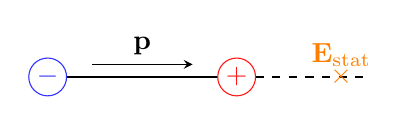
\begin{tikzpicture}[scale=0.8]
		\draw[blue!80!white] (0, 0) circle (0.3) node {\( - \)};
		\draw (0.3, 0) -- (2.7, 0);
		\draw[red!90!white] (3, 0) circle (0.3) node {\( + \)};
		\draw[dashed] (3.3, 0) -- node[pos=0.8] {\color{orange}\( \times \)} node [pos=0.8, above=0.1]
			{\color{orange} \(
			\mathbf{E}_\text{stat} \)} (5, 0); 
		\draw[-stealth] (0.7, 0.2) -- node[midway, above] {\( \mathbf{p} \)} (2.3, 0.2);
	\end{tikzpicture}
\end{center}
Now, consider the field at the point \( \mathbf{E}_\text{stat} \). The field lines can only be horizontal due
to symmetry, but this immediately means that such a field cannot be caused by a wave travelling in this
direction, since \( \mathbf{k} \perp \mathbf{E} \). Therefore, for a dipole there is no wave propagation
along the direction of the dipole moment \( \mathbf{p} \). We can also provably show this using the dipole
radiation equation, which will come in chapter 11. 

Anyways, what this means for our system is that whenever the dipoles end up oscillating in the direction that
the reflected wave would propagate in (according to the law of reflection), then there is no reflected wave.
This angle also happens to be perpendicular to \( \mathbf{k}_T \). From this observation, because \(
\mathbf{k}_T \perp \mathbf{k}_R \), then we can write: 
\[
	\theta_B + \theta_\text{out} = \frac{\pi}{2}
\]
By Snell's law, \( n_1 \sin \theta_B = n_2 \sin \theta_\text{out} = n_2 \cos \theta_B \), and indeed from
here we get the Brewster angle \( \tan \theta_B = \frac{n_2}{n_1} \). 

\subsection{Reflection and Transmission Coefficient}
Now let's go back to the diagram we made from earlier. Based on the way the waves propagate, we know that
there should be energy propagating in the \( x \) direction. By the conservation of energy, we know that \(
I_{z, \text{in}} = I_{z, \text{out}} \) along the boundary. To be specific, here \( I \) represents an
intensity, with units of energy flow per area per time. Given these units, it makes sense to use the Poynting
vector to calculate this:
\[
	|I_{z, R}| = |\mathbf{S}_R \cdot \mathbf{\hat{z}}| = \frac{E_R B_R}{\mu_1}\cos \theta_\text{in} =
	\frac{E_R^2}{\mu_1v_1} \cos \theta_\text{in}
\]
where we use the relation that \( |\mathbf{B}| = \frac{|\mathbf{E}|}{v_1} \) for waves. The incoming
intensity can also be calcualted:
\[
	|I_{z, I}| = |\mathbf{S}_I \cdot \mathbf{\hat{z}}| = \frac{E_I}{\mu_1v_1} \cos \theta_\text{in}
\]
Combining these two equations, we get:
\[
	R = \frac{|I_{z, R}|}{|I_{z, I}|} = \frac{E_R^2}{E_I^2} = \left| \frac{\alpha - \beta}{\alpha + \beta}
	\right|^2
\]
Similarly, the transmission can also be calculated as \( I_{z, T} = \frac{E_T^2}{\mu_2v_2} \cos
\theta_\text{out} \), so:
\[
	T = \frac{|I_{z, T}|}{|I_{z, I}|} = \frac{\mu_1v_1}{\mu_2v_2} \frac{|E_T|^2}{|E_I|^2}
	\frac{\cos\theta_\text{out}}{\cos\theta_\text{in}} = \alpha \beta \left( \frac{2}{\alpha + \beta}
	\right)^2
\]
Indeed, if you add these two up, you get \( R + T = 1 \), as required by conservation of energy. 

\subsection{Total Internal Reflection}

Another phenomenon that is a result of these rules is total internal reflection. This occurs when \(
\theta_\text{out} = \frac{\pi}{2} \), which gives us \( \alpha = 0 \). Looking at our formulas for \( R \)
and \( T \), this gives:
\[
	R = \left| \frac{\alpha - \beta}{\alpha + \beta} \right|^2 = 1 \quad T = \alpha \beta \left|
	\frac{2}{\alpha + \beta} \right|^2 = 0
\]
So we get no energy transmitted. What happens if we go past this critical \( \theta_c \)? Well, the effect is
that \( \sin \theta_\text{out} \) becomes imaginary. To see why, consider Snell's law:
\[
	k_I \sin \theta_I = k_T \sin \theta_T \implies \sin \theta_T = \frac{n_1}{n_2} \sin \theta_I
\]
If \( n_1 > n_2 \), then there evidently will be an angle \( \theta_I \) such that \( \sin \theta_T > 1 \),
which is not possible if we are to interpret \( \theta_T \) as an angle. One natural question one could ask
then is, instead of allowing for the possibility of \( \sin \theta_T \) to exceed 1, why not say that Snell's
law doesn't hold anymore? The reason for this is that Snell's law \textit{must} hold, as it is simply a
product of the boundary conditions imposed by Maxwell's equations. Thus, saying that Snell's law doesn't hold
is the same as saying that we violate Maxwell's equations, and of course we can't allow that. 



	\section{February 19}

Today, we will continue our discussion from last time about total internal reflection. Last time, we left off
with acknowledging that in the case where we move an angle \( \theta_I \) past the critical angle for total
internal reflection \( \theta_c \), that the \( \sin\theta_T \) term becomes imaginary. To further explore
this concept, consider now the
equations for the electric field on both sides of the medium:
\begin{align*}
	\mathbf{E} = \begin{cases}
		\Re\left\{ \tilde{\mathbf{E}}_I e^{i (\mathbf{k}_i \cdot \mathbf{r} - \omega t)} + \mathbf{E}_R
		\right\}e^{i(\mathbf{k}_R \cdot \mathbf{r} - \omega t)} & z < 0\\
		\Re\left\{ \tilde{\mathbf{E}}_{T} e^{i(\mathbf{k}_T \cdot \mathbf{r} - \omega t)} \right\}
	\end{cases}
\end{align*}
In the case where we don't have total internal reflection, it was natural to write \( \mathbf{k}_T = k_T \cos
\theta_T \mathbf{\hat{z}} + k_T \sin \theta_T \mathbf{\hat{x}} \). This was natural specifically because you
could imagine decomposing the vector \( \mathbf{k}_T \) into its \( x \) and \( z \) components. Now, the
trick when \( \sin \theta_T > 1 \) is to stop treating this as a geometric picture, but instead just
interpret \( \cos \theta_T \) and \( \sin \theta_T \) as a way to parametrize \( k_T \) in terms of \(
\theta_T \). This way, this decomposition is still allowed. Thus, we can still use Snell's law:
\[
	\sin \theta_T = \frac{v_2}{v_1} \sin \theta_I
\]
Similarly, we can expand \( \cos \theta_T \):
\begin{equation}
	\label{12:cos-imaginary}
	\cos \theta_T = \sqrt{-(\sin^2 \theta_T - 1)} = i \sqrt{\left( \frac{n_1}{n_2} \sin \theta_I \right)^2 -
	1} = i \frac{1}{n_2}\sqrt{(n_1 \sin \theta_I)^2 - n_2^2}
\end{equation}
So with this parametrization, the solution in the transmitted region is now:
\begin{align}
	E_T &= \Re\left\{ \tilde{\mathbf{E}}_T e^{i ( k_T \cos \theta_T z + k_T \sin \theta_T x - \omega t)} \right\}\\
	\label{12:ET}&= \Re\left\{ \tilde{\mathbf{E}}_T e^{-\kappa z} e^{i (k_T \sin \theta_T - \omega t)} \right\} 
\end{align}
We define \( \kappa \) as: 
\[
	\kappa = \frac{k_T}{n_2}\sqrt{(n_1 \sin \theta_I) - n_2^2} = \frac{\omega}{c} \sqrt{(n_1 \sin
\theta_I)^2 - n_2^2} 
\]
the key thing to note is that in equation \ref{12:ET}, the transmitted wave is not zero, but is a wave which
decays every quickly with a factor of \( e^{-\kappa t} \). Because of this quick decay, it's sometimes called
the \textbf{evanescent wave}. This wave transfers no energy, which can be seen through the computation of \(
R \). Because \( \cos \theta_T \) is purely imaginary by equation \ref{12:cos-imaginary}, then \( \alpha \)
is also imaginary, and hence we can write \( \alpha = ia \) with \( a \in \R \). Using the formula for \( R \)
derived at the end of last lecture, 
\[
	R = \left| \frac{\alpha - \beta}{\alpha + \beta} \right|^2 = \left| \frac{-\beta + ia}{\beta + ia}
	\right|^2 = \left| \frac{\alpha^2 + \beta^2}{\alpha^2 + \beta^2} \right| = 1
\]
Because \( R = 1 \), we conclude that there is no energy transmitted. So then if there is no energy transfer,
how is the evanescent wave allowed to exist? The answer turns out to be that \textit{on average}, there is no
net energy transfer in the \( z \) direction, which matches this result.

\subsubsection{Frustrated TIR}
The evanescent wave actually allows for a phenomenon called the \textit{frustrated} total internal
reflection. This occurs when you have two prisms separated by a very small gap, and you shine a ray through:
\begin{center}
	\begin{tikzpicture}[decoration = {markings, mark=at position 0.5 with {\arrow{>}}}]
		\draw [fill=cyan!40!white] (0, 0) -- (3, 0) -- (0, 3) -- cycle;
		\draw [fill=cyan!40!white] (3.1, 0) -- (0.1, 3) -- (3, 3) -- cycle;
		\draw[red!80!white, postaction = decorate] (2.4, -0.2) -- (1.5, 1.5);
		\draw[red!80!white, postaction = decorate] (1.5, 1.5) -- (-0.2, 2.4);
	\end{tikzpicture}
\end{center}
If the gap between the two prisms is small enough (i.e. smaller than \( \kappa ^{-1} \)), then the evanescent
wave doesn't fully die off, and we will thus get a nonzero propagating wave in the second prism. This is the
same phenomenon as tunneling in QM, except this is purely classical! 

\subsection{Wave Propagating through a Conductor}
Throughout our discussion of waves, we've considered media where there are no free charges and currents, so
\( \rho_f \) and \( \mathbf{J}_f = 0 \). This is not true in conductors, where we cannot control the current
that is generated by electromagnetic fields. To begin this discussion, again recall Maxwell's equations:
\begin{align*}
	\nabla \cdot \mathbf{D} &= \rho_f\\
	\nabla \cdot \mathbf{B} &= 0\\
	\nabla \times \mathbf{E} &= -\partial_T \mathbf{B} \\ 
	\nabla \times \mathbf{H} &= \mathbf{J}_f + \partial_t \mathbf{D} 
\end{align*}
If we then allow for the assumption that we are still in a linear medium, then this implies the equations:
\begin{align*}
	\nabla \cdot \mathbf{E} &= \frac{\rho_f}{\epsilon} \\ 
	\nabla \cdot \mathbf{B} &=  0 \\ 
	\nabla \times \mathbf{E} &= -\partial_t \mathbf{B}\\
	\nabla \times \mathbf{B} &= \mu \mathbf{J}_f + \mu \epsilon \partial_t \mathbf{E}
\end{align*}
If we are in an ohmic material, then we can use Ohm's law, \( \mathbf{J} = \sigma \mathbf{E} \), so then the
continuity equation for \( \rho_f \) gives:
\[
	\pdv{\rho_f}{t} = - \nabla \cdot \mathbf{J}_f = -\nabla \cdot (\sigma \mathbf{E}) 
	= - \frac{\sigma}{\epsilon} \rho_f
\]
This differential admits real solutions, specifically of the form: 
\[
	\rho_f(\mathbf{r}, t) = \rho(\mathbf{r}, 0) e^{- \sigma / \epsilon t}
\]
So this means that the free charges will eventually die out given long enough time. For our purposes, we will
work under this assumption. In particular, we will assume that the period of the EM waves in our systems are
much longer than the characteristic, essentially giving the free charges enough time to die out. This
translates to the conditions \( T \gg \frac{\epsilon}{\sigma} \) or \( \omega \ll \frac{\sigma}{\epsilon} \). 

 






	\section{February 21}
\subsection{EM Waves in a Conductor}
Last time we started our discussion of EM waves in a conductor, we will continue that discussion today.
Recall that we said we wanted \( \rho_f = 0 \), so Maxwell's equations read:
\begin{align*}
	\nabla \cdot \mathbf{E} &= 0 \\ 
	\nabla \cdot \mathbf{B} &= 0 \\ 
	\nabla \times \mathbf{E} &=  -\partial_t \mathbf{B} \\ 
	\nabla \times \mathbf{B} &= \mu \mathbf{J}_f + \mu \epsilon \partial_t \mathbf{E}
\end{align*}
If we further assume that our conductor is Ohmic, then \( \mathbf{J}_f = \sigma \mathbf{E} \), so taking the
curl of Faraday's law:
\begin{align*}
	\nabla \times(\nabla \times \mathbf{E}) &= -\partial_t (\nabla \times \mathbf{B})\\
	\nabla (\nabla \cdot \mathbf{E}) - \nabla^2 \mathbf{E} &= - \mu \partial_t \mathbf{J}_f + \mu \epsilon
	\partial_t^2 \mathbf{E}
\end{align*}
So rewriting this a bit, you get the following wave equation for \( \mathbf{E} \):
\begin{equation}
	\label{13:damped wave equation}
	(\nabla^2 - \mu \epsilon \partial_t^2 - \mu \sigma \partial_t) \mathbf{E} = 0
\end{equation}
Similarly, if you take the curl of the Ampere-Maxwell law, you get a similar equation for \( \mathbf{B} \):
\[
	(\nabla^2 - \mu \epsilon \partial_t^2 - \mu \sigma \partial_t) \mathbf{B} = 0
\]
Now, take a look at \ref{13:damped wave equation}. We know that we're dealing with waves, so let's have an
ansatz of \( \mathbf{E} = \mathbf{E}_0 e^{i(kz - \omega t)} \). Then, the differential equation will read:
\[
	\mu \epsilon \ddot{\mathbf{E}} = - k^2 \mathbf{E} - \mu \sigma \dot{\mathbf{E}}
\]
This is the same differential equation as that for a damped harmonic oscillator, where the \(
\dot{\mathbf{E}} \) term supplies the damping. To solve for \( \mathbf{E} \), we will consider a complex
ansatz, so \( \mathbf{E} = \mathbf{E}_0 e^{i (\tilde k z - \omega t)} \), so \( \tilde k \in \C \). Plugging
this into the equation of motion and solving for \( \tilde k \), we get:
\[
	\tilde k^2 = \mu \epsilon \omega^2\left( 1 + i \frac{\sigma}{\epsilon \omega} \right) = \left(
	\frac{\omega}{v} \right)^2 \left( 1 + i \frac{\sigma}{\epsilon \omega} \right)
\]
Now, let \( \tilde k = \frac{\omega}{v}(a + ib) \). We'll find \( a \) and \( b \) by matching coefficients.
So, we have:
\[
	\tilde k^2 = (a + ib)^2 = a^2 - b^2 + 2iab 
\]
Comparing the real and imaginary part we get \( a^2 - b^2 = 1 \) and \( 2ab = \frac{\sigma}{\epsilon \omega}
\), so solving for \( a \) and \( b \):
\begin{align*}
	a^2 - \frac{\sigma^2}{4 a^2 \epsilon^2 \omega^2} &=  1 \\ 
	a^{4} - a^2 - \frac{\sigma^2}{4 \epsilon^2 \omega^2} &=  0
\end{align*}
We can solve this with the quadratic equation:
\[
	a^2 = \frac{1 \pm \sqrt{1 + \left( \frac{\sigma}{\epsilon \omega} \right)^2}}{2}
\]
We choose the positive solution for \( a \) because \( a \in \R	\) and \( a > 0 \). Plugging this back into
\( b \), we get the combined solutions:
\[
	a = \sqrt{\frac{\sqrt{1 + \left( \frac{\sigma}{\epsilon \omega} \right)^2} + 1}{2}} \quad b =
	\sqrt{\frac{\sqrt{1 + \left( \frac{\sigma}{\epsilon \omega} \right)^2} - 1}{2}}
\]
So, if we define \( \tilde k \equiv k + i \kappa \), so \( k = \frac{\omega}{v}a \) and \( \kappa =
\frac{\omega}{v} b \), then we see that the electric field \( \mathbf{E}  \) has solutions of the form:
\[
	\mathbf{E} = \Re\left\{ \tilde{\mathbf{E}}_0 e^{-\kappa z} e^{i(kz - \omega t)} \right\}
\]
The \( e^{-\kappa z} \) term represents the fact that the waves decays as it propagates through the
conductor, eventually dying out.      

\subsection{Magnetic Phase Shift} 
In a conductor, the magnetic field propagates in the same direction as \( \mathbf{E} \), but now with a phase
shift, unlike in a vacuum. To see this, consider a magnetic field wave:
\[
	\tilde{\mathbf{B}} = \tilde{\mathbf{B}}_0 e^{i(\tilde{\mathbf{k}} \cdot \mathbf{r} - \omega t)}
\]
Here, we let \( \tilde{\mathbf{k}} = \tilde k \cdot \mathbf{\hat{k}} \). Note that this is different than the
Cartesian parametrization \( \tilde{\mathbf{k}} = \mathbf{k} + i \boldsymbol{\kappa} \), which leads to
differing mathematical results. The former is a more natural parametrization, because when we think of
travelling waves the \( \mathbf{\hat{k}} \) vector points in the direction of travel, with frequency
information encoded in the scalar \( \tilde k \). Applying Faraday's law:
\begin{align*}
	\epsilon^{ijk}\partial_j \left(E_{0k}e^{i(\tilde{\mathbf{k}} \cdot \mathbf{r} - \omega t)}\right) &=
	-\partial_t \left(B_0^{i}e^{i(\tilde{\mathbf{k}} \cdot \mathbf{r} - \omega t)}\right)\\
	\epsilon^{ijk}(i \tilde k_j) \tilde E_{0k} e^{i(\tilde{\mathbf{k}} \cdot \mathbf{r} - \omega t)} &= (i
	\omega) \tilde B_0^{i} e^{i(\tilde{\mathbf{k}} \cdot \mathbf{r} - \omega t)}\\ 
	\therefore \tilde B_0^{i} &= \epsilon^{ijk} \frac{\tilde k_j}{\omega} \tilde E_{0k}
\end{align*}
From this, we can see that the amplitude of \( B_0 \) is given by \( \tilde B_0 = (\tilde k / \omega) \tilde
E_0\). Because \( \tilde k \) is complex from the previous section, then this means we can write \( \tilde k
= \mathcal{K} e^{i \phi}\),\footnote{Note that this is still fundamentally different than letting 
	\( \tilde{\mathbf{k}} = \mathbf{k} + i \boldsymbol{\kappa} \), because here the \(
\mathcal{K} \) is a scalar, whereas in the alternative case we would need a vector.} meaning we have:
\[
	B_0 e^{i \delta_B} = \frac{\mathcal{K} e^{i \phi}}{\omega} E_0 e^{i \delta_k }
\]
Equating the two phases, we get the equation \( \delta_B = \delta_k + \phi \), implying that the \(
\mathbf{B} \) field now has a phase which causes it to lag behind the \( \mathbf{E} \) wave.  
 
% there's a small section here about K_f, should I include it? 












	\section{February 24}

\subsection{Normal Incidence on a Conductor}
Last time, we stopped by considering EM waves in a conductor, now we will consider reflection and
transmission on a conductor, in the same way we did this for linear dielectrics. Consider the following case
of an electromagnetic wave \( \mathbf{E}_I \) on the boundary between a linear dielectric and a linear
conductor.   
\begin{center}
	\begin{tikzpicture}[scale=0.5]
		\draw[-stealth] (-4, 0) -- (4, 0) node[right] {\( z \)};
		\draw[-stealth] (0, -4) -- (0, 4) node[above] {\( x \)};
		\draw[stealth-stealth, orange] (-3, -1) -- (-3, 1) node[above] {\( \mathbf{E}_I \)}; 
		\draw (-3, 4) node {linear dielectric};
		\draw (3, 4) node {linear conductor};
	\end{tikzpicture}
\end{center}
By fitting boundary conditions, we can find that the transmitted wave has the same polarization as the
incident wave, and we also have the following quantities:
\[
	\tilde \beta = \left( \frac{\mu_1v_1}{\mu_2 \omega} \right)\tilde k_2 \quad \tilde E_{0R} = \left(
	\frac{1 - \tilde \beta}{ 1+ \tilde \beta} \right)\tilde E_{0I} \quad E_{0T} = \left( \frac{2}{1 + \tilde
\beta} \right)\tilde E_{0I}
\]
Recall also our value for \( \tilde k \):
\[
	k = a + ib = \frac{\omega}{v} \left[\sqrt{\frac{\sqrt{1 + \left( \frac{\sigma}{\epsilon \omega}
		\right)^2} + 1}{2} }+ i \sqrt{\frac{\sqrt{1 + \left( \frac{\sigma}{\epsilon \omega} \right)^2} -
1}{2}}\right]
\]
Yes it's ugly, but that's what it is. Note also that for a very good conductor (that is, for \( \sigma \to
\infty \)), then \( |\tilde \beta| \to \infty \) as well. In this case, we see that the ratio 
\[
	\lim_{\tilde \beta \to \infty} \frac{1 - \tilde \beta }{1 + \tilde \beta} = -1
\]
and this means that we get \( \tilde E_{0R} = - \tilde E_{0I} \), which amounts to picking up a \( \pi \)
phase shift on reflection. Likewise, we find that \( \tilde E_{0T} \to 0 \).

\subsection{Anomalous Dispersion}
Previously, we've considered a model where we have an incident electric field \( \mathbf{E} \), which under a
roughly quadratic potential, oscillates sinusoidally. The equation of motion for such a particle is:
\[
	\ddot x = -m \omega_0^2 x + \frac{q E_0}{m}\cos(\omega t)
\]
Given this type of motion, our goal in this section is to show that the index of refraction is given by:
\[
	n = 1 + \frac{q^2 N}{2 \epsilon_0 m} \frac{1}{\omega_0^2 - \omega^2}
\]
Here \( N \) represents the number of charges per volume. This function \( n(\omega) \) explains exactly why
materials like glass bend blue light more than red light, and is the phenomenon we call \textbf{anomalous
dispersion}. This phenomenon actually has a fairly simple explanation, and it has to do with absorption and
damping. By assumption, let's add a damping term to our equation of motion:
\[
m \ddot x = - m \omega_0^2 x - m \gamma \dot x + q E_0 \cos(\omega t)
\]
And here we will solve this by considering \( x(t) = \Re(\tilde x(t)) \). We will let our ansatz be \( \tilde
x(t) = \tilde x_0 e^{-i \omega t}\), which yields the equation:
\[
	(- m \omega^2 + i m \gamma \omega + m \omega_0^2) \tilde x_0 = q E_0
\]
This leads to the equation:
\[
	\tilde x_0 = \frac{q E_0}{m(\omega_0^2 - \omega^2) - i m \gamma \omega}
\]
so we've solved for the equation of motion. Now, as the charge oscillates, we get a dipole moment:
\[
	\mathbf{p} = q \tilde x(t) = \frac{q^2}{m} \frac{1}{(\omega_0^2 - \omega^2) - i \gamma \omega} E_0 e^{-i
	\omega t}
\]
and the total polarization can be written as :
\[
	\tilde{\mathbf{P}} = \tilde{\mathbf{p}} N = \frac{q^2N}{m}\frac{1}{(\omega_0^2 0 - \omega^2) - i \gamma
	\omega} E_0 e^{-i \omega t}
\]
For a linear dielectric, we have \( \tilde{\mathbf{P}} = \epsilon \tilde \chi_e \mathbf{E} \), so using the
above equation, we can deduce the electric susceptibility:
\[
	\tilde \chi_e = \frac{q^2 N}{\epsilon_0 m}\frac{1}{(\omega_0^2 - \omega^2) - i \gamma \omega}
\]
Then, the permittivity is:
\[
	\tilde \epsilon = \epsilon_0\left( 1 + \frac{q^2 N}{\epsilon_0 m} \frac{1}{(\omega_0^2 - \omega^2) - i
	\gamma \omega} \right)
\]
Now with \( \tilde \epsilon \) solved, recall the wave equation we have when \( \mu \approx \mu_0 \) and \(
\epsilon \approx \epsilon_0 \):
\[
	(\nabla^2 - \mu \tilde \epsilon \partial_t^2) \mathbf{E} = 0
\]
Now, with the ansatz \( \tilde{\mathbf{E}} = \tilde E_0 e^{-i(\tilde k z - \omega t)} \), we get the equation
\( -\tilde k^2 + \mu \tilde \epsilon \omega^2 = 0 \) so this implies the solution:
\[
	\tilde k = \sqrt{\mu_0 \tilde \epsilon} \omega = \sqrt{\mu_0 \epsilon_0} ( 1 + \chi_e)^{1 / 2} \omega
\]
Usually, \( \tilde \chi_e \ll 1  \), so we Taylor expand here using \( (1 + x)^{n} \approx 1 + nx \).
Therefore, \( \tilde k \) becomes:
\[
	\tilde k = \sqrt{\mu_0 \epsilon_0}\left( 1 + \frac{q^2 N}{2 \epsilon_0 m}\frac{1}{(\omega_0^2 - \omega^2)
	- i \gamma \omega} \right)\omega = \sqrt{\mu_0 \epsilon_0}\left( 1 + \frac{q^2N}{2 \epsilon_0
	m}\frac{(\omega_0^2 - \omega^2) + i \gamma \omega}{\omega_0^2 - \omega^2 + \gamma^2 \omega^2} \right)
\]
This last step then allows you to think of \( \tilde k = k + i \kappa \), as you can split this into a real
and imaginary part:
\[
	\tilde k = \sqrt{\mu_0 \epsilon_0}\omega \left[ \left( 1 + \frac{q^2 N}{2 \epsilon_0 m }\frac{\omega_0^2
	- \omega^2}{(\omega_0^2 - \omega^2) + \gamma^2 \omega^2} \right) + i \left(\frac{q^2N}{2 \epsilon_0
m}\frac{\gamma \omega}{(\omega_0^2 - \omega^2) + \gamma^2 \omega^2}\right) \right]
\]
So this gives the equation: \( \tilde{\mathbf{E}} = \tilde{\mathbf{E}_0} e^{-\kappa z} e^{-i(kz - \omega t)}
\). Then, the refractive index \( n = \frac{c}{v} = \frac{c}{\omega} k \), so substituting \( k \):
\[
	n = 1 + \frac{q^2N}{2 m \epsilon_0}\frac{\omega_0^2 - \omega^2}{(\omega_0^2 + \omega^2) + \gamma ^2
	\omega^2}
\]


	\chapter{Lecture 15}

\section{Last time: Solution to electrostatic potential}

Last time, we saw that the solution to the electrostatic potential $V(r, \theta)$ assuming azimuthal symmetry
is of the form: 
\[
	V(r, \theta) = \sum_{l = 0}^\infty \left(A_lr^l + B_l \frac{1}{r^{l + 1}}\right) P_l(\cos \theta)
\] 
Let's see how this works with an example.

\begin{example*}{}{}
	Suppose we have a conductor placed in a uniform field $\vec E = E_0 \hat{z}$. We want to find the
	electrostatic
	potential everywhere in this system. 

	To start, we must first identify the boundary conditions:
	
	\begin{itemize}
		\item We expect the electric field $\vec E \to \vec E_0$ as $r \to \infty$. So, if we set $V = 0$ at $z =0$, then we get that $V \to 
	- E_0 z =-  E_0 r \cos \theta$ as $r \to \infty$. This can be shown explicitly by considering a line integral $V = \int 
	\vec E \cdot dl$, starting from $z = 0$ going to $z = z_0$ for some $z$. 
	\item We require $V = 0$ at $r \le R$, due to the properties of a conductor.  
	\end{itemize}
	Now, we are ready to impose the boundary conditions onto our general solution. Inside the sphere, we don't 
	expect $V$ to blow up, so therefore all $B_l = 0$ in the limit that $r \to \infty$. Further, since $V \to E_0 r \cos \theta$ as $r \to \
	\infty$, then we only keep the first-order $\cos \theta$ term, so we only keep $A_1 = -E_0$. Now matching
	the second boundary condition;
	\[
		A_l R^l + B_l \frac{1}{R^{l + 1}} = 0 \implies B_l = -A_l R^{2l + 1}
	\] 
	And since we know that $A_l = 0$ except $A_1$, then we only keep $B_1$ as a result. Solving, we get $B_1 = 
	E_0 R^{2l +1}$. Therefore, after matching boundary conditions we get the solution 
	\[
	V(r, \theta) = \left( -E_0 r + E_0 \frac{R^3}{r^2} \right) \cos \theta
	\] 
\end{example*}
% there is a thing about the induced charge here, but I'm not completely sure what it refers to. 

\section{Multipole Expansion}

For simplicity, let's only consider two charges $q$ placed on the $z$ axis, at a distance $d$ away from each
other. Now, we could write the potential explicitly: 
\[
 V = \frac{q}{4\pi \epsilon_0}\left( \frac{1}{\rcurs_+} - \frac{1}{\rcurs_-} \right) 
\] 
While this form is ok, we are often interested in the limit where we are very far from the source charges, 
or in other words when $\rcurs_+$ and $\rcurs_-$ are much larger than $d$. In this limit, a simplification 
can be made. First, we write
\[
\rcurs_+ = \sqrt{r^2 + \left( \frac{d}{2} \right)^2 \mp dr \cos \theta} = r\sqrt{1 \mp \frac{d}{r}\cos \theta
+ \left( \frac{d}{2r} \right)^2} 
\] 
And a similar expression for $\rcurs_-$. Therefore, 
\[
	\frac{1}{\rcurs_{\pm}} = \frac{1}{r}\left[ 1 \mp \frac{d}{r}\cos \theta + \left( \frac{d}{r} \right)^2\right]
	^{1/2} \approx \frac{1}{r}\left[ 1 \mp \left(-\frac{1}{2} \frac{d}{r} \cos \theta\right) +
	O\left( \frac{d^2}{r^2} \right)\right] \approx \frac{1}{r}\left[1 \pm \frac{d}{2r}\cos \theta\right] 
\] 
where in the last step we use the expansion $(1 + x)^n \approx 1 + nx + \dots$. Now, applying this for our 
potential, we get: 
\begin{align*}
	V = \frac{q}{4\pi \epsilon_0}\left( \frac{1}{\rcurs_+} - \frac{1}{\rcurs_-} \right) &\approx
	\frac{q}{4\pi\epsilon_0}\cdot \frac{1}{r}\left[1 + \frac{d}{2r}\cos \theta - \left( 1 - \frac{d}{2r}
	\cos \theta\right) \right]\\
	&= \frac{q}{4\pi\epsilon_0}\frac{d}{r^2}\cos \theta\\
	&= \frac{p \cos \theta}{4\pi\epsilon_0r^2}
\end{align*}
Here, we use the definition $p = qd$, where $p$ represents the \textbf{dipole moment}. We will explore more about
the dipole moment next time. 


 

	\section{February 28}
\subsection{Rectangular Wave Guide}
Now we will consider the special case where the cross section of our wave guide happens to be a perfect
rectangle. We will consider TE modes, so \( E_z = 0 \). So our objective is to solve for \( B_z \), using the
wave equation. The differential equation we want to solve is 
\[
	\left( \partial_x^2 + \partial_y^2 + \left( \frac{\omega}{c} \right)^2 - k^2 \right)B_z = 0
\]
This equation is actually solved in a very similar way to the infinite square well in quantum mechanics. We
will assume separable solutions of the form \( B_z(x,y) = X(x) Y(y) \). Then, the wave equation becomes:  
\[
	Y \partial_x^2 X + X \partial_y^2 Y + \left( \frac{\omega}{c} \right)^2 XY - k^2 XY = 0
\]
Dividing both sides by \( XY \), we get:
\[
	\frac{1}{X}\partial_x^2 X + \frac{1}{Y}\partial_y^2 Y + \left( \frac{\omega^2}{c^2} - k^2 \right) = 0
\]
Notice here that the first term only has \( x \) dependence, and the second term only has \( y \) dependence.
Therefore, for this to equal zero at all times, then we require that both these values must be constants.
Therefore, we will call:
\[
	\frac{1}{X}\partial_x^2 X = -k_x^2 \quad \frac{1}{Y}\partial_y^2 Y = -k_y^2
\]
We choose \( k_x \) and \( k_y \) such that \( k_X^2 + k_y^2 + k^2 = \left( \frac{\omega}{c} \right)^2 \).
The two separate differential equations now admit solutions of the form:
\begin{align*}
	X(x) &= A \sin (k_x x) + B \cos (k_x x) \\ 
	Y(y) &= A \sin (k_y y) + B \cos (k_y y)
\end{align*}
Now, we impose the boundary conditions: \( \tilde E_{\parallel} = 0 \) and \( \tilde B_{\perp} =
0 \). Since 
\[
	B_x = \frac{i}{\left( \frac{\omega}{c} \right)^2 - k^2}\left[ k \partial_x B_z -
	\frac{\omega}{c^2}\partial_y E_z \right]
\]
and \( E_z = 0 \) because of TE waves, then we have \( \partial_x B_z\eval_{x = 0, a} = 0 \) as a result. The
boundary conditions come down to \( \partial_x X \eval_{x = 0, a} = 0 \), which gives the condition:
\[
	k_xa = m \pi \implies k_x = \frac{m\pi}{a}
\]
Similarly, we can get \( k_y = \frac{n\pi}{b} \). 

\subsection{Cutoff Frequency}
With the differential equation solved, the equation for \( \mathbf{B} \) is now: 
\[
	\tilde B(x, y) = B_0 \cos\left( \frac{m \pi x}{a} \right) \cos\left( \frac{n \pi y}{b} \right)
\]
We also have the constraint \( k_x^2 + k_y^2 + k^2 = \left( \frac{\omega}{c} \right)^2 \), so this means:
\[
	k = \sqrt{\left( \frac{\omega}{c} \right)^2 - \left( \frac{m\pi}{a} \right)^2 - \left( \frac{n\pi}{b}
	\right)^2}
\]
This equation has an interesting consequence: if \( \left( \frac{\omega}{c} \right)^2 < \left( \frac{m\pi}{a}
\right)^2 + \left( \frac{n\pi}{b} \right)^2 \), then \( k \) becomes imaginary, and this eventually means
that the wave now decays over time, and you won't get a propagating wave. So this means that there is a
minimum frequency below which you can't get a propagating wave, which is given by the cutoff frequency
\[
	\omega_{mn} = c \pi \sqrt{\left( \frac{m}{a} \right)^2 + \left( \frac{n}{b} \right)^2}
\]
\subsection{Phase Velocity}
In a wave guide, it is possible for the phase velocity to exceed the group velocity. Consider a wave with
angular velocity \( k = \frac{1}{c}\sqrt{\omega^2 - \omega_{mn}^2} \). Then, the phase speed in the \( z \)
direction is given by:
\[
	v_\text{phase} = \frac{\omega}{k} = c \cdot \frac{\omega}{\sqrt{\omega^2 - \omega_{mn}^2}} > c
\]
How is this allowed behavior? The reason is because it is impossible to encode information in the phase of a
wave, and instead we encode it in the frequency, which travels at the \textit{group velocity}:
\[
	v_\text{group} = \dv{\omega}{k} = \left( \dv{k}{\omega} \right)^{-1} = c \cdot \frac{\sqrt{\omega^2 -
	\omega_{mn}^2}}{\omega} < c
\]
which is less than \( c \), so there is no violation of causality here. There is also a nice physical picture
for this result: consider a wave propagating through the wave guide, and here we will explicitly draw out the
wavefront:
\begin{center}
	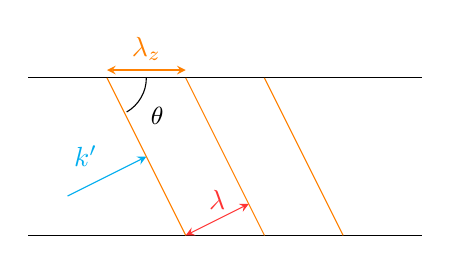
\begin{tikzpicture}
		\draw (0, 1) -- (5, 1);
		\draw (0, -1) -- (5, -1);
		\foreach \x in {1, 2, 3} {
			\draw[color=orange] (\x, 1) -- (\x+1, -1);
		}
		\draw[stealth-stealth, orange] (1, 1.1) -- node[midway, above] {\( \lambda_z \)} (2, 1.1);
		\draw[color=cyan, -stealth] (0.5, -0.5) -- node[midway, above left] {\( k' \)} (1.5, 0);
		\draw (1.5, 1) arc [radius = 0.5, start angle = 0, delta angle = -60] node[midway, below right]
			{\small \( \theta \)};
		\draw[color=red!80!white, stealth-stealth] (2, -1) -- node[midway, above] {\( \lambda \)} (2.8, -0.6); 
	\end{tikzpicture}
\end{center}
The actual wavelength \( \lambda \) is calculated as the perpendicular distance between two wavefronts, so
using this definition we see that there's a pretty simple equation for \( \lambda_z \):
\[
	\lambda_z = \frac{\lambda}{\cos \theta}
\]
And because we need to form standing waves, we have \( |k'| \cos \theta = \frac{\lambda}{k} \), so:
\[
	\cos \theta = \frac{k}{|k'|} = \sqrt{1 - \left( \frac{\omega_{mn}}{\omega} \right)^2}
\]
Now, the group velocity is given by how fast it travels in the \( z \) direction, so \( v_g = c \cos \theta
\), therefore we have:
\[
	v_g = c \sqrt{1 - \left( \frac{\omega_{mn}}{\omega} \right)^2}
\]
and we get the same result that the group velocity is less than \( c \). 

       




	\section{March 3}
\subsection{Coaxial Wave Guide}
Previously in our discussion of wave guides, we established that we can't have TEM modes, because the
condition of \( E_z = 0 \) and \( B_z = 0 \) meant no wave at all, since \( \nabla^2 V = 0 \) implies that
the potential is constant everywhere. Here, we will consider a case where TEM modes can exist. Consider a
situation where we have an inner and outer conductor:
\begin{center}
	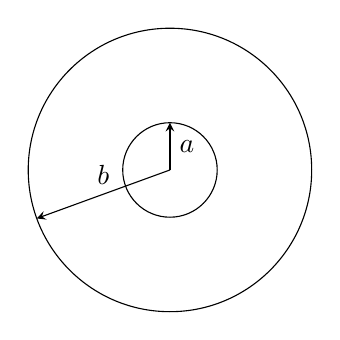
\begin{tikzpicture}[scale=0.6]
		\draw(1, 0) arc [start angle = 0, end angle = 360, radius = 1];
		\draw(3, 0) arc [start angle = 0, end angle = 360, radius = 3];
		\draw[-stealth] (0, 0) -- node[midway, right] {\( a \)} (0, 1);
		\draw[-stealth] (0, 0) -- node[midway, above] {\( b \)} (200:3);
	\end{tikzpicture}
\end{center}
To find a solution, we still use Faraday's law and Ampere-Maxwell, with the same ansatz as before: \(
\tilde{\mathbf{E}} = \tilde{\mathbf{E}}_0 (x, y) e^{i(kz - \omega t)}\), and let \( \mathbf{E}_{0z} =
\mathbf{B}_{0z} = 0 \), since we are considering TEM waves. We then get the following system of equations:
\begin{align}
	\partial_x E_y - \partial_y E_z &=  i \omega B_z & \partial_x B_y - \partial_y B_x &= -\frac{i
	\omega}{c^2} E_z \\ 
		\partial_y E_z - ik E_y &= i \omega B_x & \partial_y B_z - \partial_z B_y &= -\frac{i \omega}{c^2} E_x \\ 
		ik E_x - \partial_x E_z &= i \omega B_y & ik B_x - \partial_x B_z &= - \frac{i \omega}{c^2}E_y
\end{align}
If we now consider \( E_z = B_z = 0 \), then the equations become:
\begin{align}
	\label{17:1} 
	\partial_x E_y - \partial_y E_z &=  0 & \partial_x B_y - \partial_y B_x &= 0 \\ 
	\label{17:2}
	\partial_y E_z - ik E_y &= i \omega B_x & \partial_y B_z - \partial_z B_y &= -\frac{i \omega}{c^2} E_x \\ 
	\label{17:3}
	ik E_x - \partial_x E_z &= i \omega B_y & ik B_x - \partial_x B_z &= - \frac{i \omega}{c^2}E_y
\end{align}
Equations \ref{17:2} and \ref{17:3} look like separate equations, but they are all just saying \( \mathbf{b}
= \frac{1}{c} \mathbf{\hat{z}} \times \mathbf{E} \). Combining equation \ref{17:1} with Gauss' law, we get:
\begin{align*}
	\partial_x E_y - \partial_y E_x &= 0 & \partial_x B_y - \partial_y B_x &= 0\\
	\partial_x E_x + \partial_y E_y &= 0 & \partial_x B_x + \partial_y B_y &= 0
\end{align*}
There is no time dependence, so this is just a 2D electrostatics/magnetostatics problem. The \( \mathbf{E} \)
and \( \mathbf{B} \) field then become:
\[
	\mathbf{E}_0 = \frac{A}{s}\mathbf{\hat{s}} \quad \mathbf{B}_0 = \frac{A}{cs} \boldsymbol{\hat{\phi}}
\]
these are determined through Gauss's law and Ampere's law. Using the picture we have from above, we can then
deduce the \( \mathbf{E} \) and \( \mathbf{B} \) fields look like:

\begin{center}
	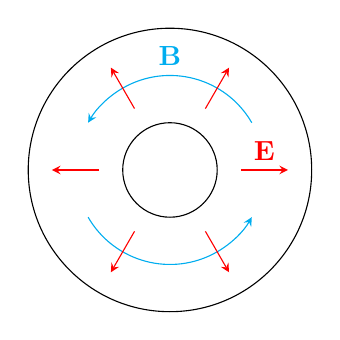
\begin{tikzpicture}[scale=0.6]
		\draw(1, 0) arc [start angle = 0, end angle = 360, radius = 1];
		\draw(3, 0) arc [start angle = 0, end angle = 360, radius = 3];
		\draw[cyan, -stealth] (30:2) arc [start angle = 30, end angle = 150, radius = 2] node[midway, above] {\(
			\mathbf{B} \)}; 
		\draw[cyan, -stealth] (210:2) arc [start angle = 210, end angle = 330, radius = 2];
		\foreach \theta in {60, 120, 180, 240, 300, 360} {
			\ifnum \theta=360 
					\draw[red, -stealth] (\theta:1.5) -- node[midway, above] {\( \mathbf{E} \)} (\theta:2.5);
			\else 
					\draw[red, -stealth] (\theta:1.5) -- (\theta:2.5);
			\fi
		};
	\end{tikzpicture}
\end{center}

\subsection{Chapter 10: Potential Formulation of EM}
Recall that in 110A, we introduced eletrostatic and magnetostatic potentials, and introduced \( \mathbf{E} =
-\nabla V\) and \( \mathbf{B} = \nabla \times \mathbf{A} \). We introduced this with the motivation that it
can simplify some problems: in the case of \( \mathbf{E} \), using \( V \) is nicer because it's a scalar
equation, but the same argument can't be said for \( \mathbf{A} \). So why did we introduce \( \mathbf{A} \),
if it is also a vector quantity? It turns out that \( \mathbf{A} \) is actually measurable effect in quantum
mechanics, through the Aharonov-Bohm effect. 

The setup is as follows: you have an electron gun, and a double slit system. We then place a solenoid that
generates a \( \mathbf{B} \) field which runs perpendicular to the direction of propagation:
\begin{center}
	\begin{tikzpicture}[scale=0.5]
		\draw[blue, -stealth] (-2, 0) -- node[midway, above] {\( e^{-} \)} (0, 0);
		\draw (3, 3) -- (3, 1);
		\draw (3, 0.5) -- (3, -0.5);
		\draw (3, -1) -- (3, -3);
		\draw (7, 3) -- (7, -3);
		\draw[red] (6, 0) arc [start angle = 0, end angle = 360, radius = 1];
		\draw[red] node at (5, 0) {\( \mathbf{B} \)};
	\end{tikzpicture}
\end{center}
In this situation, all paths that an electron can take from the source to the screen has a net \( \mathbf{B}
\) contribution of zero, but a nonzero contribution from \( \mathbf{A} \). We find that changing the \(
\mathbf{B} \) field has a \textit{measurable}, and hence \( \mathbf{A} \) is actually a measurable quantity!  


\subsection{The case for potentials}
Recall that previously, when we derived the wave equation for \( \mathbf{E} \) and \( \mathbf{B} \), we got
the equations:
\[
	(\nabla^2 - \frac{1}{c^2}\partial_t^2) \mathbf{E} = 0 \quad (\nabla^2 -
	\frac{1}{c^2}\partial_t^2)\mathbf{B} = 0
\]
And it's from these equations that we get \( c = \frac{1}{\sqrt{\mu_0 \epsilon_0}} \) to be finite. This, as
we know, means that electromagnetic waves propagate at the speed of light, but more importantly that it takes
time for them to propagate. If we now include source terms \( \rho \) and \( \mathbf{J} \), the equation
becomes: 
\begin{align*}
	(\nabla^2 - \frac{1}{c^2}\partial_t^2) \mathbf{E} &= \frac{1}{\epsilon_0}\nabla \rho + \mu_0 \partial_t
	\mathbf{J}\\
	(\nabla^2 - \frac{1}{c^2}\partial_t^2) \mathbf{B} &= -\mu_0 (\nabla \times \mathbf{J})
\end{align*}
The source terms make this wave equation very complex, since it depends on derivatives of \( \rho \) and \(
\mathbf{J} \). Its dependence on these terms also means that the solution to the \( \mathbf{E} \) field at
a time \( t \) is not simply by integrating the charge density at an earlier time -- there are velocity and
acceleration contributions that we need to consider. To fully solve the equations for 
\( \mathbf{E} \) and \( \mathbf{B} \), we use a potential-based approach. 

\subsection{\( \mathbf{E} \) and \( \mathbf{B} \) using Potentials}
From Maxwell's equations, we know that \( \nabla \cdot \mathbf{B} = 0 \), so we know that \( \mathbf{B} \)
must be divergence-less. This is consistent with our current formulation that we can express \( \mathbf{B} \)
as the curl of the magnetic potential, \( \mathbf{B} = \nabla \times \mathbf{A} \), since \( \nabla
\cdot(\nabla \times \mathbf{A}) = 0 \) for any vector potential \( \mathbf{A} \). On the other hand, we know
that \( \nabla \times \mathbf{E} = -\partial_t \mathbf{B} \), so \( \mathbf{E} \) is no longer curl-less, and
hence \( \mathbf{E} = -\nabla V	\) is no longer a sufficient equation. How should we modify our equation for
\( \mathbf{E} \) then? The solution is to "redefine" \( V \), since we can rewrite Faraday's law using \(
\mathbf{A} \):
\[
	\nabla \times \mathbf{E} = -\partial_t(\nabla \times \mathbf{A}) \implies \nabla \times (\mathbf{E} +
	\partial_t \mathbf{A}) = 0
\]
so the quantity \( \mathbf{E} + \partial_t \mathbf{A} \) instead of just \( \nabla \times \mathbf{E} \) that
is curl-less. By Helmholtz's theorem, we can then write this quantity as the gradient of some scalar function
\( V \), and hence we have:
\[
	\mathbf{E} + \partial_t \mathbf{A} = \nabla V \implies \mathbf{E} = -\nabla V - \partial_t \mathbf{A}
\]
Notice that the \( V \) is the same as the electrostatic potential we introduced earlier, but now the \(
\mathbf{E} \) field is not determined exclusively based on \( V \) but also in terms of this \( \partial_t
\mathbf{A} \) term.

So now, we can use this new \( \mathbf{E} \) to find the new form of Gauss's law fully in terms of
potentials:
\[
	\nabla \cdot (-\nabla V - \partial_t \mathbf{A}) = \frac{\rho}{\epsilon_0} \implies \nabla^2 V - \nabla
	\cdot(\partial_t \mathbf{A}) = \frac{\rho}{\epsilon_0}
\]
The Ampere-Maxwell also looks different:
\begin{align*}
	\nabla \times(\nabla \times \mathbf{A}) &= \mu_0 \mathbf{J} + \mu_0 \epsilon_0 \partial_t(-\nabla V -
	\partial_t \mathbf{A})\\
	\nabla (\nabla \cdot \mathbf{A}) - \nabla^2 \mathbf{A} &= \mu_0 \mathbf{J} - \mu_0 \epsilon_0 \partial_t
	(\nabla V) - \mu_0 \epsilon_0 \partial_t^2 \mathbf{A}\\
	(\nabla^2 \mathbf{A} - \mu_0 \epsilon_0 \partial_t^2 \mathbf{A}) - \nabla\left( \nabla \cdot \mathbf{A} +
	\mu_0 \epsilon_0 \partial_t V\right) &= -\mu_0 \mathbf{J} 
\end{align*}
And those are Maxwell's equations written purely in terms of potentials! Rewriting them slightly so that the
equations look prettier: 
\begin{align}
	\label{17:potential1}\nabla^2 V + \partial_t(\nabla \cdot \mathbf{A}) &= -\frac{\rho}{\epsilon_0} \\ 
	\label{17:potential2}
	\left( \nabla^2 - \frac{1}{c^2}\partial_t \right)\mathbf{A} - \nabla\left(\nabla \cdot \mathbf{A} +
	\frac{1}{c^2} \partial_t V\right) &= -\mu_0 \mathbf{J}
\end{align}
These two equations will be the
focus for the upcoming lectures, as we find a way to solve them. 








	\section{March 5}
Last time we left off, we derived the equations of motion for electric and magnetic potential \( V\) and 
\( \mathbf{A} \). Before we actually go ahead and solve these equations of motion, we will first talk about
gauge transformations. 


\subsection{Gauge Transformations}
To begin our discussion, let's first start by looking at the number of degrees of freedom our equations give
us. Because \( \mathbf{E} \) and \( \mathbf{B} \) are vector quantities, it would seem that we have 6 degrees
of freedom, but in reality we know from studying waves that they only have two dynamical degrees
of freedom: in the case of plane waves, we know that \( \mathbf{E} \cdot \mathbf{k} = 0 \) which knocks one
degree out, and once \( \mathbf{E} \) is determined then so is \( \mathbf{B} \) via \( \mathbf{B} =
\frac{1}{c}\mathbf{\hat{k}} \times \mathbf{E} \), so this gives only two degrees of freedom. 

Now, if you swap \( \mathbf{E} \) and \( \mathbf{B} \) out for \( V \) and \( \mathbf{A} \), it seems that
you've introduced two extra degrees of freedom: \( V \) supplies 1 and \( \mathbf{A} \) supplies the other
three. What can we do with the extra two degrees, if they cannot manifest themselves in the underlying \(
\mathbf{E} \) and \( \mathbf{B} \)? The answer is that it gives us some freedom in how we choose to define \(
V \) and \( \mathbf{A} \). 

To illustrate this point, recall that we've defined \( \mathbf{B} = \nabla \times \mathbf{A} \). Because we
know that the curl of a gradient is zero, it means that applying the transformation \( \mathbf{A} \to \mathbf{A}' +
\nabla \lambda \) doesn't affect the underlying \( \mathbf{B} \) field, since \(
\mathbf{A}' = \nabla \times \mathbf{A} + \nabla \times (\nabla \lambda) = \nabla \times \mathbf{A} \).  
The term \( \lambda \) here is called a \textbf{gauge}, and the fact that \( \mathbf{B} \) doesn't change
means that \( \mathbf{B} \) is \textbf{invariant} under this gauge. 

Now let's say that we do introduce \( \nabla \lambda \) to \( \mathbf{A} \). Then, in order to preserve the
relation \( \mathbf{E} = -\nabla V - \partial_t \mathbf{A} \), how should \( V \to V' \) transform? To figure this
out, we look at what happens when we substitute \( \mathbf{A}' \):
\[
	\mathbf{E} = -\nabla V' - \partial_t \mathbf{A}' = -\nabla V' - \partial_t (\mathbf{A} + \nabla \lambda)
	= -\nabla V - \partial_t \mathbf{A}
\]
It's clear then that in order for the equation to hold, then we require \( V' = V - \partial_t \lambda \), so
that the \( \partial_t \nabla \lambda \) terms cancel each other out. So, the full gauge transformation is:
\begin{align*}
	V & \to V' = V - \partial_t \lambda\\
	\mathbf{A} & \to \mathbf{A}' = \mathbf{A} + \nabla \lambda
\end{align*}
Now, any scalar function \( \lambda \) here will work. So, we will choose a particular \( \lambda \) that
allows \( V \) and \( \mathbf{A} \) to satisfy some additional conditions, which we can do because \( \lambda
\) does not matter. This is the process of gauge fixing: we leverage the gauge invariance to choose a \(
\lambda \) that is particularly convenient for us. 

\subsection{Coulomb Gauge}
The first gauge transformation we will look at is the \textit{Coulomb gauge}. Under this gauge, we choose \(
\lambda\) such that \( \nabla \cdot \mathbf{A} = 0 \), or in other words we choose the \( \lambda \) such
that \( \nabla^2 \lambda = - \nabla \cdot \mathbf{A} \). The equations of motion then become:
\begin{align*}
	\nabla^2 V &= -\frac{\rho}{\epsilon_0}\\
	(\nabla^2 - \frac{1}{c^2}\partial_t^2 \mathbf{A}) - \nabla\left( \frac{1}{c^2} \partial_t V \right) &=
	-\mu_0 \mathbf{J}
\end{align*}
This gauge isn't particularly useful because the equation for \( \mathbf{A} \) is still not very nice. But,
it serves as a good example to show how we actually go through the process of gauge fixing. Suppose we have
an initial potential \( \mathbf{A}' \) that has \( \nabla \cdot \mathbf{A}' \neq 0\) (for the moment I will
use the prime to denote the original and the non-primed to denote the new one after introducing the gauge).
Then, if we introduce a gauge \( \lambda \) such that \( \nabla^2 \lambda = -(\nabla \cdot \mathbf{A}') \),
the transformed potential satisfies: 
\[
	\nabla \cdot (\mathbf{A}' + \nabla \lambda) = \nabla \cdot \mathbf{A}' + \nabla^2 \lambda = 0
\]
This then implies, as we've said before, that \( \nabla^2 V = -\frac{\rho}{\epsilon_0} \). In the case where
\( \rho \neq 0 \), this \( \lambda \) is all we can do to fix the gauge -- we've run out of "extra" degrees
of freedom to introduce further gauges \( \lambda' \). However, in the case where \( \rho = 0 \), this is not
the case. We can in fact perform another gauge transformation by introducing \( \lambda' \) such that \(
\nabla^2 \lambda' = 0 \), which doesn't affect our original gauge fixing because:
\[
	\nabla \cdot (\mathbf{A} + \nabla \lambda') = \nabla \cdot \mathbf{A} + \nabla^2 \lambda' = 0
\]
so we are allowed in choosing another \( \lambda' \). Under this so-called \textit{residual} gauge
transformation, we know that
in terms of \( V \) this manifests itself as an additional \( -\partial_t \lambda' \) term, so if we set \(
\partial_t \lambda' = V \), then this gives us a final \( V \) such that \( V = 0 \).\footnote{Note that this
	\( V \) is not the original \( V \) -- it's been transformed twice, so in terms of the original \( V \)
	the equation is actually \( V \to V - \partial_t \lambda - \partial_t \lambda' \), where we set \(
\partial_t \lambda' = V - \partial_t \lambda \) to get a net zero potential.}
So now, with \( \lambda' \) we get the equations:
\[
	V = 0 \quad \nabla \cdot \mathbf{A} = 0
\]
and we've therefore reduced the original 4 degrees into two degrees of freedom, those two supplied by \(
\nabla \cdot \mathbf{A} = 0 \). Explicitly, \( \nabla \cdot \mathbf{A} = 0  \) is written as:
\[
	\partial_x A_x + \partial_y A_y + \partial_z A_z = 0
\]
We have freedom in choosing two of the three values here: suppose \( \partial_x A_x = k_x \) and \(
\partial_y A_y = k_y \), then we are forced to choose \( \partial_z A_z = -k_x - k_y\).  
 




	\section{March 7}

\question{There was an error in the lecture recording, so the notes for this lecture were pieced together
	using the provided note and lecture audio.} 

Last time, we talked about the Coulomb gauge, which gave us the equations of motion:
\begin{align*}
	\nabla^2 V &= -\frac{\rho}{\epsilon_0} \\ 
	\left( \nabla^2 - \frac{1}{c^2}\partial_t^2 \right)\mathbf{A} &= -\mu_0 \mathbf{J} + \nabla\left(
	\frac{1}{c^2}\partial_t V \right)
\end{align*}

As we've said before, the Coulomb gauge is not very useful in electrodynamics, since the time derivative
terms are quite a nightmare to deal with. What is worth commenting on is the equation for the static
potential: the fact that the equation doesn't change even when we introduce time dependence means that the
electrostatic potential can actually be measured acausally:
\[
	V(t, \mathbf{r}) = \frac{1}{4 \pi \epsilon_0} \int \frac{\rho(t', \mathbf{r}')}{\rcurs} \diff \tau'
\]
While this may be disturbing at first, it is important to note that \( V \) by itself is not measurable, and
it is instead the electric field \( \mathbf{E} \) that we measure. To that end, the electric field takes on
the form \( \mathbf{E} = -\nabla V - \partial_t \mathbf{A} \), which is not instantaneous so there is no real
causality breaking here. 

\subsection{The Lorentz Gauge}
Aside from the Coulomb gauge, we also work with the Lorentz gauge, which sets:
\begin{equation}
	\label{19:lorentz-gauge}
	\nabla \cdot \mathbf{A} + \frac{1}{c^2}\partial_t V = 0
\end{equation}
To see how this is enforced, suppose we perform the transformation \( (V, \mathbf{A}) \to (A' - \partial_t
\lambda, A' + \nabla \lambda) \). Then, in order for the above equation to hold:
\[
	\nabla(\mathbf{A}' + \nabla \lambda) + \frac{1}{c^2}\partial_t (V' - \partial_t \lambda) = \nabla \cdot
	\mathbf{A}' + \nabla^2 \lambda + \frac{1}{c^2}\partial_t V' - \frac{1}{c^2}\partial_t^2 \lambda
\]
so, enforcing \( \lambda \) to satisfy:
\[
	\left( \nabla^2 - \frac{1}{c^2}\partial_t^2 \right)\lambda = -\left( \nabla \cdot \mathbf{A}' +
	\frac{1}{c^2}\partial_t^2 V' \right)
\]
ensures that we get the desired condition. With this condition, the equation of motion now reads:
\begin{align}
	\nabla^2 V - \frac{1}{c^2}\partial_t^2 V &= -\frac{\rho}{\epsilon_0} \\ 
	\nabla^2 \mathbf{A} - \frac{1}{c^2}\partial_t^2 \mathbf{A} &= -\mu_0 \mathbf{J}
\end{align}
This is obtained by putting gauge fixing condition into equations \ref{17:potential1} and
\ref{17:potential2}. These are the wave equations for the potentials \( V \) and \( \mathbf{A} \). However,
this one gauge fixing condition doesn't completely fix the gauge. You can actually add another gauge \(
\lambda' \) while still keeping equation \ref{19:lorentz-gauge} intact, as seen below:
\[
	\nabla \cdot(\mathbf{A} + \nabla \lambda) + \frac{1}{c^2}\partial_t(V - \partial_t \lambda') = \left(
	\nabla \cdot \mathbf{A} + \frac{1}{c^2}\partial_t V\right) + \left( \nabla^2 \lambda' -
\frac{1}{c^2}\partial_t^2 \lambda'\right) = 0 
\]
so as long as we choose \( \lambda' \) such that the second term is zero, we are allowed to add this extra
gauge. The implications of this are as follows: because we modify \( V \) by adding a time derivative to \(
\partial_t \lambda' \) and we modify \( \mathbf{A} \) by adding a gradient \( \nabla \lambda \) term, it is
possible to find a \( \lambda' \) that makes both \( V - \partial_t \lambda' \) and \( A + \nabla \lambda' \)
zero. So, this means that we can always take some nonzero \( (V, \mathbf{A}) \) and use this
extra gauge symmetry to transform both fields into the zero field \( (0, \mathbf{0}) \). This reduces another
degree of freedom, and hence we are left with two, consistent with EM waves.    

\subsection{Retarded Potentials and Fields} 
The benefit of the Lorentz gauge is that it transforms the equations of motion for \( V \) and \( \mathbf{A}
\) into four copies of the same equation, named the \textbf{Klein-Gordon equation}:
\[
	\left( \nabla^2 - \frac{1}{c^2} \pdv[2]{t}\right)\phi(t, \mathbf{r}) = \rho(t, \mathbf{r})
\]
Here, \( \phi(t, \mathbf{r}) \) represents the potential and \( \rho(t, \mathbf{r}) \) is a general source
term. To solve this equation, we can use Green's functions, which first involve solving the equation using a
delta function as the source:
\[
	\left( \nabla^2 - \frac{1}{c^2}\pdv[2]{t} \right)G(t, \mathbf{r}) = \delta^{(4)}(t, \mathbf{r})
\]
Then, once the solution to \( G(t, \mathbf{r}) \) is found, we can find the general solution for \( \phi \)
by simply integrating:
\begin{equation}
	\label{19:potential}
	\phi(t, \mathbf{r}) = \int d^{4}x'\ \rho(t', \mathbf{r}') G(t - t', \mathbf{r} - \mathbf{r}')
\end{equation}
You can also check explicitly that this satisfies the Klein-Gordon equation, we'll leave that as an exercise.
The intuitive idea for why this works is that we first solve the equation for a point potential with the delta
function \( \delta^{(4)}(t, \mathbf{r}) \), which gives the contribution to the potential \( \phi \) by a
single point source at \( (t, \mathbf{r}) \). Then, we integrate over all the point sources with the
integral, which come together to give us the full equation for the potential of all sources in the system,
and that solves for the field. 

\subsection{Solving the Green's Function Equation}
One way we can solve for Green's function is to solve it in momentum space, by considering the solution to
the Fourier transform of the equation. To this end, we can write Green's function as a sum of momentum modes
\( G_k \):
\[
	G(t, \mathbf{r}) = \int d^{4}k \ G_k e^{i k \cdot x}
\]
and here we use the four-vector \( k = (k^{0}, \mathbf{k}) \) with \( k \cdot x = -k^{0}t + \mathbf{k} \cdot
\mathbf{r} \) (we use the \( (-, +, +, +) \) convention here). In momentum space, let's derive the equation
for Green's function:
\begin{align*}
	\left(\nabla^2 - \partial_t^2\right) \frac{1}{(2\pi)^{4}}\int d^{4}k \ G_k e^{i k \cdot x} 
	&= \frac{1}{(2\pi)^{4}}
	\int d^{4}k \ e^{ik \cdot x}\\
	\left(\nabla^2 - \partial_t^2\right) \int d^{4}k \ G_k e^{ik \cdot x} &= \int d^{4}k \ e^{i k \cdot x}\\
	\left(\nabla^2 - \partial_t^2\right) G_k e^{ik \cdot x} &= e^{ik \cdot x}
\end{align*}
Now let's expand the \( k \cdot x \) on the left hand side:
\[
	G_k \left( \nabla^2 - \partial_t^2 \right)e^{i(- k^{0}t + \mathbf{k} \cdot \mathbf{r}} = e^{ik \cdot x}
\]
Then, computing the derivatives, we have:
\begin{align*}
	G_k \left( (k^{0})^2 - \mathbf{k} \cdot \mathbf{k} \right)e^{i k\cdot x} &= e^{i k \cdot x}\\
	\left( (k^{0})^2 - \mathbf{k} \cdot \mathbf{k} \right)G_k &=  1 \\ 
	\therefore G_k &=  \frac{1}{\left( (k^{0})^2 - \mathbf{k} \cdot \mathbf{k} \right)} 
\end{align*}
With this, we can now write the full integral for \( G(t, \mathbf{r}) \):
\begin{equation}
	\label{19:greens-function}
	G(t, \mathbf{r}) = \frac{1}{(2\pi)^{4}} \int d^{4}k \ \frac{e^{i k \cdot x}}{\left( (k^{0})^2 -
	\mathbf{k} \cdot \mathbf{k} \right)}
\end{equation}
There are some problems with this integral though: firstly, it's not well-defined, especially when \( |k^{0}|
= \pm \sqrt{\mathbf{k}\cdot \mathbf{k}}\), which will cause the integral to blow up. Therefore, treating this
integral classically is not the right idea, and we will instead have to borrow some tools from complex
analysis.    
 
 
  





	\section{March 10}
Recall that in the last lecture, we derived the following form for the Green's function equation in momentum
space:
\[
	G(t, \mathbf{r}) = \int \frac{d^{4}k}{(2\pi)^{4}} \frac{ e^{i k\cdot x}}{(k^{0})^2 - |\mathbf{k}|^2}
\]
The denominator is troubling, because it implies that the integrand blows up to infinity when \( k^{0} =
\pm |\mathbf{k}| \), so we need to evaluate this integral using complex analysis. We will introduce all the
tools necessary for complex analysis necessary in class, so there's no need to look for outside sources.
However, for a full treatment of complex analysis (highly recommended!) you should go take a full course on
it -- there's just no way to do it justice in 3 lectures of time. With that said, let's try our best to
illustrate the main components we'll need from complex analysis.   

\subsection{Complex Analysis}
To start, let's consider the basic complex plane:
\begin{center}
	\begin{tikzpicture}
		\draw (-3, 0) -- (3, 0) node[right] {\( x = \Re(z)\)}; 
		\draw (0, -3) -- (0, 3) node[above] {\( y = \Im(z) \)};
		\draw[red!80!white, -stealth] (0, 0) -- (2, 1) node[above right] {\( z = x + iy \)};
	\end{tikzpicture}
\end{center}
A complex number can always be decomposed into its real and imaginary component, in the form \( z = x + iy
\). This can be represented in the complex plane as a point \( (x,y) \), so in this sense you can think of
the complex plane as an \textit{analogue} of \( \R^2 \), but there are key differences, as we shall see in
the coming lectures. 
We can also define the complex conjugate of \( z \) as \( z^{*} = x - iy \), where we basically flip the
imaginary component. Now, motivated by this real-imaginary decomposition, we can define a complex function \(
f : \C \to \C \) as a map that takes one complex number \( (x, y) \) and transforms it into another complex
number, written as:
\[
	f(x, y) = u(x, y) + iv(x, y)
\]
So just like we can separate complex numbers, we can separate functions too. Now, if we are to consider the
derivative of \( f(z) \):
\[
	\dv{f}{z}\eval_{z_0}
\]
This is not always uniquely defined in the complex plane. The reason is because in principle there are many
different ways that you can approach \( z_0 \) in the complex plane -- from the left, right, above, etc.. So,
in order for the derivative to exist, what needs to be shown is that in \textit{all} the ways we can approach \(
z_0\), the quantity:
\[
	\lim_{\Delta z \to 0 } \frac{f(z_0 + \Delta z) - f(z_0)}{\Delta z}
\]
exists and is the same, only then can we conclude that \( f(z) \) is differentiable at \( z_0 \). Because
this is true for any \( dz \) chosen, one necessary condition for differentiability is then that the
derivative is the same when \( dz = dx \) and \( dz = i dy \). If these are equal, this means:
\begin{align*}
	\pdv{f}{x} &= \frac{1}{i}\pdv{f}{y} \\ 
	\pdv{u}{x} + i\pdv{v}{x} &= \frac{1}{i}\left( \pdv{u}{y} + i \pdv{v}{y} \right) = -i \pdv{u}{y} +
	\pdv{v}{y}
\end{align*}
Comparing the real and imaginary parts, we get the system of equations: 
\[
	\pdv{u}{x} = \pdv{v}{y} \quad \pdv{v}{x} = -\pdv{u}{y}
\]
These are canonically called the \textbf{Cauchy-Riemann Conditions}. Note also that we can express this in
terms of \( \partial_{z^{*}}f \). Recall that \( z = x + iy \) and \( z^{*} = x - iy \), so therefore:
\begin{align*}
	\pdv{z} &= \pdv{x}{z} \pdv{x} + \pdv{y}{z} \pdv{y} = \frac{1}{2}\pdv{x} + \frac{1}{2i}\pdv{y} =
	\frac{1}{2}(\partial_x - i \partial_y)\\
	\pdv{z^{*}} &= \pdv{x}{z^{*}} \pdv{x} + \pdv{y}{z^{*}} \pdv{y} = \frac{1}{2}\pdv{x} - \frac{1}{2i}\pdv{y}
	= \frac{1}{2}(\partial_x + i \partial_y) 
\end{align*}
Therefore, applying \( \partial_z^{*} f \):
\[
	\partial_{z^{*}}f = \frac{1}{2}\left( \partial_x + i \partial_y \right)f = \frac{1}{2}(\partial_x u -
	\partial_y v) + \frac{i}{2}\left( \partial_x v + \partial_y u \right) 
\]
The terms in both parentheses are the Cauchy-Riemann conditions, so the Cauchy-Riemann conditions are
equivalent to saying that \( \partial_{z^{*}}f = 0 \). It turns out that the C-R conditions, along with a
constraint on continuity also provides a \textit{sufficient} condition on differentiability, which we
summarize in the theorem below:
\begin{theorem}[Differentiability]
	A function \( f(z) = u(x, y) + i v(x, y) \) is differentiable in a region of the complex plane if and
	only if the Cauchy-Riemann conditions are satisfied, and all first partial derivatives of \( u \) and \(
	v \) are continuous in that region. 	
\end{theorem}
\begin{definition}[Analyticity] 
	A function \( f: \C \to \C \) is \textit{analytic} at a point \( z_0 \) if it is differentiable at \( z_0
	\) and all other points in some neighborhood of \( z_0 \). 
\end{definition}
\subsection{Integrals of Complex Functions}
Now let's consider integrating a function \( f = u + iv \) along a path \( \mathcal{P} \):
\[
	\int_{\mathcal{P}} f \diff z = \int_{\mathcal{P}} (u + iv) (dx + i \diff y) = \int_{\mathcal{P}}(u \diff
	x - v \diff y) + i\int_{\mathcal{P}} (v \diff x + u \diff y)
\]
Written this way, it is reasonable to think of integrating \( f \) as taking the line integral over a path \(
P\) of two real vector fields \( A_1(u, -v) \) and \( A_2(v, u) \): 
\[
	\int_{\mathcal{P}}f \diff z = \int_{\mathcal{P}}\mathbf{A}_1 \cdot \diff \mathbf{r} + i \int_{\mathcal{P}}
	\mathbf{A}_2 \cdot \diff \mathbf{r}
\]
Now borrowing from multivariable calculus, we know that these integrals are path independent if the vector
functions \( \mathbf{A}_1 \) and \( \mathbf{A}_2 \) have zero curl. But, looking at the conditions for
\( \mathbf{A}_1 \) and \( \mathbf{A}_2 \) to be curl-less:
\begin{align*}
	\nabla \times \mathbf{A}_1 &= \partial_x \mathbf{A}_{1y} - \partial_y \mathbf{A}_{1x} = -\partial_x v -
	\partial_y u\\
	\nabla \times \mathbf{A}_2 &= \partial_x \mathbf{A}_{2y} - \partial_y \mathbf{A}_{2x} 
	= \partial_x u - \partial_y v 
\end{align*}
These are exactly the Cauchy-Riemann conditions! So, if a function is analytic along all points in a path \(
\mathcal{P}\), the resulting integral is path independent. We can extend this even further, by saying that if
\( f(z) \) is analytic on a closed contour \( \mathcal{C} \) and all points inside the region bounded by \(
\mathcal{C} \), then:
\[
	\oint_{\mathcal{C}}f(z) \diff z = 0
\]
The point about \( f(z) \) needing to be analytic on all points within \( \mathcal{C} \) is a detail that
needs further elaboration. What if \( f(z) \) has a singularity inside \( \mathcal{C} \)? Suppose \( f \)
does have a singularity at \( z_0 \). Then, we can expand \( f \) as:
\[
	f = \sum_{n = -\infty}^{\infty} a_n (z - z_0)^{n} = \dots + \frac{a_{-2}}{(z - z_0)^2} + \frac{a_{-1}}{z
	- z_0} + a_0 + a_1 (z - z_0) + \dots 
\]
Now, if we consider a circular contour \( \mathcal{C} \) centered at \( z_0 \) with a radius of \( R \):

\begin{center}
	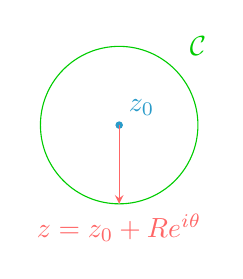
\begin{tikzpicture}[scale=2]
		\filldraw[cyan!80!black] (0, 0) circle (0.02) node [above right] {\( z_0 \)};
		\draw[green!80!black] (0, 0) circle (0.5);
		\node[green!80!black] at (0.5, 0.5) {\( \mathcal{C} \)};
		\draw[red!60!white, -stealth] (0, 0) -- (270:0.5) node[below] {\( z = z_0 + Re^{i \theta} \)};
	\end{tikzpicture}
\end{center}
then we write \( z = z_0 + Re^{i \theta} \), so we re-express \( z - z_0 = Re^{i \theta} \) in the definition
for \( f \). This definition also means \( dz = d\left( Re^{i \theta} \right) =
i Re^{i \theta} \diff \theta \). So, the contour integral becomes:
\begin{align*}
	\oint_{\mathcal{C}}f \diff z &= \int_{0}^{2\pi} \left( \sum_{n = -\infty}^{\infty} a_n (Re^{i \theta})^{n}
	\right) i Re^{i \theta} \diff \theta\\
	&= \sum_{n = -\infty}^{\infty} i \int_{0}^{2\pi}R^{n + 1} a_n e^{i (n + 1) \theta}\diff \theta \\ 
	&= \sum_{n = -\infty}^{\infty} i R^{n + 1}a_n \int_{0}^{2\pi} e^{i(n + 1) \theta}\diff \theta 
\end{align*}
Now, the integral over \( \theta \) is only nonzero when \( n = -1 \), where we have \( \int_{0}^{2\pi} \diff
\theta = 2\pi\). Therefore, the integral becomes:
\[
	\oint_{\mathcal{C}} f \diff z = 2 \pi i a_{-1}
\]
This quantity is sometimes called the \textbf{residue} of \( f \) at the point \( z_0 \), which is sometimes
denoted as \( \Res[f(z_0)] \). As an aside note, in the case where \( a_m  = 0 \) for all \( m \leq -2 \),
then we can find the residue \( a_{-1} \) by using:
\[
	\Res[f(z_0)] = a_{-1} = \lim_{z \to z_0} (z - z_0) f(z)
\]
This is true because if all the terms \( m \leq -2 \) are zero, then the only factor that doesn't contain a
\( z - z_0 \) term is \( a_{-1} \), so taking the limit immediately extracts the term. 
 
 
 



	\section{March 17}
Recall that last time, we talked about analytic functions, and we said that if \( f = f(z) \) is analytic on
a contour \( \mathcal{C} \) and the region inside \( \mathcal{C} \), then \( \oint_{\mathcal{C}}f(z) \diff z
= 0 \). Then, if \( f \) has a singularity within \( \mathcal{C} \), then 
\[
	\oint_{\mathcal{C}}f\left( z \right) \diff z = 2\pi i a_{-1}
\]
where \( a_{-1} \) is the coefficient of the inverse power \( (z - z_0)^{-1} \). Now, even though in the
previous example we used the contour of a circle, we can generalize this to any contour as well. Consider the
following contour:
\begin{center}
	\begin{tikzpicture}[decoration={markings,mark=at position 0.5 with {\arrow{stealth}}}, scale = 2]
		\draw[thick,-stealth] (0,-0.25) -- (0,2) node[right] {$\mathbb{C}$};
		\draw[thick,-stealth] (-0.25,0) -- (2,0);
		\draw[thick,green!70!blue!50,fill=blue!70!cyan!60,fill opacity=0.25] (1,0.5) circle (0.75cm)
			node[below,right,yshift=-0.75cm,xshift=1.3cm,opacity=1,scale=0.75] {\( \mathcal{C}_2 \)};
		\draw[thick,green!70!blue!50,fill=white] (1,0.5) circle (0.25cm) node[above=0.1,scale=0.75]
			{\( \mathcal{C}_1 \)};
		\filldraw[white] (1.125,0.45) rectangle (2,0.55);
		\draw[thick,green!70!blue!50,postaction={decorate}] (1.228,0.55) -- (1.76175,0.55)
			node[midway,above,scale=0.5] {\( -\mathcal{P} \)};
		\draw[thick,green!70!blue!50,postaction={decorate}] (1.76175,0.45) -- (1.228,0.45)
			node[midway,below,scale=0.5] {\( \mathcal{P} \)};
		\filldraw[green!70!blue!50] (1,0.5) circle (0.025cm);
\end{tikzpicture}
\end{center}
The diagram may be hard to see, but essentially the inner circle is \( \mathcal{C}_1 \), the outer curve is
\( \mathcal{C}_2 \), and we have a path \( \mathcal{P} \) that enters and exits. Assume that we make the gap
between \( \mathcal{P} \) and \( -\mathcal{P} \) to be infinitesimally small, so that the entire integral
approximates the contour \( \mathcal{C} \) as best as possible.
Here, the enclosed region of \( \mathcal{C} \) does not enclose any singularities, so we know already that \(
\oint_{\mathcal{C}} f(z) \diff z = 0 \). Now, if we expand the left hand side:
\[
	\oint_{\mathcal{C}}f(z) \diff z = \int_{\mathcal{C}_1} f(z) \diff z + \int_{\mathcal{C}_2} f(z) \diff z +
	\int_{\mathcal{P}} f(z) \diff z + \int_{-\mathcal{P}}f(z) \diff z
\]
the integrals over \( \mathcal{P} \) and \( -\mathcal{P} \) of course cancel, so we have:
\[
	2\pi i \Res[f(z_0)] = \int_{\mathcal{C}_2}f(z) \diff z
\]
In some sense this is actually very similar to Ampere's law. Recall that Ampere's law states \( \oint
\mathbf{B} \diff \boldsymbol{\ell} = \mu_0 I_{\text{enc}} \), so if we imagine a current going in the 
\( \mathbf{\hat{z}} \) direction a loop enclosing it in the \( xy \)-plane:
\begin{center}
	\begin{tikzpicture}
		\draw(-1, 0) -- (4, 0);
		\draw(0, -1) -- (0, 4);
		\filldraw (2, 2) circle (0.02);
		\draw (2, 2) circle (0.1) node [above right] {\( I \)};
		\draw[green!80!black] (2, 2) circle (0.8);
		\node[green!80!black] at (3, 2.5) {\( \mathcal{C} \)};
	\end{tikzpicture}
\end{center}
We know from 110A that here the \( \mathbf{B} \) field from the wire can be expressed as
\[
	B = \frac{\mu_0 I}{2 \pi r}
\]
(ignoring the vector comopnent for now), so if we deifne \( \tilde I = \frac{\mu_0 I}{2\pi} \), then we write
Ampere's law in this case as
\[
	\int \mathbf{B} \diff \boldsymbol{\ell} = 2\pi \tilde I
\]
So in this sense, we can think of the current flowing perpendicular as a kind of singularity. Of course, you
could extend this argument to having multiple currents, and likewise there's nothing stopping us from doing
the same in complex analysis, so in general:
\[
	\oint_{\mathcal{C}}f(z) \diff z = \sum_n 2\pi i \Res[f(z_n)]
\]
Now, coming back to physics, remember that our goal is to solve for Green's function \( G(t, \mathbf{r}) \)
for the Klein-Gordon equation \( (\nabla^2 - \partial_t^2)G(t, \mathbf{r}) = \delta^{(4)}(t, \mathbf{r}) \).
Moreover, we showed that:
\[
	G(t, \mathbf{r}) = \int \frac{d^{4}k}{(2\pi)^{4}} \frac{e^{i (-k^{0}t + \mathbf{k} \cdot
	\mathbf{r}})}{(k^{0})^2 - |\mathbf{k}|^2}
\]
Now, we can write the denominator as a difference of squares:
\[
	G(t, \mathbf{r}) = \int \frac{d^{4}k}{(2\pi)^{4}} e^{i(-k^{0} t + \mathbf{k} \cdot \mathbf{r})} \left[
	\frac{1}{((k^{0} - |\mathbf{k}|) (k^{0} + |\mathbf{k}|)} \right]	
\]
Clearly, we have singularities at \( k^{0} = \pm |\mathbf{k}| \). Using what we've learned from complex
analysis, integrating over \( k^{0} \in \R \) is the same as integrating over \( k^{0} \in \C \), 
but integrating over the real line only. This means we take the integral:
\begin{center}
	\begin{tikzpicture}[decoration = {markings, mark=at position 0.5 with {\arrow{>}}}, scale=0.5]
		\draw (-3, 0) -- (3, 0);
		\draw (0, -3) -- (0, 3);
		\filldraw[cyan!80!black] (-1, 0) circle (0.02) node[below] {\( -|\mathbf{k}| \)};
		\filldraw[cyan!80!black] (1, 0) circle (0.02) node[below] {\( |\mathbf{k}| \)};
		\draw[green!80!black, postaction=decorate] (-3, 0) -- (-1, 0); 
		\draw[green!80!black, postaction=decorate] (1, 0) -- (3, 0);
		\draw[green!80!black, postaction=decorate] (-1, 0) -- (1, 0);
	\end{tikzpicture}
\end{center}
Clearly we can't do this immediately because of the singularities at \( \pm |\mathbf{k}| \). Further, because
the residue theorem requires a closed loop, we can't immediately apply that either because the line is not
closed. So, our strategy is to basically integrate over a loop still, but make the extra part we add
contribute nothing to the overall integral. We can do that as follows: for \( t > 0 \), we can use the loop:
\begin{center}
	\begin{tikzpicture}[decoration = {markings, mark=at position 0.5 with {\arrow{>}}}, scale = 0.5]
		\draw (-3, 0) -- (3, 0);
		\draw (0, -3) -- (0, 3);
		\draw[green!80!black, postaction=decorate] (-3, 0) -- (0, 0);
		\draw[green!80!black, postaction=decorate] (0, 0) -- (3, 0);
		\draw[green!80!black, postaction=decorate] (3, 0) arc [start angle = 0, end angle = -180, radius = 3];
	\end{tikzpicture}
\end{center}
The idea is basically to close the loop by using a very large semicircular arc, which can be parametrized as:
\[
	e^{-i(\Re(k^{0}) + i \Im(k^{0}))t} = e^{-i\Re(k^{0})t} e^{\Im(k^{0})t}
\]
when \( \Im(k^{0}) < 0 \) and \( t > 0 \), then the factor from this contour exponentially decays away, due
to the factor of \( e^{\Im(k^{0})t} \). So, we've successfully create a loop where the extra contribution
doesn't matter at all. Similarly, for \( t < 0 \), we can use the other half circle with the same purpose:  
\begin{center}
	\begin{tikzpicture}[decoration = {markings, mark=at position 0.5 with {\arrow{>}}}, scale = 0.5]
		\draw (-3, 0) -- (3, 0);
		\draw (0, -3) -- (0, 3);
		\draw[green!80!black, postaction=decorate] (-3, 0) -- (0, 0);
		\draw[green!80!black, postaction=decorate] (0, 0) -- (3, 0);
		\draw[green!80!black, postaction=decorate] (3, 0) arc [start angle = 0, end angle = 180, radius = 3];
	\end{tikzpicture}
\end{center}
Finally, we can deal with the singularities themselves. Because we aren't allowed to walk over them directly,
our strategy will basically be to "walk around" them:
\begin{center}
	\begin{tikzpicture}[decoration = {markings, mark=at position 0.7 with {\arrow{>}}}]
		\draw (-3, 0) -- (3, 0);
		\draw (0, -3) -- (0, 3);
		\filldraw[green!80!black] (-1, 0) circle (0.02) node[above] {\( -|\mathbf{k}| \)};
		\filldraw[green!80!black] (1, 0) circle (0.02) node[below] {\( |\mathbf{k}| \)};
		\draw[cyan!80!black, postaction=decorate] (-3, 0) -- (-1.2, 0);
		\draw[cyan!80!black, postaction=decorate] (-1.2, 0) arc [start angle = 180, end angle = 360, radius = 0.2];
		\draw[cyan!80!black, postaction=decorate] (-0.8, 0) -- (0.8, 0);
		\draw [cyan!80!black, postaction=decorate] (0.8, 0) arc [start angle = 180, end angle = 0, radius =
			0.2];
		\draw[cyan!80!black, postaction=decorate] (1.2, 0) -- (3, 0);
	\end{tikzpicture}
\end{center}
so now our integral can be decomposed into three parts: the straight parts, and the two loops, all of which
are well defined. Introducing these loops also begs another question: how should we go about choosing whether
we go above or below them? There are 4 ways in total that we can go over both singularities, so how do we
know the path we've chosen is the "correct" one? The answer to this question depends on the physics of the
system: in our case, since \( \delta^{(4)}(t, \mathbf{r}) \) has a spike at \( t = 0 \), then we expect that
for \( t < 0 \), our integral should evaluate to zero and for \( t > 0 \) we expect a nonzero contribution.
Therefore, for \( t < 0 \), we should choose a method that doesn't enclose the singularities at all.
By that same token, we should choose the contour that encloses both singularities in the \( t > 0 \) case.   


 



	\section{March 19}
Today, we will finally solve for Green's function. Last time, we talked about how the \( t < 0 \) case
integrates to zero by choosing the path that avoids both singularities, and now we choose the path that
includes both for \( t > 0 \). Recall that the integral we want to solve is:
\[
	G(t, \mathbf{r}) = \int \frac{d^{4}k}{(2\pi)^{4}} \frac{e^{i k\cdot x}}{(k^{0})^2 - |\mathbf{k}|^2}
\]
and the contour we will integrate over is:
\begin{center}
	\begin{tikzpicture}[decoration = {markings, mark=at position 0.7 with {\arrow{>}}}, scale=0.8]
		\draw (-3, 0) -- (3, 0);
		\draw (0, -3) -- (0, 3);
		\filldraw[green!80!black] (-1, 0) circle (0.02) node[below] {\( -|\mathbf{k}| \)};
		\filldraw[green!80!black] (1, 0) circle (0.02) node[below] {\( |\mathbf{k}| \)};
		\draw[cyan!80!black, postaction=decorate] (-3, 0) -- (-1.2, 0);
		\draw[cyan!80!black, postaction=decorate] (-1.2, 0) arc [start angle = 180, end angle = 0, radius = 0.2];
		\draw[cyan!80!black, postaction=decorate] (-0.8, 0) -- (0.8, 0);
		\draw [cyan!80!black, postaction=decorate] (0.8, 0) arc [start angle = 180, end angle = 0, radius =
			0.2];
		\draw[cyan!80!black, postaction=decorate] (1.2, 0) -- (3, 0);
		\draw [cyan!80!black, postaction=decorate] (3, 0) arc [start angle = 0, end angle = -180, radius =
			3];
	\end{tikzpicture}
\end{center}
Remember, we want to include both singularities so this is the only contour that we can choose. 
First, we will invoke the identity \( \frac{1}{a^2 - b^2} = \frac{1}{2b}\left[ \frac{1}{a - b} - \frac{1}{a +
b} \right] \), this will allow us to write the integrand as a Laurent series, so we can extract the \( a_{-1}
\) term directly. So the integral to solve is now:
\begin{multline*}
	\frac{1}{(2\pi)^{4}} \int d^{3}k \int dk^{0}\, e^{-i k^{0}t} e^{i \mathbf{k} \cdot \mathbf{r}}
	\frac{1}{2|\mathbf{k}|} \left[
	\frac{1}{k^{0} - |\mathbf{k}|} - \frac{1}{k^{0} + |\mathbf{k}|} \right] 
	\\= \frac{1}{(2\pi)^{4}} \int
	d^{3}k \int_{\mathcal{C}}dk^{0}\, e^{-i k^{0} t} e^{i \mathbf{k} \cdot
	\mathbf{r}}\frac{1}{2|\mathbf{k}|}\frac{1}{(k^{0} - |\mathbf{k}|)} - \frac{1}{(2\pi)^{4}}\int d^3k
	\int_{\mathcal{C}}dk^{0}\, e^{-i k^{0} t} e^{i \mathbf{k} \cdot \mathbf{r}}
	\frac{1}{2|\mathbf{k}|}\frac{1}{(k^{0} + |\mathbf{k}|)}
\end{multline*}
The residue for these two integrals can be found using the limit as \( k^{0} \to \pm |\mathbf{k}| \), so the
integral becomes:
\[
	\frac{1}{(2\pi)^{4}} \int d^3 k\,  e^{i \mathbf{k} \cdot \mathbf{r}} \frac{-2\pi i}{2|\mathbf{k}|} e^{-i
	|\mathbf{k}|t} - \frac{1}{(2\pi)^{4}} \int d^3k\,e^{i \mathbf{k} \cdot \mathbf{r}}
	\frac{1}{2|\mathbf{k}|}(-2\pi i) e^{i|\mathbf{k}|t}
\]
the negative signs in the \( (-2 \pi i) \) are there because of our choice to evaluate the integral
clockwise. Now the integral can be combined together, giving:
\[
	\frac{i}{(2\pi)^3} \int d^3k \, \frac{e^{i \mathbf{k} \cdot \mathbf{r}}\left( e^{i |\mathbf{k}|t} - e^{-i
	|\mathbf{k}|t} \right)}{2|\mathbf{k}|}
\]
WLOG, we set \( k^3 \) in the direction of \( \mathbf{\hat{r}} \) (recall, this is the vector pointing from
the origin to the source), therefore the integral becomes:
\[
	\frac{i}{(2\pi)^3}\int_{0}^{\infty} d |\mathbf{k}| |\mathbf{k}|^2 \int_{0}^{\pi} 
	\frac{e^{i |\mathbf{k}|r \cos \theta}\left( e^{i |\mathbf{k}| t} - e^{-i |\mathbf{k}|t}
	\right)}{2|\mathbf{k}|} \sin \theta \diff \theta \int_{0}^{2\pi} d\phi
\]
evaluating the \( \theta \) and \( \phi \) integrals simultaneously:
\begin{equation*}
	\frac{i}{(2\pi)^2} \int_{0}^{\infty} d |\mathbf{k}|\, |\mathbf{k}|^2 \frac{1}{i|\mathbf{k}|r}\frac{\left(
	e^{i |\mathbf{k}| r} - e^{-i |\mathbf{k}|r}\right) \left( e^{i|\mathbf{k}|t} e^{-i|\mathbf{k}|t}
	\right)}{2|\mathbf{k}|} \\
	= \frac{1}{(2\pi)^2}\frac{1}{2r} \int_{0}^{\infty}d|\mathbf{k}|\, \left[ \left(
	e^{i|\mathbf{k}|(t + r)} + e^{-i |\mathbf{k}|(t + r)}\right) - \left( e^{i|\mathbf{k}|(t - r)} +
	e^{-i|\mathbf{k}|(t - r)} \right) \right]
\end{equation*}
Now, doing a change of variables from \( |\mathbf{k}| \to -|\mathbf{k}| \) on the second term in both parenthesis 
expressions, then:
\[
	\int_{0}^{\infty} d|\mathbf{k}|\, e^{-i |\mathbf{k}|(t + r)} = \int_{0}^{-\infty}-d|\mathbf{k}|\,
	e^{i|\mathbf{k}|(t + r)} = \int_{-\infty}^{0} d|\mathbf{k}|\, e^{i|\mathbf{k}|(t + r)}
\]
This allows us to transform the integrals in both parentheses into one integral involving one integrand each,
and integrating over all space. Therefore, we have:
\[
	\frac{1}{(2\pi)^{2}}\frac{1}{2r}\left[ \int_{-\infty}^{\infty}d|\mathbf{k}|\, e^{i|\mathbf{k}|(t + r)} -
	\int_{-\infty}^{\infty} d|\mathbf{k}|\, e^{i|\mathbf{k}|(t - r)}\right] 
	= \frac{1}{4\pi r}\left( \delta(t + r) - \delta(t - r) \right) \\ 
\]
Since we only consider \( t > 0 \), then the \( \delta(t + r) \) term never matters since we never reach the
spike at \( t = -r \), so we can remove that term from the expression entirely. Thus, the solution is:
\[
	G(t, \mathbf{r}) = \begin{cases}
		-\frac{1}{4\pi r}\delta(t - r) & t > 0\\
		0 & t < 0
	\end{cases}
\]
With Green's function solved, we can now proceed to find the potentials \( \phi(t, \mathbf{r}) \) using
equation \ref{19:potential}:
\[
	V(t, \mathbf{r}) = \int d^{4}x' \, \left( -\frac{\rho(t', \mathbf{r}')}{\epsilon_0}G(t - t', r - r')
	\right) = \int d^{4}x' \left( -\frac{\rho(t', \mathbf{r}')}{\epsilon_0} \right)\left(
	-\frac{1}{4\pi}\frac{\delta(t - t' - \frac{\rcurs}{c})}{\rcurs} \right)
\]
So this gives us
\begin{equation}
	\label{22:V}
	V(t, \mathbf{r}) = \int d^3x' \, \frac{1}{4\pi \epsilon_0}\frac{\rho(t_r, \mathbf{r}')}{\rcurs}
\end{equation}
where \( t_r \equiv r - \frac{\rcurs}{c} \) is defined as the \textbf{retarded time}. This should make sense:
the potential at a given point is determined by what the source was at a prior time \( t_r \), rather than
the current time, since that would violate causality. Similarly, the magnetic potential \( \mathbf{A} \) is
now:
\begin{equation}
	\label{22:A}
	\mathbf{A}(t, \mathbf{r}) = \frac{\mu_0}{4\pi}\int d^3 x' \frac{\mathbf{J}(t_r, \mathbf{r})}{\rcurs}
\end{equation}
Finally, once we have \( \mathbf{A} \) and \( V \), the we can find \( \mathbf{E} = -\nabla V - \partial_t
\mathbf{A} \) and \( \mathbf{B} = \nabla \times \mathbf{A} \). 
 

	\section{March 21}
So far, we've solved the potential \( (V, \mathbf{A}) \) that satisfies the full equations of motion:
\begin{align*}
	\left( \nabla^2 - \frac{1}{c^2}\partial_t^2 \right)V &= -\frac{\rho}{\epsilon_0}\\
	\left( \nabla^2 - \frac{1}{c^2}\partial_t^2 \right) \mathbf{A} &= -\mu_0 \mathbf{J}
\end{align*}
and the solved potentials take the form:
\begin{align*}
	V(t, \mathbf{r}) &= \frac{1}{4\pi \epsilon_0}\int d\tau' \, \frac{\rho(t_r, \mathbf{r}')}{\rcurs} \\ 
	\mathbf{A}(t, \mathbf{r}) &= \frac{\mu_0}{4\pi}\int d\tau' \, \frac{\mathbf{J}(t_r, \mathbf{r}')}{\rcurs} 
\end{align*}
Now, we want to find a general expression for the fields \( \mathbf{E}, \mathbf{B} \). One way we can do this
is by directly using the equations \( \mathbf{E} = -\nabla V - \partial_t \mathbf{A} \) and \( \mathbf{B} =
\nabla \times \mathbf{A} \) (which is what Griffiths does), but	an alternative way to do this is to use the
Green's function approach we developed from earlier. The reason we can use this is because if we look at the
equations for \( \mathbf{E} \) and \( \mathbf{B} \):
\begin{align*}
	\left( \nabla^2 - \frac{1}{c^2}\partial_t^2 \right)\mathbf{E} &= \frac{1}{\epsilon_0}(\nabla \rho + \mu_0
	\partial_t \mathbf{J}) \\ 
	\left( \nabla^2 - \frac{1}{c^2}\partial_t^2 \right)\mathbf{B} &= -\mu_0 (\nabla \times \mathbf{J})
\end{align*}
we can see that the left hand side is a wave-like equation, so we can just treat the right hand side as our
"source terms". Using this approach, we can wirte the \( \mathbf{E} \) field as:
\begin{align*}
	\mathbf{E}(t, \mathbf{r}) &= \int d^{4}x' \, \left( \frac{1}{\epsilon_0}\nabla' \rho(t', \mathbf{r}') +
	\mu_0 \partial_t \mathbf{J}(t', \mathbf{r}') \right)\left( -\frac{1}{4\pi} \frac{\delta^{(4)}(t - t' -
	\rcurs / c)}{\rcurs} \right)\\
	&= -\frac{1}{4\pi} \int d^3x \, \left( \frac{1}{\epsilon_0}\nabla' \rho(t', \mathbf{r}') + \mu_0 \partial_t
	\mathbf{J}(t', \mathbf{r}')\right)\eval_{t = t_r} \frac{1}{\rcurs} 
\end{align*}
Note that we can't just throw in the evaluation: \( [\nabla' \rho(t', \mathbf{r}')]_{t = t_r} \neq \nabla'
\rho(t_r, \mathbf{r}') \), because \( t_r \) has \( r \)-dependence. To figure out the exact relation, we
look to the index notation:
\[
	\left[ \nabla' \rho(t_r, \mathbf{r}') = \pdv{t_r}{x^{i}} \partial_t \rho (t_r, \mathbf{r}') + \pdv{x^{i}}
	\rho(t_r, r')\right]
\]
Now, the term \( \pdv{t_r}{x^{i}} \) is:
\[
	\pdv{t_r}{x^{i}} = \partial_i' \left[ t - \frac{\sqrt{(x - x')^{k}(x - x')_k}}{c} \right] = \frac{(x -
	x)_i}{\rcurs c} = \frac{\hat{\brcurs}}{c}
\]
So finally:
\[
	\nabla' \rho(t_r, \mathbf{r}') = \frac{1}{c}\dot{\rho}(t_r, \mathbf{r}') \hat{\rcurs} + \left[ \nabla'
	\rho(t', \mathbf{r}') \right]_{t = t_r} \implies \nabla' \rho(t', \mathbf{r}')\eval_{t = t_r} = \nabla'
	\rho(t_r, \mathbf{r}') - \frac{1}{c}\dot{\rho}(t_r, \mathbf{r}') \hat{\brcurs}
\]
Putting this back into the \( \mathbf{E} \) field equation:
\begin{align*}
	\mathbf{E}(t, \mathbf{r}) &= -\frac{1}{4\pi}\int d^3x' \, \left[ \frac{1}{\epsilon_0}\nabla' \rho(t',
	\mathbf{r}') - \frac{1}{c}\dot{\rho}(t_r, \mathbf{r}') \hat{\rcurs} + \mu_0 \mathbf{J}(t_r, \mathbf{r}')
\right]\cdot \frac{1}{\rcurs} \\ 
&= \frac{1}{4\pi} \int d^3x' \, \left[ \frac{1}{\epsilon_0} \nabla' \left( \frac{1}{\rcurs} \right) \rho(t_r,
\mathbf{r}') + \frac{1}{c} \frac{\dot{\rho}(t_r, \mathbf{r}')}{\rcurs}\hat{\rcurs} - \frac{\mu_0
\mathbf{J}(t_r, \mathbf{r}')}{\rcurs}\right] \\ 
&= \frac{1}{4\pi \epsilon_0} \int d^3x' \, \left[ \frac{\rho(t_r, \mathbf{r}')}{\rcurs^2}\hat{\rcurs} 
	+ \frac{1}{c} \frac{\dot{\rho}(t_r, \mathbf{r}')}{\rcurs}\hat{\rcurs} - \frac{\mathbf{J}(t_r,
\mathbf{r}')}{c^2 \rcurs} \right]
\end{align*}
This form of \( \mathbf{E} \) is known as \textbf{Jefimenko's equations}, and is the most general
(relativistic) form for the \( \mathbf{E} \) field. Similarly, you can carry out the derivation for the \(
\mathbf{B} \) field, giving the result:
\[
	\mathbf{B} = \frac{\mu_0}{4\pi}\int d^3x' \, \left[ \frac{\mathbf{J}(t_r, \mathbf{r}')}{\rcurs^2} +
	\frac{\dot{\mathbf{J}}(t_r, \mathbf{r}')}{c \rcurs} \right] \times \hat{\brcurs}
\]
and that wraps up our discussion of \( \mathbf{E} \) and \( \mathbf{B} \). Now, our next goal for the next
few lectures is to derive the field and potential for a moving point charge, using these equations. To this
end, we will begin setting up for it now. Consider a particle moving along a path given by \( \mathbf{w}(t)
\), and let's consider the potential at some arbitrary point \( P \). One thing we will note first is that
despite the concept of retarded time, it is still impossible for the field at \( P \) at a given time \( t \)
to be caused by the signal emitted from two different points in space.  

The proof is as follows: suppose that this is possible, such as in the diagram below:

\begin{center}
	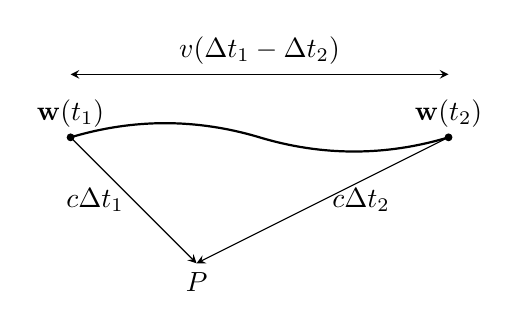
\begin{tikzpicture}[scale=0.8]

	  % Wiggly/smooth path between two nodes
	  \draw[thick] 
		(-3,0) .. controls (-2,0.3) and (-1,0.3) .. (0,0)
			   .. controls (1,-0.3) and (2,-0.3) .. (3,0);

	  % Endpoints (optional)
	  \filldraw (-3,0) circle (1.5pt) node[above] {\( \mathbf{w}(t_1) \)};
	  \filldraw (3,0) circle (1.5pt) node[above] {\( \mathbf{w}(t_2) \)};


	  \draw[-stealth] (-3, 0) -- node[midway, left] {\( c \Delta t_1 \)} (-1, -2);
	  \draw[-stealth] (3, 0) -- node[midway, right] {\( c \Delta t_2 \)} (-1, -2);
	  \node at (-1, -2.3) {\( P \)};

	  \draw[stealth-stealth] (-3, 1) -- node[midway, above] {\( v(\Delta t_1 - \Delta t_2) \)} (3, 1);
	\end{tikzpicture}	
\end{center}
If this were true, then by the triangle inequality, we'd be able to write:
\begin{align*}
	v(\Delta t_1 - \Delta t_2) + c \Delta t_2 &\geq c \Delta t_1\\
	v(\Delta t_1 - \Delta t_2) &\geq c(\Delta t_1 - \Delta t_2)\\
	\therefore v &\geq c
\end{align*}
so if this were true, we are forced to conclude that the particle travels faster than the speed of light,
which is impossible for massive particles (that is, particles having mass). 

Now, one final comment before we end today's lecture. The discussion so far with the potentials is only true
for point sources. But, now consider sources which are distributed over a non-point volume. 
Due to the retarded time, the volume we integrate over to calculate \( V(t, \mathbf{r}) \), even though we
integrate at a fixed time, is not going to be the volume over which the charge is distributed. To illustrate
this further, consider the following scenario:
\begin{center}
	\begin{tikzpicture}[decoration = snake]
 
	\node[cylinder, 
		draw = black, 
		minimum width = 1cm,
		minimum height = 2.5cm] (c) at (0,0) {};

	\node[cylinder, 
		draw = green!80!white, 
		dashed,
		minimum width = 1cm,
		minimum height = 2.5cm] (c) at (-1,0) {};

	\draw[decorate, -stealth, red!80!white] (1.2, 0) -- (1.9, 0);
	\draw[decorate, -stealth, green!80!white] (-2.1, 0) -- (-1.4, 0);
	\filldraw (4, 0) circle (1.5pt) node[right] {\( P \)};
\end{tikzpicture}
\end{center}
Suppose we want to evaluate the field at \( P \). The contribution from the front of the cylinder (red) takes a
certain time to arrive, but the back (green) takes a \textit{longer} time to cover that same distance. Therefore, the
signal measured at time \( t \) comes from the contribution of the front, and also the back but at an earlier
point in time, to compensate for that extra travel distance. So, when we integrate over the entire volume, we
aren't integrating over the charge distribution, but an extended version of the charge distribution to
account for the time of travel. We will continue this discussion next lecture.






	\section{March 31}

\subsection{The Potential of a Moving Point Charge}
Last time, we derived the equation for the potential:
\[
	V(t, \mathbf{r}) = \frac{1}{4 \pi \epsilon_0} \int d^3x \, \frac{\rho(t_r, \mathbf{r}')}{\rcurs}
\]
and we left off with the observation that if we are integrating over a moving \textit{volume}, then
the effective volume we integrate over is not \( \rho \) at a fixed time, since the signal from different
points within \( \rho \) take differing amounts of time to reach the point \( P \). Explicitly, this is
encoded in the \( t_r \) dependence of \( \rho \), since \( t_r = t - \frac{\rcurs}{c} \) means that \( t_r
\) will be different at different \( \rcurs \). 
 
Again, let's remind ourselves of the setup, and also label some lengths in the diagram:
\begin{center}
	\begin{tikzpicture}[decoration = snake]
 
	\node[cylinder, 
		draw = black, 
		minimum width = 1cm,
		minimum height = 2.5cm] (c) at (0,0) {};

	\node[cylinder, 
		draw = green!80!white, 
		dashed,
		minimum width = 1cm,
		minimum height = 2.5cm] (c) at (-1,0) {};

	\draw[decorate, -stealth, red!80!white] (1.2, 0) -- (1.9, 0);
	\draw[decorate, -stealth, green!80!white] (-2.1, 0) -- (-1.4, 0);
	\filldraw (4, 0) circle (1.5pt) node[right] {\( P \)};
	
	\draw[stealth-stealth] (-1.1, -0.8) -- node[midway, below] {\( dL \)} (1.2, -0.8);
	\draw[stealth-stealth, green!80!white] (-2.1, -0.8) -- node[midway, below] {\( v \delta t \)} (-1.1, -0.8);
	\draw[stealth-stealth, orange] (-2.1, 0.8) -- node[midway, above] {\( \widetilde{dL} \)} (1.2, 0.8);
	
\end{tikzpicture}
\end{center}
From the diagram, we can derive a relation between \( dL \) and \( \widetilde{dL} \):
\[
	v \delta t + dL = \widetilde{dL} = c \delta t
\]
The \( c \delta t \) refers to the distance travelled by the signal from the back of the cylinder in the time
it took the whole volume to move a length \( v \delta t \). Then, we can now solve for \( \tilde{dL} \):
\[
	\widetilde{dL} = \left( \frac{c}{c - v} \right)dL
\]
As-is, this equation is still not complete. We are missing the fact that this only holds if \( P \) is
directly in the direction of \( \mathbf{v} \), so more generally, we need to extract the component of the
velocity that points toward \( P \):
\[
	\widetilde{dL} = \left( \frac{c}{c - \hat{\rcurs} \cdot \mathbf{v}} \right) dL
\]
And if we regard a point charge as a really really small volume, we can use this integral to derive the
potential of a point charge. Ordinarily, we know that the integral alone would evaluate to \( q \) in the
stationary case (since we just set \( \rho = q \delta^{(3)}(\rcurs) \)); 
here it's basically the same story except now we scale by the \( \frac{c}{c - \hat{\rcurs}
\cdot \mathbf{v}} \) factor because of the length scaling:
\begin{equation}
	\label{24:V}
	V(t, \mathbf{r}) = \frac{1}{4\pi \epsilon_0}\int \frac{\rho(t_r, \mathbf{r}')}{\rcurs} \, d^3x =
	\frac{1}{4\pi \epsilon_0}\frac{qc}{\rcurs(c - \hat{\rcurs} \cdot \mathbf{v})}
\end{equation}
Although this approach gets the correct result, it should be a bit unsatisfying given that we got here by
approximating a point charge as having a tiny volume. There is a more satisfying way to arrive at this
result, using Green's functions. Suppose the point charge is given by \( \mathbf{w}(t) \), then we write the
charge density as \( \rho(\mathbf{r}) = \delta^{(3)}(\mathbf{r} - \mathbf{w}) \). Using this as our source,
then we have:
\begin{align*}
	V(t, \mathbf{r}) &= -\frac{1}{\epsilon_0} \int (c \diff t') (d^3x) \left( -\frac{1}{4\pi} \frac{\delta(c(t
	- t') - \rcurs)}{\rcurs} \right) q \delta^{(3)}(\mathbf{r}' - \mathbf{w})\\
	&= -\frac{1}{4\pi \epsilon_0}\int (c \diff t') (d^3x) \frac{\delta(ct - ct' - \rcurs)}{\rcurs}q
	\delta^{(3)}(\mathbf{r}' - \mathbf{w}(t'))
\end{align*}
One thing to note about this integral: the first delta function essentially only allows us to choose points in the
past light cone, since we only choose points where \( t' = t - \frac{\rcurs}{c} \). Now, taking the spatial
integral, we see that this effectively sets \( \mathbf{r} = \mathbf{w}(t') \) due to the second delta
function, so:
\[
	V(t, \mathbf{r}) = \int (c \diff t') \frac{\delta(ct - ct' - |\mathbf{r} - \mathbf{w}(t')|}{\rcurs}
\]
To evaluate this, recall the following relation from the delta function:
\[
	\int_{-\infty}^{\infty} \delta(f(x)) \diff x = \frac{1}{|f'(x_0)|}\int_{-\infty}^{\infty}\delta(x) \diff
	x = \frac{1}{|f'(x_0)|}
\]
In our case, we have \( f(t') = ct - ct' - \sqrt{(\mathbf{r} - \mathbf{w}(t'))(\mathbf{r} - \mathbf{w}(t'))}
\), so:
\[
	\dv{f}{t} = -c - \frac{2(\mathbf{r} - \mathbf{w}(t))\left( -\dv{\mathbf{w}}{t} \right)}{2
	\sqrt{(\mathbf{r} - \mathbf{w}(t'))(\mathbf{r} - \mathbf{w}(t'))}} = -c + \frac{\brcurs \cdot
\mathbf{v}}{\rcurs}
\]
Now, when you take the integral, we get:
\[
	V = \frac{q}{4\pi \epsilon_0} \frac{c}{\left| -c + \frac{\brcurs \cdot \mathbf{v}}{\rcurs} \right|} \cdot
	\frac{1}{\rcurs}
\]
We should be careful that in this expression \( \rcurs = \mathbf{r} - \mathbf{w}(t_r) \), so \( \rcurs \) is
evaluated at the \textit{retarded time}, not the present. Writing this result in a cleaner way, we get the
same results as before:   
\[
	V = \frac{q}{4\pi \epsilon_0} \frac{c}{(c \rcurs - \brcurs \cdot \mathbf{v})}
\]
The vector potential follows basically the same story: the integral we wish to calculate is:
\[
	A = \frac{\mu_0}{4\pi}\int d^3x \, \frac{\mathbf{J}(t_r, \mathbf{r})}{\rcurs}
\]
so for a point charge, \( \mathbf{J}(t, \mathbf{r}) = \rho v = \delta^{(3)}(\mathbf{r}' - \mathbf{w}(t'))
\mathbf{v}(t) \), so by the same argument, we have:
\[
	A = \frac{\mu_0}{4\pi}\frac{q\mathbf{v}}{\rcurs} \frac{c}{(c - \hat{\rcurs} \cdot \mathbf{v})} =
	\frac{\mu_0}{4\pi}\frac{qcv}{(c\rcurs - \brcurs \cdot \mathbf{v})} = \frac{V}{c^2} \cdot \mathbf{v}
\]
Again, here we have \( \rcurs = \mathbf{r} - \mathbf{w}(t_r) \): all the quantities here are evaluated at the
\textit{retarded time}, not at the present!
 


	\section{April 2}
Today, we're going to continue our discussion from last lecture. Recall that there, we calculated the
following equations for the fields:
\[
	V = \frac{1}{4\pi \epsilon_0} \frac{qc}{\rcurs c - \brcurs \cdot \mathbf{v}} \quad \mathbf{A} =
	\frac{\mu_0}{4\pi} \frac{qc \mathbf{v}}{c \rcurs - \rcurs \cdot \mathbf{v}}
\]
One thing to note about this equation is that the scaling factor in the denominator is \textit{not} due to
length contraction! Although they look similar in form, this factor is a result of the fact that we are no
longer integrating over the charge distribution because of its motion. With \( V \) and \( \mathbf{A} \), we
can now calculate \( \mathbf{E} \) and \( \mathbf{B} \) using the standard formulas:
\[
	\mathbf{E} = -\nabla V - \partial_t \mathbf{A} \quad \mathbf{B} = \nabla \times \mathbf{A}
\]
To begin this process, we start by calculating some gradients we will need. First up, we calculate \( \nabla
\rcurs \):
\[
	\nabla \rcurs = \partial_i \sqrt{(x_k - w_k)(x^{k} - w^{k})} = \frac{2 (x_k - w_k)(\delta_i^{k} -
	\partial_i w^{k}(t_r))}{2 \rcurs} = \frac{\brcurs}{\rcurs} - \nabla t_r(\hat{\brcurs} \cdot \mathbf{v})
\]
Now we need \( \nabla t_r \):
\[
	\nabla t_r = \partial_i \left( t - \frac{\rcurs}{c} \right) = -\frac{1}{c} \nabla \rcurs
\]
We now combine the two equations together and get:
\[
	\nabla \rcurs = \frac{c \hat{\brcurs}}{c \hat{\brcurs} - \brcurs \cdot \mathbf{v}} \quad 
	\nabla t_r = - \frac{\brcurs}{c \rcurs - \brcurs \cdot \mathbf{v}}
\] 
Next up, \( \partial_t \rcurs \):
\[
	\partial_t \rcurs = \partial_t \sqrt{\brcurs \cdot \brcurs} = \frac{2 \brcurs \cdot \partial_t \brcurs}{2
	\sqrt{\brcurs \cdot \brcurs}} = \hat{\brcurs} \cdot \partial_t (\mathbf{r} - \mathbf{w}(t)) =
	-\hat{\brcurs} \cdot \mathbf{v}(t_r) \left( \pdv{t_r}{t} \right)
\]
here we need \( \partial_t t_r \):
\[
	\partial_t t_r = \partial_t \left( t - \frac{\rcurs}{c} \right) = 1 - \frac{1}{c}\partial_t \rcurs
\]
combine again:
\[
	\partial_t \rcurs = -\frac{\hat{\brcurs} \cdot \mathbf{v}}{1 - \frac{\hat{\brcurs} \cdot \mathbf{v}}{c}}
	\quad 
	\partial_t t_r = \frac{1}{1 - \frac{\hat{\brcurs} \cdot \mathbf{v}}{c}}
\]
Now we come back to the main equation:
\[
	-\nabla V = -\partial_i \left( \frac{qc}{4\pi \epsilon_0} \frac{1}{c \rcurs - \brcurs \cdot \mathbf{v}}
	\right) = \frac{qc}{4\pi \epsilon_0} \frac{1}{(c \rcurs - \brcurs \cdot \mathbf{v})^2}\partial_i (c
	\brcurs - \brcurs\cdot \mathbf{v}) = \frac{qc}{4\pi \epsilon_0} \frac{1}{(c \rcurs - \brcurs \cdot
	\mathbf{v})^2} \left[ \frac{c^2 \brcurs}{c \rcurs - \brcurs \cdot \mathbf{v}} - (\partial_i \rcurs^{k})
	v_k - \rcurs^{k}(\partial_i v_k) \right]
\]
Notice that the gradient of the dot product is very nice in index notation -- all you have to do is use
product rule, as opposed to using the product rule given at the end of Griffiths. Now, \( \partial_i v_k(t_r)
\) is:
\[
	\partial_i v_k(t_r) = \partial_i t_r \dot{v}_k = (\partial_i t_r) a_k
\]
So now:
\[
	-\nabla V = \frac{qc}{4 \pi \epsilon_0} \frac{1}{(c \rcurs - \brcurs \cdot \mathbf{v})^2}\left[
	\frac{(c^2 - v^2) \brcurs}{c \rcurs - \brcurs \cdot \mathbf{v}} - \mathbf{v} + \frac{(\mathbf{a} \cdot
\brcurs) \brcurs}{c \rcurs - \brcurs \cdot \mathbf{v}} \right]
\]
As for \( \partial_t \mathbf{A} \):
\[
	-\partial_t \mathbf{A} = -\partial_t \left[ \frac{\mu_0}{4\pi} \frac{qc \mathbf{v}(t_r)}{c \rcurs -
	\brcurs \cdot \mathbf{v}} \right] = \frac{\mu_0 qc}{4 \pi}\left[ \frac{\mathbf{v} \partial_t (c \rcurs -
	\brcurs\cdot \mathbf{v}) - (\partial_t \mathbf{v}) (c \rcurs - \brcurs \cdot \mathbf{v})}{(c \rcurs - 
	\brcurs\cdot \mathbf{v})^2} \right] = \frac{q}{4\pi \epsilon_0} \frac{1}{(c \rcurs - \brcurs \cdot
\mathbf{v})^2} \left[ \frac{\rcurs v^2 - c \brcurs \cdot \mathbf{v} - \rcurs (\mathbf{a} \cdot \brcurs)}{c
\rcurs - \brcurs \cdot \mathbf{v}} \mathbf{v} - \rcurs \mathbf{a} \right]
\]
\question{\textbf{Author's Note:} I will admit that the algebra was done a bit more carefully in lecture than I've
	typed up here. However, I will also say that the calculations were largely uninteresting -- it's just a
bunch of chain rule so I didn't bother including it.}


	\section{April 4}
\subsection{Field of Moving Charges}
Last time, we concluded with derivation of the components to the \( \mathbf{E} \) field:   
\begin{align*}
	-\nabla V &= \frac{qc}{4 \pi \epsilon_0} \frac{1}{(c \rcurs - \brcurs \cdot \mathbf{v})^2} \left[
	\frac{(c^2 - v^2) \brcurs}{c \rcurs - \brcurs \cdot \mathbf{v}} + \frac{(\mathbf{a} \cdot \brcurs)
\brcurs}{c \rcurs - \brcurs \cdot \mathbf{v}} - \mathbf{v} \right]\\
		-\partial_t \mathbf{A} &= \frac{qc}{4\pi \epsilon_0} \frac{1}{(c \rcurs - \brcurs \cdot \mathbf{v})^2}
	\left[ \frac{\rcurs v^2 - c (\brcurs \cdot \mathbf{v}) - \rcurs (\mathbf{a} \cdot \brcurs)}{c \rcurs -
	\brcurs \cdot \mathbf{v}} \mathbf{v} - \rcurs \mathbf{a} \right]	
\end{align*}
Putting these two together:
\[
	\mathbf{E} = \frac{qc}{4\pi \epsilon_0} \frac{1}{(c\rcurs - \brcurs \cdot \mathbf{v})^3} \left[ (c^2 -
	v^2) \brcurs - \frac{\rcurs}{c}(c^2 - v^2) \mathbf{v} + (\mathbf{a} \cdot \brcurs) \brcurs -
	\frac{\rcurs}{c} (\mathbf{a} \cdot \brcurs) \mathbf{v} - \rcurs^2 \mathbf{a} + \frac{\rcurs}{c}(\brcurs \cdot
	\mathbf{v}) \mathbf{a}\right]
\]
Using some triple cross product magic:
\[
	\mathbf{E} = \frac{1}{4\pi \epsilon_0}\frac{qc}{c \rcurs - \brcurs \cdot \mathbf{v})^3} \left\{ (c^2 -
	v^2) \left( \brcurs - \frac{\rcurs}{c} \mathbf{v} \right) + \brcurs \times \left[ \left( \brcurs -
\frac{\rcurs}{c} \mathbf{v} \right) \times \mathbf{a} \right] \right\}
\]
The first term is called the velocity term, and the second is called the acceleration term. Notice that the
second term in the braces scales as \( \rcurs^2 \), so overall the acceleration term scales as \(
\frac{1}{\rcurs} \). This will become important in chapter 11, when we talk about radiation. With \(
\mathbf{E} \) calculated, we calculate \( \mathbf{B} \):
\[
	\mathbf{B} = \nabla \times \mathbf{A} = \nabla\left( \frac{v}{c^2} V \right) = 
	\frac{1}{c^2}\epsilon^{ijk} \left[ (\partial_j V) v_k  + V \partial_j t_r a_k \right]
\]
working out the cross products and chain rule using the identities we derived in last lecture, we get:
\[
	\mathbf{B} = -\frac{\mu_0}{4\pi} \frac{qc}{(c \rcurs - \brcurs \cdot \mathbf{v})^3} \brcurs \times \left[
	(c^2 - v^2) \mathbf{v} + (\mathbf{a} \cdot \brcurs) \mathbf{v} + (c \rcurs - \brcurs \cdot \mathbf{v})
\mathbf{a} \right]
\]
with some reorganization, it is possible to then find that \( \mathbf{B} = \frac{1}{c} \brcurs \times
\mathbf{E} \), consistent with our earlier conclusion with waveguides. 
Another thing to note is that everything in these equations should be evaluated at the
\textit{retarded time}! That is, \( \rcurs = \mathbf{r} - \mathbf{w}(t_r), \mathbf{v} = \mathbf{v}(t_r), 
\mathbf{a} = \mathbf{a}(t_r) \). 

\begin{example}
	We will explore an application of the formula we just derived by considering a particle that travels at
	constant velocity. We will choose our coordinate system such that the particle travels along the \( x
	\)-axis. A diagram of the situation is as follows:
	\begin{center}
		\begin{tikzpicture}
			\draw[-stealth] (-2, 0) -- (2, 0) node[right] {\( x \)};
			\draw[-stealth] (0, -2) -- (0, 2) node[above] {\( y \)};
			\draw[-stealth, thick, green!80!white] (0, 0) -- (1, 0) node[above] {\( v \)};
		\end{tikzpicture}
	\end{center}
	In this case, we have \( \mathbf{a} = \mathbf{0} \) and \( \mathbf{w}(t) = \mathbf{v}(t) = vt
	\mathbf{\hat{x}} \). Therefore:
	\[
		\brcurs = \mathbf{r} - \mathbf{w}(t_r) = \mathbf{r} - \mathbf{v} t_r
	\]
	and consequently,
	\[
		\brcurs - \frac{\rcurs}{c}\mathbf{v} = \mathbf{r} - \mathbf{v} t_r + (t_r - t) \mathbf{v} =
		\mathbf{r} - \mathbf{v} t \equiv \mathbf{R}
	\]
	Here, we define \( \mathbf{R} \) to be the vector pointing from the charge at the \textit{present} time
	to the field point \( \mathbf{r} \). With this, the \( \mathbf{E} \) field is then:
	\[
		\mathbf{E} = \frac{1}{4\pi \epsilon_0} \frac{qc}{(c \rcurs - \brcurs \cdot \mathbf{v})^3}\left[
		\left( (c^2 - v^2)\left( \brcurs - \frac{\rcurs}{c}\mathbf{v} \right)  \right) \right] =
		\frac{1}{4\pi \epsilon_0} \frac{qc}{(c\rcurs - \brcurs \cdot \mathbf{v})^3} (c^2 - v^2) \mathbf{R}
	\]
	as an exercise, you can show at home that \( c \rcurs - \brcurs \cdot \mathbf{v} = cR\left[ 1 -
	\frac{v^2}{c^2}\sin^2 \theta \right] \), but we will use that result to simplify the above:
	\[
		\mathbf{E} = \frac{q}{4\pi \epsilon_0} \frac{\mathbf{\hat{R}}}{R^2} \frac{\left( 1 - \frac{v^2}{c^2}
		\right)}{\left( 1 - \frac{v^2}{c^2} \sin^2 \right)^{3 / 2}}
	\]
	Now, notice that the direction is determined by \( \mathbf{R} \), which means that the field direction of
	is given by the position of the particle in \textit{present time}, not retarded time! In addition,
	because of the \( \sin \theta \) factor in the denominator, it means that the \( \mathbf{E} \) gets
	stronger as \( \theta \to \frac{\pi}{2} \), and the field lines "squeeze" closer in that direction. This
	is better illustrated via a diagram:
	\begin{center}
		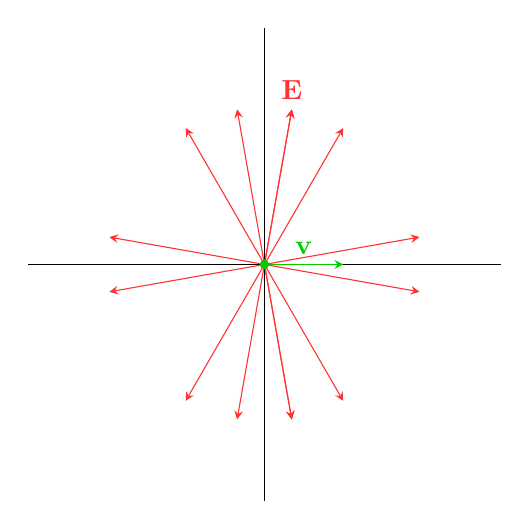
\begin{tikzpicture}
			\draw (-3, 0) -- (3, 0);
			\draw (0, -3) -- (0, 3);
			\draw[green!80!black, -stealth] (0, 0) -- (1, 0) node[midway, above] {\( \mathbf{v} \)};

			% horizontal lines
			\draw[-stealth, red!80!white] (0, 0) -- (10:2);
			\draw[-stealth, red!80!white] (0, 0) -- (-10:2);
			\draw[-stealth, red!80!white] (0, 0) -- (-170:2);
			\draw[-stealth, red!80!white] (0, 0) -- (170:2);
			
			% vertical lines
			\draw[-stealth, red!80!white] (0, 0) -- (80:2) node[above] {\( \mathbf{E} \)};
			\draw[-stealth, red!80!white] (0, 0) -- (-80:2);
			\draw[-stealth, red!80!white] (0, 0) -- (280:2);
			\draw[-stealth, red!80!white] (0, 0) -- (-280:2);
			\draw[-stealth, red!80!white] (0, 0) -- (260:2);
			\draw[-stealth, red!80!white] (0, 0) -- (-260:2);
			\draw[-stealth, red!80!white] (0, 0) -- (60:2);
			\draw[-stealth, red!80!white] (0, 0) -- (120:2);
			\draw[-stealth, red!80!white] (0, 0) -- (-60:2);
			\draw[-stealth, red!80!white] (0, 0) -- (-120:2);

			\filldraw[green!80!black] (0, 0) circle (0.05);
		\end{tikzpicture}
	\end{center}
	As for the \( \mathbf{B} \) field, we know that \( \mathbf{B} = \frac{1}{c}\hat{\brcurs} \times
	\mathbf{E} \), so:
	\[
		\mathbf{B} = \frac{1}{c} \frac{\brcurs}{\rcurs} \times \mathbf{E} = \frac{1}{c \rcurs} \left(
		\mathbf{R} + \frac{\rcurs}{c} \mathbf{v} \right) \times \left( \frac{q}{4\pi \epsilon_0}
	\frac{\mathbf{\hat{R}}}{R^2} \frac{1 - v^2 / c^2}{(1 - \frac{v^2}{c^2}\sin^2 \theta)^{3 / 2}} \right)
	\]
	Becuase \( \mathbf{\hat{R}} \times \mathbf{\hat{R}} = \mathbf{0} \), only the second term survives. This
	gives us a \( \mathbf{B} \) field that circles around the particle:
	\begin{center}
		\begin{tikzpicture}[decoration={markings,mark=at position 0.5 with {\arrow{stealth}}}]
			\draw[thick,-stealth] (-2,0) -- (2.5,0) node[right] {$x$};
			\draw[thick,stealth-stealth] (0,-1.5) -- (0,1.5) node[left] {$y$};
			\draw[very thick,green!70!blue!50,-stealth] (0,0) -- (0.75,0) node[below] {$\vec{v}$};
			\filldraw[green!70!blue!50] (0,0) circle (0.05cm);
			\draw[thick,orange!70!white,postaction={decorate}] (0,0) ellipse (-0.25cm and 1cm);
			\filldraw[white] (-0.3,0.125) rectangle (-0.2,-0.125);
			\draw[thick] (-0.31,0) -- (-0.19,0);
			\draw[thick,orange!70!white,postaction={decorate}] (-1.5,0) ellipse (-0.1cm and 0.4cm);
			\filldraw[white] (-1.65,0.125) rectangle (-1.55,-0.125);
			\draw[thick] (-1.66,0) -- (-1.54,0);
			\draw[thick,orange!70!white,postaction={decorate}] (1.5,0) ellipse (-0.1cm and 0.4cm);
			\filldraw[white] (1.35,0.125) rectangle (1.45,-0.125);
			\draw[thick] (1.34,0) -- (1.46,0);
		\end{tikzpicture}
	\end{center}
	We also talked about an intuitive way to think about this, called the \textbf{Thomson Kink Model}. To be
	completely honest, I can't explain this part of it better than Griffiths does, so just read examples 10.4
	and 10.5 there for a better description. 
\end{example}

	\section{April 7}
Today, we will begin discussing chapter 11, which is about radiation. Specifically, this chapter will deal
with fields which decay as \( \frac{1}{r} \), as opposed to \( \frac{1}{r^2} \) as we typically see in
electrostatics. We have to handle these fields with care, because quantities like the power:
\[
	P = \oint_{r \to \infty} \frac{1}{\mu_0} (\mathbf{E} \times \mathbf{B}) \diff \mathbf{a} = \text{finite}
\]
are finite for such fields even as \( r \to \infty \). In this sense, we sometimes say that the energy is
able to "detach" away from the sources and propagate all the way to infinity. From Jefimenko's equations, 
\begin{align*}
	\mathbf{E} &= \frac{1}{4\pi \epsilon_0} \int \left[ \frac{\rho(t_r, \mathbf{r}')}{\rcurs^2} \hat{\brcurs}
	+ \frac{\dot \rho (t_r, \mathbf{r}')}{c \rcurs} \hat{\brcurs} - \frac{\dot{\mathbf{J}} (t_r,
\mathbf{r}')}{c^2 \rcurs} \hat{\brcurs}\right] \diff \tau' \\ 
\mathbf{B} &= \frac{\mu_0}{4\pi} \int \left[ \frac{\mathbf{J}(t_r, \mathbf{r}')}{\rcurs^2} \times
\hat{\brcurs} + \frac{\mathbf{J}(t_r, \mathbf{r}')}{c\rcurs} \times \hat{\brcurs}\right] 
\end{align*}
Based on these equations, the terms with \( \frac{1}{r} \) dependence are the \( \dot \rho \) and \(
\dot{\mathbf{J}} \) terms. In order to calculate the radiation field, we will make some approximations:
\begin{enumerate}[label=\arabic*.]
	\item \( r \gg d \), where \( d \) is the length scale for the size of the source.   
	\item \( \lambda \simeq \frac{c}{\omega} \gg d \). This is used to suppress the details concerning the
		structure of the source itself. 
	\item \( T \ll \frac{r}{c} \) or \( \frac{1}{\omega} \ll \frac{r}{c} \). This assumption ensures that the
		time varying changes in the source have a significant impact.  
\end{enumerate}

\begin{example}[Electric Dipole Radiation]
	To illustrate a sample calculation, we will use the situation of electric dipole radiation. Consider a
	positive and negative charge separated by a distance \( d \), oscillating according to \( q(t) = q_0 \cos
	(\omega t)\).   
	\begin{center}
		\begin{tikzpicture}[decoration = {markings, mark=at position 0.5 with {\arrow{>}}}]
			\filldraw[red] (0, 1) circle (0.02) node[left] {\( +q \)};
			\filldraw[blue] (0, -1) circle (0.02) node[left] {\( -q \)};
			\draw[postaction=decorate] (0, 1) -- (0, -1) node[midway, left] {\( \mathbf{I} \)};
		\end{tikzpicture}
	\end{center}
	Given this, the current is \( I = qv = -q_0 \omega \sin(\omega t) \mathbf{\hat{z}} \). We can also
	calculate the potential very easily, as it is given by:
	\[
		V(\mathbf{r}, t) = \frac{1}{4\pi \epsilon_0} \frac{q_0 \cos\left[ \omega \left( t -
		\frac{\rcurs_+}{c} \right) \right]}{\rcurs_+(t_r)} - \frac{1}{4\pi \epsilon_0} \frac{q_0 \cos\left[
		\omega\left( t - \frac{\rcurs_-}{c} \right) \right]}{\rcurs_- (t_r)}
	\]
	Now, we can calculate the approximations we need separately. First, we will need to approximate \(
	\rcurs_{\pm} \):
	\[
		\rcurs_{\pm} = \sqrt{r^2 + \left(\frac{d}{2}\right)^2 \mp r d \cos \theta} \approx r \left( 1 \mp
		\frac{d}{2r}\cos \theta \right) \implies \frac{1}{\rcurs_{\pm}} \approx \frac{1}{r}\left( 1 \pm
	\frac{d}{2r} \cos \theta \right)
	\]
	here, we used the approximation that \( (1 + x)^{n} \approx 1 + nx \) when \( x \ll 1 \), suppressing the higher order
	terms. This uses the first assumption of \( \frac{d}{r} \ll 1 \). Next, we have the approximation of the
	argument in the cosine:
	\[
		\omega \left( t - \frac{\rcurs_{\pm}}{c} \right) = \frac{\omega}{c} \left[ ct - r\left( 1 \mp
		\frac{d}{2r} \cos \theta \right) \right] \approx \omega t - \frac{\omega r}{c} \pm \frac{d}{2(c /
	\omega)} \cos \theta + \dots
	\]
	Therefore, we can now evaluate the cosine using the addition rule:
	\begin{multline*}
		\cos\left[ \omega\left(t - \frac{\rcurs_{\pm}}{c}\right) \right] = \cos\left( \omega t - \frac{\omega
		\rcurs_{\pm}}{c} \right) \approx \cos\left[ \omega\left( t - \frac{r}{c} \right) \pm \frac{\omega
d}{2c} \cos \theta \right] 
\\ = \cos\left[ \omega\left( t - \frac{r}{c} \right) \right] \cos\left[ \frac{\omega d}{2c} \cos \theta
\right] \mp \sin \left[ \omega\left( t - \frac{r}{c} \right) \right] \sin\left[ \frac{\omega d}{2c}\cos \theta \right]
	\end{multline*}
	So now going back to \( V(\mathbf{r}, t) \):
	\begin{multline*}
			V(\mathbf{r}, t) = 
			\frac{q_0}{4\pi \epsilon_0}\frac{1}{r} \bigg\{ \left( 1 + \frac{d}{2r}\cos
			\theta \right) \left[ \cos \left( \omega\left( t - \frac{r}{c} \right) \right) - \sin\left[
		\omega\left( t - \frac{r}{c} \right) \right] \frac{wd}{2c}\cos \theta \right]  \\ 
							 - \left( 1 - \frac{d}{2r}\cos \theta \right) \left[ \cos \left[ \omega \left( t - \frac{r}{c} \right)
\right] + \sin \left[ \omega\left( t - \frac{r}{c} \right) \right] \frac{\omega d}{2c} \cos \theta
\right]\bigg\}
	\end{multline*}
	Now using the small angle approximation (\( \sin \theta \approx \theta \), \( \cos \theta \approx 1 \)), this simplifies to:
	\[
		V(\mathbf{r}, t) \simeq \frac{q_0d}{4 \pi \epsilon_0} \frac{1}{r^2} \cos \theta \cos\left[
		\omega\left( t - \frac{r}{c} \right) \right] - \frac{1}{4\pi \epsilon_0} \frac{q_0d \cos \theta}{r}
		\left( \frac{\omega}{c} \right) \sin\left[ \omega \left( t - \frac{r}{c} \right) \right]
	\]
	The first term is the dipole potential from electrostatics, and the second term is the radiation term,
	indicated by its \( \frac{1}{r} \) dependence. A similar approach can be taken to calculate \( \mathbf{A} \):
	\[
		\mathbf{A} = \frac{\mu_0}{4\pi} \int \frac{\mathbf{J}(t_r, \mathbf{r})}{\rcurs} \diff \tau' =
		-\frac{\mu_0}{4\pi} \int_{- d /2}^{d / 2} \frac{q_0 \omega \sin \left[ \omega \left( t - \frac{\rcurs}{c} \right)
		\right] \mathbf{\hat{z}}}{\left[ r^2 - 2 z' r \cos \theta + (z')^2 \right]^{1 / 2}} \diff z'
	\]
	Note that we integrate over \( z' \) here becuase \( \mathbf{J} \) generated by \( \mathbf{I} \) is only
	in the \( \mathbf{\hat{z}} \) direction. As for the bounds of the integral, this is given by the motion
	of the two charges. So, the integral becomes:
	\begin{align*}
		\mathbf{A} &= -\frac{\mu_0 q_0 \omega \mathbf{\hat{z}}}{4\pi} \int_{- d / 2}^{d / 2} \frac{1}{r}\left( 1 +
		\frac{z'}{2r}\cos \theta \right) \sin \left[ \omega\left( t - \frac{r}{c} \right) + \frac{\omega
	z'}{2c} \cos \theta  \right] \diff z'\\
	&= - \frac{\mu_0 q_0 \omega}{4\pi} \mathbf{\hat{z}} \int_{- d / 2}^{d /2} \frac{1}{r} \left( 1 + \frac{z'}{2r}\cos \theta
	\right) \left\{ \sin \left[ \omega\left(t - \frac{r}{c}\right) \right] \cos\left( \frac{\omega z'}{2c} \cos
	\theta\right) + \cos \left[ \omega\left( t - \frac{r}{c} \right) \right] \sin\left( \frac{\omega
z'}{2c}\cos \theta \right) \right\}  \diff z'
	\end{align*}
	Now, we will make some approximations. In particular, the function \( \frac{z'}{2r} \cos \theta \) is
	odd, so over an even interval it just goes to zero. Secondly, the \( (z')^2 \) terms are on the order of
	\( d^3 \), which is considered small compared to the length scale of the integral, so we ignore these
	terms as well. Therefore, the overall integral just simplifies to:
	\[
		\mathbf{A} \approx - \frac{\mu_0 q_0 \omega}{4\pi} \frac{d}{r} \sin \left[ \omega\left( t -
		\frac{r}{c} \right) \right] \mathbf{\hat{z}}
	\]
\end{example}	


	\section{April 9}
Last lecture, we found \( V \) and \( \mathbf{A} \), and with these fields determined we can get the \(
\mathbf{E} \) and \( \mathbf{B} \) fields:
\begin{align*}
	\mathbf{E} &= \frac{\mu_0 p_0 \omega^2}{4\pi} \left( \frac{\sin \theta}{r} \right)\cos\left[ \omega\left(
		t - \frac{r}{c}\right) \right] \boldsymbol{\hat{\theta}}\\
	\mathbf{B} &= - \frac{\mu_0 p_0 \omega^2}{4\pi c} \left( \frac{\sin \theta}{r} \right) \cos \left[
		\omega\left( t - \frac{r}{c} \right) \right] \boldsymbol{\hat{\phi}}
\end{align*}
here, we denote \( p_0 = qd \) is the polarization and \( q = q_0 \cos (\omega t) \) is an oscillating
charge. There are a couple things to note about this equation. Firstly, the \( \mathbf{E} \) and \(
\mathbf{B} \) oscillate in perpendicular directions, which makes sense given what we learned in chapter 9.
Further, these results are also consistent with our conclusion that the \( \mathbf{E} \) and \( \mathbf{B} \)
fields are in phase with each other, which is also what we found in chapter 9. With the \( \mathbf{E} \) and
\( \mathbf{B} \) fields, we can now figure out the Poynting vector:
\[
	\mathbf{S} = \frac{1}{\mu_0}(\mathbf{E} \times \mathbf{B}) = \frac{\mu_0}{c}\left\{ \frac{p_0
	\omega^2}{4\pi}\left( \frac{\sin \theta}{r} \right)\cos\left[ \omega\left( t - \frac{r}{c} \right)
\right] \right\}^2 \mathbf{\hat{r}}
\]
As a time-averaged quantity:
\[
	\mean{\mathbf{S}} = \frac{\mu_0 p_0^2 \omega^2}{32 \pi^2 c} \frac{\sin^2 \theta}{r^2}\mathbf{\hat{r}}
\]
What's interesting to note about this is that the time averaged \( \mathbf{S} \) is pointing in the \(
\mathbf{\hat{r}} \) direction, which is exactly perpendicular to the oscillation direction. This is what we
found in chapter 9, albeit through an intuitive argument back then. Here, we see the explicit mathematical
derivation.  

\subsection{Rayleigh and Mie Scattering}
When considering the interaction between light and particles, there are two limits that we can consider. The
first of which is when the wavelength of light is much larger than the size of the particle. In this limit,
because the particles are so small, we can essentially view them as vibrating coherently with the incoming
electric field, and therefore they radiate dipole radiation coherently. 

In this situation, the primary contribution of the waves comes from the dipole radiation, and therefore the
radiated electromagnetic wave is frequency dependent (you can see this via the \( \omega^2 \) dependence
above). This dependence explains why the sky is blue -- when the light from the sun scatters off molecules 
in the atmosphere (\( \mathrm{O_2, N_2, H_2} \)), the light scatters off them via dipole radiation. Further,
since the power scales proportional to \( \omega^{4} \), this heavily favors large frequencies, which is why
we see the sky as primarily blue. This phenomenon is known as \textbf{Rayleigh Scattering}. 

The other limit is when we consider the size of the particle to be much larger than the wavelength. In this
limit, the wave nature of the EM waves is suppressed, and in this case the light bounces off these materials
just like particles off a mirror. In this case, there is no frequency dependence, and this phenomenon
explains why clouds are white -- water molecules are on the order of 1mm, whereas light waves have
wavelengths on the order of 500nm, so all the light bounces off equally, leaving us with white clouds. This
phenomenon is called \textbf{Mie Scattering}.  

\subsection{Magnetic Dipoles}
Now, we will consider discussing magnetic dipoles. Consider the following situation, where we have a loop
with a current \( I = I_0 \cos(\omega t) \) shown in the diagram:

\begin{center}
	\begin{tikzpicture}[scale=1.5]
		\draw[thick,-stealth] (0,0) -- (0,2) node[right] {$z$};
		\draw[thick,-stealth] (0,0) -- (2,0) node[right] {$y$};
		\draw[thick,-stealth,rotate=-45] (0,0) -- (0,-2) node[below] {$x$};
		\draw[densely dashed] (0,1.75) -- (-0.9,0.85) -- (-0.9,-0.9);
		\draw[thick,-{Stealth[length=3pt]},blue!70!cyan!60] (-0.9,0.85) -- (-0.5,0.85) node[below,scale=0.5] {$\hat{\phi}=\hat{y}$};
		\filldraw[black] (-0.9,0.85) circle (0.025cm) node[left,scale=0.75] {$P$};
		\draw[thick,orange!70!white] (0,0) ellipse (0.99cm and 0.33cm);
		\draw[thick,-stealth,orange!70!white] (0,0) -- (1,0) node[midway,above,scale=0.5] {$b$};
		\draw[densely dotted] (0,0) -- (0.32,-0.32);
		\draw[-{Stealth[length=2pt]}] (0.32,-0.32) -- (0.55,-0.28) node[midway,below,scale=0.4] {$d\mathbf{l}'$};
		\draw[rotate=-45] (0.15,0) arc (0:-90:0.15cm) node[midway,below,scale=0.35] {$\phi$};
		\node[scale=0.75] at (1,1) (a) {$I = I_0\cos(\omega t)$};
		\draw[-{Stealth[length=2pt]},red!40!white] (-0.98,-0.08) node[left,scale=0.35] {$d\vec{e}'$} -- (-0.85,-0.27);
\end{tikzpicture}
\end{center}

We want to find the electric and magnetic fields over all space.
As always, the vector potential can be calculated using:
\[
	\mathbf{A} = \frac{\mu_0}{4\pi}\int \frac{\mathbf{J}(\mathbf{r}, t - \rcurs / c)}{\rcurs} \diff \tau' =
	\frac{\mu_0}{4\pi} \int \frac{I(\mathbf{r}, t - \rcurs / c)}{\rcurs} \diff \mathbf{l}'
\]
The reason we can write it in this form is because of the following relation for current density:
\( J \diff \tau = J A \diff l = I \diff l \). Now although \( \diff \mathbf{l} \) has both an \( x \) and \(
y\)-component, the \( x \) component will eventually cancel due to the symmetry in the system. Thus, we're
only left with the \( y \)-component. Because we need only care about the \( y \) component, then we may
write:
\[
	\mathbf{A} = \frac{\mu_0}{4\pi} \mathbf{\hat{y}} \int \frac{I(\mathbf{r}, t - \rcurs / c)}{\rcurs} \cos
	\phi' \diff \mathbf{l}'
\]
We will now use the approximations we had from earlier: \( b \ll r \), \( \frac{c}{\omega} \sim \lambda \gg b
\) and \( r \gg \frac{c}{\omega} \). Making these approximations, we eventually get the formula:
\[
	\mathbf{A}(\mathbf{r}, t) \simeq -\frac{\mu_0 m_0}{3\pi}\frac{\omega}{c}\left( \frac{\sin \theta}{r}
	\right) \sin\left[ \omega\left( t - \frac{r}{c} \right) \right]\boldsymbol{\hat{\phi}}
\]
You can verify this by explicitly computing the integral; in the interest of time we won't compute it here.
Since \( \rho = 0 \), then \( V = 0 \), so the \( \mathbf{B} \) field comes directly out of \( \nabla \times
\mathbf{A}\):
\[
	\mathbf{B} = \nabla \times \mathbf{A} = -\frac{\mu_0 m_0 \omega^2}{4 \pi c^2}\left( \frac{\sin \theta}{r}
	\right)\cos\left[ \omega\left( t - \frac{r}{c} \right) \right]\boldsymbol{\hat{\theta}}
\]
The \( \mathbf{E} \) field can be found using \( -\partial_t \mathbf{A} \):
\[
	\mathbf{E} = -\partial_t \mathbf{A} = \frac{\mu_0 m \omega^2}{4\pi c}\left(\frac{\sin \theta}{r}
	\right)\cos\left[ \omega\left( t - \frac{r}{c} \right) \right]\boldsymbol{\hat{\phi}}
\]
With \( \mathbf{B} \) and \( \mathbf{E} \), we may now calculate the power:
\[
	P_m = \int \mean{\mathbf{S}} r^2 \sin \theta \diff \theta \diff \Omega = \frac{\mu_0 m_0^2 \omega^{4}}{12
	\pi c^{3}}
\]
Now, with the electric dipole calculated from last lecture, we can now compare the power radiated by both the
electric and magnetic dipole:
\[
	\frac{P_m}{P_e} = \frac{1}{c^2}\left(\frac{m_0^2}{P_0^2}\right) = \frac{1}{c^2}\left( \frac{\pi I_0
	b^2}{qd} \right)^2 \sim \frac{\omega^2 b^2}{c^2}
\]
To get the approximation, we use \( I_0 = q \omega \) and use \( b \sim d \), because we assume the electric
and magnetic sources are on the same scale. Now, because we've assumed earlier that \( b \ll \frac{c}{\omega}
\), this implies \( \omega b / c \ll 1 \), hence \( P_m \ll P_e \). This shows that the electric power
dominates the magnetic power under our assumption, and this explains why we only focused on \( \mathbf{E} \)
waves in chapter 9.




	\section{April 11}
\subsection{Radiation for an Arbitrary Source Distribution}
Now that we've looked at radiation for specific source configurations, we will now look at how to calculate
the radiation emitted by an arbitrary source distribution. Consider an arbitrary ball of sources, for which
we want to find the field \( V(\mathbf{r}, t) \) everywhere. Well, the equations don't change, so:
\[
	V(\mathbf{r}, t) = \frac{1}{4\pi \epsilon_0} \int \frac{\rho(\mathbf{r}, t_r)}{\rcurs} \diff \tau'
\]
Calculating this for a general source is usually hard, so we will make some simplifying approximations.
First, because the radiation field dominates at large \( r \), we will make the approximation that \( r \gg
r' \), so that the \( \frac{1}{r^2} \) terms have already died out. With this assumption, we can approximate
\( \rcurs \):
\[
	\rcurs = \sqrt{r^2 + r'^2 + 2 \mathbf{r} \cdot \mathbf{r}'} \simeq r \left( 1 - \frac{\mathbf{r} \cdot
	\mathbf{r}'}{r^2} \right)
\]
Using the approximation that \( (1 + x)^{n} \approx 1 + nx \) when \( x \) is small (and indeed, \(
\mathbf{r}\cdot \mathbf{r}' / r^2 \) is small since the denominator is quadratic in \( r \)), then we can
write \( 1 / \rcurs \):
\[
	\frac{1}{\rcurs} = \frac{1}{r}\left( 1 + \frac{\mathbf{r} \cdot \mathbf{r}'}{r^2} \right)
\]
So, we can now Taylor expand \( \rho \):
\[
	\rho(\mathbf{r}, t - \rcurs / c) = \rho\left( \mathbf{r}', t - \frac{r}{c} + \frac{\mathbf{r} \cdot
	\mathbf{r}'}{c} \right) \approx \rho(\mathbf{r}, t_0) + \dot \rho(\mathbf{r}, t_0) \left(
	\frac{\mathbf{\hat{r}} \cdot \mathbf{r}'}{c} \right) + \frac{1}{2} \ddot \rho (\mathbf{r}', t_0) \left(
	\frac{\mathbf{\hat{r}} \cdot \mathbf{r}'}{c} \right)^2
\]
Now, we impose our second assumption, this one being on \( \dot \rho \) and the higher derivative terms. We
will assume that the time variation must be fast enough. This is enforced through the ratios:
\[
	\left| \frac{\ddot \rho}{\dot \rho} \right|, \left| \frac{\dddot \rho}{\ddot \rho} \right|, \left|
	\frac{\rho^{4}}{\dddot \rho} \right|, \dots \ll \frac{c}{r'}
\]
You can essentially think of this as requiring that the wavelength of the waves is much larger than the
structure size, or mathematically \( \mathbf{r}' \ll cT \simeq \lambda \). Intuitively this also makes sense,
since high frequency waves die out and don't make it very far, and what's left are the low frequency waves
with large \( \lambda \). Practically speaking, what this approximation does is allow us to keep only the
first order \( \mathbf{r}' \) terms. Therefore, our \( V(\mathbf{r}, t) \) becomes:
\begin{align*}
	V(\mathbf{r}, t) &= \frac{1}{4\pi \epsilon_0} \frac{1}{r}\left[ \int \rho(\mathbf{r}, t_0) \diff \tau' +
	\frac{\mathbf{\hat{r}}}{r} \int \mathbf{r}' \rho(\mathbf{r}', t_0) \diff \tau' +
\frac{\mathbf{\hat{r}}}{c} \dv{t} \int \mathbf{r}' \rho(\mathbf{r}', t_0) \diff \tau' \right]\\
&= \frac{1}{4\pi \epsilon_0}\frac{Q}{r} + \frac{1}{4\pi \epsilon_0} \frac{\hat{\mathbf{r}} \cdot \mathbf{p}(t_0)}{r^2} 
+ \frac{1}{4\pi \epsilon_0} \frac{\hat{\mathbf{r}} \dot{\mathbf{p}}(t_0)}{cr}	
\end{align*}
For the second term, we use the fact that the electric dipole moment is defined as
\( \mathbf{p} = \int \mathbf{r}' \rho(\mathbf{r}') \diff \tau \) to simplify it. The first two terms should
be familiar: these are the multipole expansion terms, and the third one is due to radiation. The third term
ends up being the only term we care about, since when we calculate the gradient of the potential the third
term is the only one that produces a \( \frac{1}{r} \) dependence term. 
 
For the vector potential, we have the equation:
\[
	\mathbf{A} = \frac{\mu_0}{4\pi} \int \frac{\mathbf{J}(\mathbf{r}, t_r)}{\rcurs} \diff \tau
\]
Since \( J = \rho v \), computing an integral like \( \int \mathbf{J} \diff \tau \) is essentially the same
as summing over each individual charge:
\[
	\int \mathbf{J} \diff \tau \sim \sum_i q_i v_i = \sum_i q_i \dv{\mathbf{r}'_i}{t} = \dv{t} \sum_i q_i
	\mathbf{r}'_i \sim \dot{\mathbf{p}}(t_0)
\]
so we can loosely approximate such an integral as the time derivative of the dipole moment. Then, because \(
\int \mathbf{J} \diff \tau \) is already on the order of \( \mathbf{r}' \), any other higher order terms will
be second order corrections, and hence we can just take \( \frac{1}{\rcurs} \simeq \frac{1}{r} \). All in
all, the relevant potentials are:
\[
	V \simeq \frac{1}{4\pi \epsilon_0} \frac{\mathbf{r} \cdot \mathbf{p}(t_0)}{cr} \quad \mathbf{A} \simeq
	\frac{\mu_0}{4\pi} \frac{\dot{\mathbf{p}}(t_0)}{r}
\]
To find the field, we now take \( \mathbf{E} = -\nabla V - \partial_t A \) and \( \mathbf{B} = \nabla
\times \mathbf{A} \) as usual. Starting with \( \nabla V \), recall that the only term we care about in \( V
\) is the third term, so:
\[
	(\nabla V)_i = \frac{1}{4\pi \epsilon_0} \frac{1}{cr} \nabla \left[ \mathbf{\hat{r}} \cdot
	\dot{\mathbf{p}}(t_0) \right]
\]
Now the gradient:
\[
	\partial_i p^{j}(t_0) = (\partial_i t_0) \ddot p^{j}(t_0) = -\frac{1}{c} \hat{r}_i \ddot p^{j}(t_0)
\]
where we use \( \partial_j t_0 = -\frac{1}{c} \nabla r \). Now, written in vector form:
\[
	(\nabla V)_i = -\frac{1}{4\pi \epsilon_0} \frac{\mathbf{\hat{r}} \cdot \ddot{\mathbf{p}}(t_0)}{rc^2}
	\mathbf{\hat{r}} 
\]
The \( \partial_t \mathbf{A} \) term is easy:
\[
	\partial_t \mathbf{A} = \frac{\mu_0}{4\pi} \frac{\ddot{\mathbf{p}}(t_0)}{r}
\]
So putting these two together to get \( \mathbf{E} \):
\[
	\mathbf{E} = -\frac{1}{4\pi \epsilon_0} \frac{\mathbf{\hat{r}} \cdot
	\ddot{\mathbf{p}}(t_0)}{rc^2}\mathbf{\hat{r}} - \frac{\mu_0}{4\pi} \frac{\ddot{\mathbf{p}}(t_0)}{r} =
	\frac{\mu_0}{4\pi} \left[ \mathbf{\hat{r}} \times (\mathbf{\hat{r}} \times \ddot{\mathbf{p}}(t_0) \right]
\]
where we've used the vector triple product identity \( \mathbf{a} \times (\mathbf{b} \times \mathbf{c}) =
\mathbf{b}(\mathbf{a} \cdot \mathbf{c}) - \mathbf{c}(\mathbf{a} \cdot \mathbf{b}) \) to write it in its final
form. To find \( \mathbf{B} \), we use \( \mathbf{B} = \nabla \times \mathbf{A} \):
\[
	\mathbf{B} = \nabla \times \mathbf{A} = \frac{\mu_0}{4\pi} \epsilon^{ijk}\partial_j \dot p_k(t_0) =
	\frac{\mu_0}{4\pi} \epsilon^{ijk} (\partial_j t_0) \ddot p_k
\]
Again using \( \partial_j t_0 = -\frac{1}{c} \nabla r \), we have:
\[
	\mathbf{B} = \frac{\mu_0}{4\pi r} \epsilon^{ijk} \left( -\frac{1}{c} \hat{r}_j \right) \ddot p_k =
	-\frac{\mu_0}{4\pi cr} \left[ \mathbf{\hat{r}} \times \ddot{\mathbf{p}}(t_0) \right]
\]
Notice that indeed we have \( \mathbf{B} = \frac{1}{c}\mathbf{\hat{r}} \times \mathbf{E} \), you can check
this for yourself also if you'd like. 

\begin{example}
	Under the special case \( \mathbf{p} = p \mathbf{\hat{z}} \), \( \dot{\mathbf{p}} = \dot{p}
	\mathbf{\hat{z}} \), and \( \ddot{\mathbf{p}} = \ddot{p} \mathbf{\hat{z}} \) (i.e. one-dimensional motion),
	then the \( \mathbf{E} \) and \( \mathbf{B} \) fields take the form:
	\begin{align*}
		\mathbf{E} &= \frac{\mu_0 \ddot p(t_0)}{4\pi}\left( \frac{\sin \theta}{r} \right)
		\boldsymbol{\hat{\theta}} \\ 
		\mathbf{B} &= \frac{\mu_0 \ddot p(t_0)}{4\pi c}\left( \frac{\sin \theta}{r} \right)\boldsymbol{\hat{\phi}} 
	\end{align*}
	Combined, we can calculate \( \mathbf{S} \):
	\[
		\mathbf{S} = \frac{1}{\mu_0}(\mathbf{E} \times \mathbf{B}) = \frac{\mu_0 [\ddot{p}(t_0)]^2}{16 \pi^2
		c}\left( \frac{\sin \theta}{r} \right)^2 \mathbf{\hat{r}}
	\]
	So the power is:
	\[
		P = \int \mathbf{S} \cdot \diff \mathbf{a} = \frac{\mu_0 [\ddot{p}(t_0)]^2}{16 \pi^2 c} \int \frac{\sin^2
		\theta}{r^2} (r^2 \sin \theta) \diff \theta \diff \phi = \frac{\mu_0 [\ddot p(t_0)]^2}{6 \pi c}
	\]
	In the case of a point charge, we have \( \mathbf{p} = q \mathbf{d} \), and hence \( \ddot{\mathbf{p}} =
	q \ddot{\mathbf{a}} = qa \mathbf{\hat{z}} \), so the power becomes:
	\begin{equation}
		\label{Larmor}
		P = \frac{\mu_0 q^2 a^2}{6 \pi c}
	\end{equation}
	This is the well-known \textbf{Larmor Formula}, which gives the power radiated by a point charge. Notice
	that it only radiates power when it is accelerated. We will revisit this formula and derive it from a
	different perspective next week.
\end{example}

 
 
 

	\section{April 14}
\subsection{Radiation of a Moving Point Charge}
Recall that at the end of last lecture, we derived the Larmor formula (\cref{Larmor}), which relates the
radiation of a point charge to its acceleration. While the previous derivation does indeed work, it's not
exactly very satisfying (at least in my view), since you still make the approximation that a point charge is
a charge enclosed in a very small volume. We will correct this by deriving the Larmor formula through a
completely different means, which doesn't involve such an assumption.  

To begin this analysis, we start off with a diagram:
\begin{center}
	\begin{tikzpicture}[>=Stealth, scale=3.5]

	  \draw[dotted] (0, 0) circle (0.5);

	  % Red dot representing \vec{r}(t)
	  \filldraw[red] (0,0) circle (0.02);
	  \node[below left=-0.1, red] at (0.07,-0.07) {$\vec{w}(t)$};

	  % Blue vector from center to boundary
	  \coordinate (C) at (0,0);
	  \coordinate (T) at (30:0.5);
	  \draw[->, thick, blue] (C) -- (T) node[above right] {\( t_s \)};

	  \draw[dashed] (160:1) .. controls (-0.5, 0.3) and (-0.2, 0.1) .. (0, 0) 
							.. controls (0.2, -0.1) and (0.5, -0.3) .. (345:1);

	\end{tikzpicture}
\end{center}
We regard the particle as having position given by \( \mathbf{w}(t) \), and its signal emitted at time \( t
\) reaches our sphere at time \( t_s \). In this context, \( t \) is considered the retarded time. Now,
recall that for a moving particle, we derived earlier that the electric field follows:
\[
	\mathbf{E}(r, t_s) = \frac{q}{4\pi \epsilon_0} \frac{\rcurs}{(\brcurs \cdot \mathbf{u})^2} \left[ (c^2 -
	v^2) \mathbf{u} + \brcurs \times (\mathbf{u} \times \mathbf{a}) \right]
\]
Recall that the first term represents the velocity field, and the second represents the acceleration field.
The \( \mathbf{B} \) field follows \( \mathbf{B} = \frac{1}{c}\mathbf{\hat{r}} \times \mathbf{E} \) as usual.
Our goal is to derive the Larmor formula, so we want to find an expression for the power \( P(t) \) coming
out of the particle, which is the same power that arrives to the sphere at time \( t_s \). As usual, the
power is a surface integral of the Poynting vector \( \mathbf{S} \), so:
\[
	\mathbf{S} = \frac{1}{\mu_0}(\mathbf{E} \times \mathbf{B}) = \frac{1}{\mu_0c}(\mathbf{E} \times
	\hat{\brcurs} \times \mathbf{E}) = \frac{1}{\mu_0c}\left[ |\mathbf{E}|^2 \hat{\brcurs} -
	\mathbf{E}(\mathbf{E} \cdot \hat{\brcurs}) \right]
\]
Because we are only considering the radiation field, we can drop the velocity field since it doesn't go as \(
\frac{1}{\rcurs}\). Given this assumption, this means that \( \mathbf{E} \) is approximately proportional to
\( \brcurs \times (\mathbf{u} \times \mathbf{a}) \), and hence the second term which has an \( \mathbf{E}
\cdot \brcurs \) term will die. Therefore, the final equation for \( \mathbf{S} \) is:
\[
	\mathbf{S} = \frac{1}{\mu_0c}|\mathbf{E}|^2 \hat{\brcurs}
\]
Now we look to simplify the \( \mathbf{E} \) term from this equation. To do this, we will first assume tat \(
v = 0\) but \( a \neq 0 \); this may look like a strange assumption at first, but bear with me as we derive
this and eventually generalize to the \( v \neq 0 \) case. Under these assumptions, then \( \mathbf{u} = c
\hat{\brcurs} - \mathbf{v} = c \hat{\brcurs}\):
\begin{align*}
	\mathbf{E} &= \frac{q^2}{16 \pi^2 \epsilon_0^2} \frac{\rcurs^2}{ (\rcurs^3 c^3)^2} \left| c^3
	\hat{\brcurs} + c \brcurs \times (\hat{\brcurs} \times \mathbf{a}) \right|^2\\
			   &= \frac{q^2}{16 \pi^2 \epsilon_0^2} \frac{1}{\rcurs^{4} c^{6}}\left| c^3 \hat{\brcurs} + c
			   \hat{\brcurs} (\mathbf{a} \cdot \brcurs) - \mathbf{a} \brcurs \right|^2 
\end{align*}
From here, we only take terms that are proportional to \( \rcurs^2 \) -- this is so that we get only the \(
\sim \frac{1}{\rcurs^2} \) terms for \( \mathbf{S} \), and from there when integrating we get out only the \(
\frac{1}{\rcurs}\) terms. Now, expanding the square:
\begin{align*}
	|\mathbf{E}|^2 &= \frac{q^2}{16 \pi^2 \epsilon_0^2} \frac{1}{r^{4}c^{6}} \left( c^2 a^2 \rcurs^2 +
	c^2(\mathbf{a} \cdot \brcurs)^2 - 2c^2 (\mathbf{a} \cdot \brcurs)^2 \right)\\
	&= \frac{\mu_0^2 q^2}{16 \pi^2} \frac{1}{\rcurs^{4}} \left( a^2 \rcurs^2 - (\mathbf{a} \cdot \brcurs)^2 \right) 
\end{align*}
Now, \( \mathbf{a} \cdot \rcurs \) is the same as \( a \rcurs \cos \theta \) by definition of the dot
product, so this now simplifies to:
\[
	|\mathbf{E}|^2 = \frac{\mu_0^2 q^2}{16 \pi^2} \frac{a^2}{\rcurs^2} \sin^2 \theta
\]
So now we have our final expression for \( \mathbf{S} \):
\[
	\mathbf{S} = \frac{\mu_0 q^2 a^2}{16 \pi^2 c}\left( \frac{\sin^2 \theta}{\rcurs^2} \right) \hat{\brcurs}
\]
Finally, the power:
\[
	P = \oint \mathbf{S} \diff \mathbf{a} = \frac{\mu_0 q^2 a^2}{16 \pi^2 c} \int_{0}^{\pi} \sin^2 \theta
	\sin \theta \diff \theta \int_{0}^{2\pi} \diff \phi = \frac{\mu_0 q^2 a^2}{6 \pi c}
\]
which is exactly the Larmor formula, this time derived without the assumption of volume. It should also be
clear after this derivation that the Larmor formula only works when \( v = 0 \), as that was one of the
assumptions we made to simplify \( \mathbf{E} \). Generally, this is a pretty good approximation anyways for
\( v \ll c \), but to be completely formal, when \( v \neq 0 \) we have to consider not only the fact that \(
\mathbf{E}\) changes but \( \mathbf{S} \) changes too. To see this, consider a moving particle, and think
about the number of wavefronts emitted over a given time interval, versus the number of wavefronts received
at a distance away:
\begin{center}
	\begin{tikzpicture}
		\filldraw[red] (0,0) circle (0.1) node[below=0.2] {particle};
		\draw[dashed] (60:1) arc [start angle = 60, end angle = -60, radius = 1];
		\draw[dashed] (60:1.5) arc [start angle = 60, end angle = -60, radius = 1.5];
		\draw[dashed] (60:1.9) arc [start angle = 60, end angle = -60, radius = 1.9];
		\draw (4, 1) -- (4, -1) node[below] {screen};
	\end{tikzpicture}
\end{center}
Because of this velocity, you can check that the effective wavelength \( \lambda_\text{eff} = (c - v) T \),
where \( T \) is the period between the wavefronts. 
The number of wavefronts received \( N_\text{receive} \) is given by:
\[
	N_\text{receive} = \frac{(c \Delta t) / \lambda_\text{eff}}{\Delta t} = \frac{c}{(c - v)T} = \left(
	\frac{c}{c - v} \right)N_\text{emit}
\]
Now in the general case only the velocity in the direction of emission matters, so we replace \( v \) with \(
\mathbf{v} \cdot \brcurs \), giving us the formula:
\[
	N_\text{emit} = \left( 1 - \frac{\mathbf{v} \cdot \brcurs}{c} \right)N_\text{receive}
\]
We will continue this discussion next time and see how this subtlety affects the power emitted.  
 
 
 
  

	\section{April 16}
\subsection{Lienard Formulation}
Last lecture, we left off with our discussion of a general formula for the power radiated by a particle when
\( v \neq 0 \). Picking up where we left off, we concluded last that the power emitted and the power received
at a time \( t_s \) later may be written as:
\begin{align*}
	\dv{W}{t} &= \dv{W}{t_s} \left( 1 - \frac{\brcurs \cdot \mathbf{v}}{c} \right)\\
			  &= \dv{W}{t_s}\left( 1 - \left( c \rcurs - \brcurs \cdot \mathbf{v} \right) \right) \\ 
			  &= \dv{W}{t_s} \frac{1}{c\rcurs} (\mathbf{u} \cdot \rcurs) 
\end{align*}
Now our \( \mathbf{E} \) field is of the form:
\[
	\mathbf{E} = \frac{q}{4\pi \epsilon_0} \frac{\rcurs}{(\brcurs \cdot \mathbf{u})}\left[ \brcurs \times (c
	\mathbf{\hat{r}} \times \mathbf{a})\right]
\]
Now, the power emitted by the particle may be written as \( P = \int \mathbf{S} \diff \mathbf{a} \), and the
infinitesimal area may be decomposed as \( \diff \mathbf{a} = r^2 \diff \Omega \), where \( \Omega \)
represents the solid angle. Thus, we may write \( \dv{P}{\Omega} \) as:
\[
	\dv{P}{\Omega} = \underbrace{\frac{1}{\mu_0c} \left( \frac{q^2}{16 \pi^2 \epsilon_0^2}
			\frac{\rcurs^2}{(\brcurs \cdot \mathbf{u})^{6}}\left|\brcurs \times (\mathbf{u} \times \mathbf{a})\right|^2 
	\right)}_{\mathbf{S}} \cdot \rcurs^2
\]
Ordinarily this would be fine, but to account for the velocity of the particle, we have to scale this by the
factor introduced at the beginning of the lecture:
\[
	\dv{P}{\Omega} = \frac{1}{\mu_0c} \left( \frac{q^2}{16 \pi^2 \epsilon_0^2} \frac{\rcurs^2}{(\brcurs \cdot
	\mathbf{u})^{6}}\left|\brcurs \times (\mathbf{u} \times \mathbf{a})\right|^2 \right) \cdot \rcurs^2
	\left( \frac{\mathbf{u} \cdot \brcurs}{c\rcurs} \right) = \frac{q^2}{16 \pi^2 \epsilon_0} \frac{|\brcurs
	\times (\mathbf{u} \times \mathbf{a})|^2}{(\hat{\brcurs} \times \mathbf{u})^{5}}
\]
The power then, is this this integral over the solid angle:
\begin{equation}
	\label{lienard}
	P = \oint \dv{P}{\Omega} \sin \theta \diff \theta \diff \phi = \frac{\mu_0 q^2 \gamma^{6}}{6 \pi c}\left(
	a^2 - \left| \frac{\mathbf{v} \times \mathbf{a}}{c} \right|^2 \right)
\end{equation}
This is called the \textbf{Lienard generalization} of the Larmor formula. Notice the factor of \( \gamma \)
present in the numerator, meaning that the added contribution due to the velocity (from the first term) is
very negligible, until we get to speeds \( v \sim c \).   


\subsection{Bremsstrahlung (Braking Radiation)}
This occurs particularly in the case where \( \mathbf{v} \parallel \mathbf{a} \). So, first we calculate some
cross products:
\[
	\mathbf{u} \times \mathbf{a} = (c \hat{\brcurs} - \mathbf{v}) \times \mathbf{a} = c
	\mathbf{\hat{\brcurs}} \times \mathbf{a} \implies \hat{\brcurs} \times (\mathbf{u} \times \mathbf{a}) = c
	\hat{\brcurs} \times (\hat{\brcurs} \times \mathbf{a}) = c \hat{\brcurs} (\hat{\brcurs} \cdot \mathbf{a})
	- c \mathbf{a}
\]
Thus, the numerator \( |\brcurs \times (\mathbf{u} \times \mathbf{a})|^2 \) becomes:
\[
	 |\brcurs \times (\mathbf{u} \times \mathbf{a})|^2 = c^2(a^2 + (\mathbf{a} \cdot \hat{\brcurs})^2 -
	 2(\mathbf{a} \cdot \hat{\brcurs}^2) = a^2 c^2 (1 - \cos^2 \theta) = c^2 a^2 \sin^2 \theta
\]
The denominator \( \hat{\brcurs} \cdot \mathbf{u} \) becomes:
\[
	\hat{\brcurs} \cdot \mathbf{u} = \hat{\brcurs} \cdot (c \hat{\brcurs} - \mathbf{v}) = c - \mathbf{v}
	\cdot \hat{\brcurs} = c - v \cos \theta = c(1 - \beta \cos \theta)
\]
we define \( \beta = v / c \). Therefore, putting this all together:
\[
	\dv{P}{\Omega} = \frac{q^2}{16 \pi^2 \epsilon_0^2} \frac{\left| \hat{\brcurs} \times(\mathbf{u} \times
	\mathbf{a}) \right|^2}{(\hat{\brcurs} \cdot \mathbf{u})^{5}} = \frac{\mu_0 q^2 a^2}{16 \pi^2 c}
	\frac{\sin^2 \theta}{(1 - \beta \cos \theta)^{5}}
\]
There is also a maximum angle that the radiation is shot out of, which you will do for homework. 
\begin{example}[Stability of "Classical" Hydrogen Atom]
	Consider the classical model of a Hydrogen atom, with a proton with \( +e \) charge in the center and an
	electron orbiting it at a distance of \( R \sim 10^{-10} \) m. Classically, the energy of the particle is
	given by:
	\[
		U = \frac{1}{2}mv^2 - \frac{ke^2}{R}
	\]
	According to the formula for centripetal force:
	\[
		\frac{ke^2}{R} = m a_c = \frac{mv^2}{R} \implies \frac{1}{2} mv^2 = \frac{ke^2}{2R}
	\]
	combining this with the previous equation yields a total energy of:
	\[
		E = - \frac{ke^2}{2R}
	\]
	This numerically comes out to about -13.6 eV, the well known ground state energy of hydrogen. From this
	calculation, we can also deduce \( v \), which comes out to roughly \( v \sim 10^{-2}c \), so this motion
	is still considered non-relativistic. So, we can use the Larmor formula:
	\[
		P = \frac{\mu_0 q^2 a^2}{6 \pi c}
	\]
	Now that we know accelerating particles give off radiation, so given that the electron radiates energy
	how long does it take before it loses enough energy to crash onto the proton? Well, we can calculate that
	now:
	\[
		\dv{E}{t} = -P = -\frac{\mu_0 q^2 a^2}{6 \pi c} \quad \dv{t} \left( - \frac{ke^2}{2r} \right) =
		\frac{\mu_0 q^2}{6 \pi c} \left( \frac{v^2}{r} \right)^2 = - \frac{\mu_0 q^2}{6 \pi c}\left(
		\frac{ke^2}{mr^2} \right)^2
	\]
	equating the two, we now have a differential equation in \( r \):
	\[
		\frac{ke^2}{2r^2} \dv{r}{t} = - \frac{\mu_0 q^2}{6 \pi c} \left( \frac{ke^2}{mr^2} \right)^2
	\]
	doing separation of variables and integrating to the characteristic time \( \tau \), we get:
	\[
		\tau = \frac{4\pi^2 \epsilon_0^2}{e^{4}} m^2 c^3 R_0^3 \sim 10^{-11} \text{ seconds}
	\]
	This is \textit{really bad!} Obviously this is not true, and it's one of the many things that motivated
	quantum mechanics. As you know, quantum mechanics doesn't treat the electron as a physical object around
	the atom but rather models its position as a wavefunction, resolving this paradox.   
\end{example}








	\section{April 18}
\subsection{Self-Force/Radiation Reaction}
Recall the Larmor formula for nonrealtivistic particles:
\[
	P_\text{rad} = \frac{\mu_0 q_0^2 a^2}{6 \pi c}
\]
From this formula, it may be natural to assume that the power, which is also written as \( \mathbf{F} \cdot
\mathbf{v} = - P_\text{rad} \), but this is \textit{not} true! The reason for this is because the Larmor
formula only considers radiation that extends to infinity, so the power contributed by the velocity field is
missing. 

However, because energy continuously flows in and out of the velocity field, it is possible for us to still
use the above formula, just only when the net velocity of the particle is zero. For periodic motion, this
would mean that we can consider the motion over a time interval \( \tau \) where the particle returns to the
same place, at which point the contribution by the velocity field should be zero. Thus:
\begin{align*}
	\int_{0}^{T} \mathbf{F} \cdot \mathbf{v} \diff t &= - \int_{0}^{T} \frac{\mu_0 q^2 a^2}{6 \pi c} \diff
	t\\
	 &= - \int_{0}^{T} \frac{\mu_0 q^2}{6 \pi c}
	 \dv{\mathbf{v}}{t} \dv{\mathbf{v}}{t} \diff t \\ 
	 &= \int_{0}^{T} \frac{\mu_0 q^2}{6 \pi c} \dv[2]{\mathbf{v}}{t} \cdot \mathbf{v} \diff t - 
	 \int_{0}^{T} \dv{t} \left( \frac{\mu_0 q^2}{6 \pi c} \dv{\mathbf{v}}{t} \mathbf{v} \right) \diff t	
\end{align*}
The second term equals zero if the particle returns to the same spot. This leaves us with the equality:
\[
	\int_{0}^{T} \mathbf{F} \cdot \mathbf{v} \diff t = \int_{0}^{T} \frac{\mu_0 q^2}{6 \pi c}
	\dv[2]{\mathbf{v}}{t} \mathbf{v} \diff t
\]
comparing the integrands, we get the result:
\[
	\mathbf{F}_\text{rad} = \frac{\mu_0 q^2}{6 \pi c} \dv[2]{v}{t}
\]
This is known as the \textbf{Abraham-Lorentz} formula. However, this is not a very rigorous way to obtain this
equation. Firstly, not all motion is periodic, so why does this formula work for nonperiodic motion too?
Secondly, this only tells you about the self-force for the component \( \mathbf{F}_\text{rad} \) that is
along the direction of \( \mathbf{v} \), since the integrand is really \( \mathbf{F} \cdot \mathbf{v} \) on
the left hand side. So we need an alternative method to derive this formula.    

Before we do though, there is something interesting about this formula that we can point out right away. When
forces have \( \dot{\mathbf{a}} \) dependence, invoking Newton's second law:
\[
	\frac{\mu_0^2 q^2}{6 \pi c} \dot{\mathbf{a}} = m \mathbf{a}
\]
this is a differential equation for the acceleration, with solution \( a(t) = a_0 e^{t / \tau} \), and \(
\tau \) is the prefactor on \( \dot{\mathbf{a}} \). The interesting thing is that \( a(t) \) is now increasing
with increasing time, meaning the acceleration gets faster and faster as you go on. Conversely, if you insist
that \( a = 0 \), then you will find that if you do try to apply an external force, the particle starts
responding to that force before you even act on it. Obviously both of these solutions are non-physical, but so
far there is no mathematical reason why we should reject them. 

\subsection{The Dumbbell Model}
Now, we move on to finding a better way to derive the Abraham-Lorentz formula. To do so, we use a so-called
\textit{dumbbell model}, in which we split a charge into a tiny dumbbell with half the charge each:  
\begin{center}
	\begin{tikzpicture}
		\coordinate (positive1) at (1, 2.5);
		\coordinate (negative1) at (1, 0.8);

		\coordinate[-stealth] (positive2) at (3, 2.5);
		\coordinate[-stealth] (negative2) at (3, 0.8);

		\draw (-1, 0) -- (4, 0) node[right] {\( x \)};
		\draw (0, -1) -- (0, 3) node[left] {\( y \)};
		\filldraw[red] (positive1) circle (0.03) node[left] {\( +q / 2 \)};
		\filldraw[blue] (negative1) circle (0.03) node[left] {\( -q / 2 \)};

		\draw (positive1) -- node[midway, left] {\( d \)} (negative1);

		\filldraw[red] (positive2) circle (0.03) node[right] {\#1};
		\filldraw[blue] (negative2) circle (0.03) node[right] {\#2};

		\draw[dashed] (positive1) -- (positive2);
		\draw[dashed] (negative1) -- node[midway, below] {\( \ell \)} (negative2);
	\end{tikzpicture}
\end{center}
Recall that the equation for the field of moving charges is given by:
\[
	\mathbf{E}(\mathbf{r}, t) = \frac{q}{4\pi \epsilon_0} \frac{\rcurs}{\brcurs \cdot \mathbf{u}} \left[ (c^2
	- v^2) \mathbf{u} + \brcurs \times (\mathbf{u} \times \mathbf{a}) \right]
\]
For simplicity of the model, we will assume that \( v(t_r) = 0  \) so that \( \mathbf{u} = c \hat{\brcurs}
\), and \( \mathbf{a} = a \mathbf{\hat{x}} \). 
Now, let's consider the force on charge \#1 due to charge \#2. In this case, we have:
\[
	\brcurs = \ell \mathbf{\hat{x}} + d \mathbf{\hat{y}}, \quad \hat{\brcurs} = \frac{\ell \mathbf{\hat{x}} +
	d \mathbf{\hat{y}}}{\sqrt{\ell^2 + d^2}}
\]
This makes the triple cross product:
\[
	\brcurs \times (\mathbf{u} \times \mathbf{a}) = (\brcurs \cdot \mathbf{a}) \mathbf{u} - (\brcurs \cdot
	\mathbf{u}) \mathbf{a}
\]
Notice that we also only need to consider the \( x \)-component, since the \( y \)-components will cancel
each other when you add the forces on both charges (due to symmetry). Therefore, the force on 1 may be
written as:
\[
	\mathbf{E}_{1x} = \frac{q / 2}{4\pi \epsilon_0} \frac{\sqrt{\ell^2 + d^2}}{c \sqrt{\ell^2 + d^2}} \left[ c^3
	\frac{\ell}{\sqrt{\ell^2 + d^2}} + \ell a \frac{c\ell}{\sqrt{\ell^2 + d^2}} - ca\sqrt{\ell^2 + d^2} \right] =
	\frac{q}{8\pi \epsilon_0} \frac{1}{c^2(\ell^2 + d^2)^{3 /2}} \left( lc^2 - d^2 \right)\mathbf{\hat{x}}
\]
By symmetry \( E_{2x} \) is the exact same. Therefore, the self force may be written as:
\[
	\mathbf{F}_\text{self} = \left( \frac{q}{2} \right) \mathbf{E}_{1x} + \left( \frac{q}{2} \right)
	\mathbf{E}_{2x} = \frac{q^2}{8 \pi \epsilon_0 c^2} \frac{\ell c^2 - d^2}{(\ell^2 + d^2) ^{3 /
	2}}\mathbf{\hat{x}}
\]
so far this treatment is exact, but we ultimately want to model the situation in the \( d \to 0 \) limit
so we need to Taylor expand the above equation in orders of \( d \). We can't immediately Taylor expand this
just yet, since \( \ell \) also has \( d \) dependence that we need to expand. To begin, we note that \( \ell
= x(t) - x(t_r) \), so we first Taylor expand \( x(t) \) around \( t = t_r \):
\[
	x(t) = x(t_r) + \dot x(t_r) (t - t_r) + \frac{\ddot x(t_r)}{2}(t - t_r)^2
\]
Noting that \( t - t_r = T \) and \( \dot x(t_r) = 0 \) so the second term dies, we can write \( \ell \) as:
\begin{equation}
	\label{ell}
	\ell = \frac{1}{2} \ddot x(t_r) T^2 + \frac{1}{6} \dddot x(t_r) T^3 + \dots 
\end{equation}
simultaneously, we have a relation for \( \ell \) based on pure geometry:
\[
	d = \sqrt{(cT)^2 - \ell^2} = \sqrt{1 - \frac{1}{c^2 T^2} \left( \frac{1}{2} aT^2 + \frac{1}{6} \dot a T^3 +
	\dots \right)} \approx cT - \frac{a^2 T^3}{8c}
\]
reversing this equation and solving for \( T \):
\[
	T = \frac{d}{c} + \frac{a^2}{8c^2}\left( \frac{d}{c} \right)^3 + \dots
\]
Putting this back into \cref{ell} we finally have \( \ell \) in terms of \( d \):
\[
	\ell = \frac{1}{2}a \left( \frac{d}{c} \right)^2 + \frac{1}{6}\dot a \left( \frac{d}{c} \right)^3 +
	O(d^{4}) 
\]
Thus, we now have:
\[
	\mathbf{F}_\text{self} = \frac{q^2}{8 \pi \epsilon_0 c^2} \frac{\ell c^2 - ad^2}{(\ell^2 + d^2)^{3 / 2}}
	\simeq \frac{q^2}{8 \pi \epsilon_0 c^2} \left[ -\frac{a}{2d} + \frac{\dot a}{6c} + O(d^2) \right]
\]
Notice that we have a term proportional to \( a \). In some sense, this term can be regarded as an effective
mass term. To see what this means, consider Newton's second law with \( \mathbf{F}_\text{self} \):
\[
	\left( -\frac{q^2}{16 \pi \epsilon_0d}\frac{1}{c^2} \right) a + \frac{q^2 \dot a}{4 \pi \epsilon_0}
	\frac{1}{3c^2} = m_0a
\]
but we can rearrange this equation into:
\[
	\frac{q^2 \dot a}{4 \pi \epsilon_0} \frac{1}{3c^2} = \left( m_0 + \frac{q^2}{16 \pi \epsilon_0 d}
	\frac{1}{c^2} \right)a
\]
Notice how the factor of \( \frac{q^2}{16 \pi \epsilon_0 d} \) acts as "extra mass" in addition to \( m_0 \),
which is why it is sometimes called the effective mass term. Looking at this term in close detail, you can
see why we can regard it this way. This term denotes the potential energy between the two charges, and as a
form of energy based on Einstein's equation \( E = mc^2 \) we know that energy and mass are closely
connected. So, in light of this it does make sense that you can regard this energy as a form of extra mass. 

	\section{April 21}
\subsection{Self-Force}
Last lecture, we left off with the equation:
\begin{equation}
	\label{abraham-lorentz-partial}
	\frac{q^2 \dot a}{12 \pi \epsilon_0 c^2} = \left( m_0 + \frac{1}{4\pi \epsilon_0} \frac{(q / 2)^2}{d}
	\right)a
\end{equation}
where we now have an added term on the right as an "added mass" term due to the velocity of the particle.
Based on the way we've structured this equation, you can regard the left hand side as the \( \mathbf{F}_\text{rad} \)
that we're looking for. However, you may notice that this formula is off by a factor of \(1 / 2\),
and the reason for this is so far we've only considered the contribution from one \( q / 2 \) to the other \(
q / 2\) charge, but didn't consider the self force on the \( q / 2 \) charges \textit{themselves}.  

To reconcile this, suppose we have:
\[
	\mathbf{F}_\text{rad}(q) = \mathbf{F}_\text{rad, int}\left( \frac{q}{2} \right) 
	+ \mathbf{F}_\text{rad, self}\left( \frac{q}{2}\right)
\]
Now we break each of the \( q / 2 \) charges into dumbbells with charge \(  q / 4 \), so now:
\[
	\mathbf{F}_\text{rad} \left( \frac{q}{2} \right) = \mathbf{F}_\text{rad, int}\left( \frac{q}{4} \right) +
	2 \mathbf{F}_\text{rad, self}\left( \frac{q}{4} \right)
\]
Here, we can drop the "self" subscript in \( \mathbf{F}_\text{rad, self} \) since the force itself is a
self-force, so it's functionally the same as \( \mathbf{F}_\text{rad} \). Using this fact, we move it to the
left hand side. Then, if you keep iterating this process, making smaller and smaller dumbbells, you
eventually get the system:
\begin{align*}
	\mathbf{F}_\text{rad}(q) - 2 \mathbf{F}_\text{rad}\left( \frac{q}{2} \right) &= \mathbf{F}_\text{rad,
	int}\left( \frac{q}{2} \right)\\
		2 \mathbf{F}_\text{rad}\left( \frac{q}{2} \right) - (2\times 2) \mathbf{F}_\text{rad}\left( \frac{q}{4} \right) &= 2
	\mathbf{F}_\text{rad, int} \left( \frac{q}{4} \right)\\
	4 \mathbf{F}_\text{rad}\left( \frac{q}{4} \right) - (4 \times 2)\mathbf{F}_\text{rad}\left( \frac{q}{8}
	\right) &= \mathbf{F}_\text{rad, int}\left( \frac{q}{4} \right)\\
			&\vdots
\end{align*}
We now add all these equations up together, and we see that the left hand telescopes to \(
\mathbf{F}_\text{rad}(q) \). The right hand side, using our partial result (\cref{abraham-lorentz-partial}),
we get:
\[
	\mathbf{F}_\text{rad}(q) = \frac{\mu_0 \dot a q^2}{3 \pi c} \cdot \frac{1}{4} \left( 1 + \frac{1}{2} +
	\frac{1}{4} + \frac{1}{16} + \dots \right) = \frac{\mu_0 \dot a q^2}{12 \pi c} \frac{1}{1 - 1 / 2} =
	\frac{\mu_0 \dot a q^2}{6 \pi c}
\]
which is exactly the Abraham-Lorentz formula. This also concludes our discussion of chapter 11, and we now
move on to special relativity. 

A small foreword on the special relativity section: it does \textbf{not} follow chapter 12 of Griffiths, but
instead Chien-I's own provided notes. When I wrote up these notes, the content between the chapters is
relatively similar, but it should be noted that there will be differences at times (especially in the last
two lectures).    
  

\subsection{Special Relativity}
To begin the topic of special relativity, a good place to start are the fundamental postulates of special
relativity. These are:
\begin{enumerate}[label=\arabic*.]
	\item Physical laws should be the same in all \textbf{inertial} reference frames. 
	\item Motivated by Maxwell's equations \( c = \frac{1}{\sqrt{\mu_0 \epsilon_0}} \). Based on postulate 1,
		this implies that the speed of light is constant in all inertial reference frames. 
\end{enumerate}
Before we begin our discussion of special relativity is it interesting to note that while the second
postulate seems rather arbitrary, it is in fact quite a natural thing to suppose: the constants \( \mu_0 \)
and \( \epsilon_0 \) govern the strength of electric and magnetic fields, so if we are to believe the first
postulate, then we cannot believe \( \mu_0 \) or \( \epsilon_0 \) to change between reference frames -- and
from here the constancy of \( c \) across reference frames drops out. 

With these postulates established, simultaneity is now broken! Consider a situation where Alice is at rest
(\( v = 0 \)) and Bob is in a rocket ship moving at constant velocity \( v_0 \). As the rocket ship passes by
Alice, Bob emits two EM signals, which travel in opposite directions, as shown in the diagram below:
\begin{center}
	\begin{tikzpicture}[scale=1.5]
    \foreach \x/\y/\color/\opacity in {0/0/black/1,0/-1/black/0.5,1.5/-1/blue!70!cyan!40/0.6,3/-1/blue!40!cyan!60/0.7} {
        \draw[thick,color=\color,opacity=\opacity] (\x,\y) rectangle (\x+2.25,\y+0.5);
    }
    \foreach \pos in {(0.15,0.225), (0.15,-0.775)} {
        \node at \pos (a) {\Strichmaxerl[1.5]};
        }
    \foreach \x/\y/\color/\opacity in {0.4/0.1/black/1,0.4/0.4/black/1,0.4/-0.9/black/0.5,1.9/-0.6/blue!70!cyan!40/0.6,3.4/-0.9/blue!40!cyan!60/0.7} {
        \draw[thick,color=\color,opacity=\opacity] (\x,\y) -- (\x+0.25,\y);
    }
    \foreach \pos/\opacity in {(0,0.25)/1,(0,-0.75)/0.4} {
        \node[scale=0.5,thick,draw,isosceles triangle,minimum size=2pt,isosceles triangle apex angle=90,xshift=-0.3cm,opacity=\opacity] () at \pos {};
    }
    \draw[orange!70!white,-{Stealth[length=2pt]}] (0.425,0.15) -- (0.425,0.35);
    \draw[orange!70!white,-{Stealth[length=2pt]}] (0.625,0.35) -- (0.625,0.15);
    \draw[orange!70!white,-{Stealth[length=2pt]}] (0.525,-0.85) -- (2.015,-0.65) node[midway,above,scale=0.5] {$D'$};
    \draw[orange!70!white,-{Stealth[length=2pt]}] (2.035,-0.65) -- (3.525,-0.85) node[midway,above,scale=0.5] {$D'$};
    \foreach \x in {0.625,2.15} {
        \draw[green!70!blue!50] (\x,-1.1) -- (\x,-1.2);
    }
    \draw[green!70!blue!80] (0.625,-1.15) -- (2.15,-1.15) node[midway,below,scale=0.75] {$\frac12v\Delta t'$};
\end{tikzpicture}
\end{center}
From Bob's reference frame, because he is moving with the rocket, the two signals reach either end of the
ship simultaneously. However, in Alice's frame, the red signal reaches the left end before the right, because
the motion of the ship meant that the red signal had less distance to cover.
So, while Bob's reference frame preserves the simultaneity of both events, that simultaneity is broken
in Alice's reference frame, but Bob's frame is no more "correct" than Alice's. 

\subsection{Time Dilation}

Now suppose we have the following diagram, where Bob has a "clock" which sends a light signal up and down:
\begin{center}
	\begin{tikzpicture}[scale=1.5]
    \draw[thick] (0,0) rectangle (2.25,0.5);
    \node[scale=0.5,thick,draw,isosceles triangle,minimum size=2pt,isosceles triangle apex angle=90,xshift=-0.3cm] (a) at (0,0.25) {};
    \node at (1.125,0.225) (b) {\Strichmaxerl[1.5]};
    \node[scale=0.5] at (1.125,-0.1) (ll) {Bob};
    \node[scale=0.5] at (0,-0.2) (aa) {Alice};
    \node at (0,-0.5) (c) {\Strichmaxerl[1.5]};
    \draw[thick,-{Stealth[length=2pt]}] (1.125,0.6) -- (1.5,0.6) node[midway,above,scale=0.5] {$v$};
\end{tikzpicture}
\end{center}
If the distance between the two ends is \( D \), then the time measured by Bob would be \( \Delta t =
\frac{2D}{c} \). However, for Alice, due to the fact that the rocket ship is moving relative to her, would
see the time interval as:
\[
	\Delta t' = \frac{2D'}{c} = 2 \frac{\sqrt{\frac{1}{4} v^2 (\Delta t')^2 + D^2}}{c}
\]
Rearranging this to solve for \( \Delta t' \), we get:
\[
	\Delta t' = \frac{1}{\sqrt{1 - v^2 / c^2}}(\Delta t) = \gamma \Delta t
\]
This is the formula we are all familiar with to calculate time dilation. The factor \( \gamma \equiv
\frac{1}{\sqrt{1 - v^2 / c^2}} \) is a common one in relativity that you should be familiar with. We will
continue our discussion of this next time. 

	\section{April 23}
\subsection{Time Dilation/Proper time}
Last lecture, we covered the idea of time dilation, and derived the relation \( \Delta t = \gamma \Delta t'
\). In that example, we had Bob moving with the rocket ship, where the two events, the emission of the photon
and its absorption back occur at the same location in the \( S' \) frame. Because these two events occur at
the same location in the \( S' \) frame, the time difference measured in such a reference frame is called the
\textit{proper time}, and is denoted \( \Delta \tau \). This quantity will be important in our later
discussions. 

\subsection{Length Contraction}
Here, we touch on the topic of length contraction. Consider a situation below, where Bob is on a rocket ship
and Alice is standing by on a ledge as Bob goes past. Bob is holding a long rod, and at \( t = 0 \), the
front end of that rod passes by Alice. The length of the rod, as measured by Bob, is called the
\textit{proper length}, denoted by \( L_0 \). The proper length is the length measured by an observer that is
moving with no relative motion with the object in question (i.e. Bob). 

At some time \( \Delta t \) later, the back of the rod passes Alice, so for Alice she will measure the length
as \( L = v \Delta t \). Because Alice measures the rod at the same location, her length is denoted by the
proper time, \( L = v \Delta \tau \). For Bob, Alice moves over a distance \( L_0 \) in a time \( \Delta t'
\), with a speed \( v \). Therefore, Bob writes \( L_0 = v \Delta t' \). Because we know that \( \Delta t'
 = \gamma \Delta t\), then we get \( L_0 = v \gamma \Delta t = \gamma L \), and hence we get \( L =
 \frac{L_0}{\gamma} \), which is the standard formula for length contraction. Do note, however, that the
 lengths in the \textit{perpendicular} direction, are not contracted! You can see this by the fact that \(
 \gamma = 1 \) in that case.   

\subsection{Lorentz Boost/Transformation}
We now tackle the above phenomena from a theoretical perspective, by building up to Lorentz transformations.
Consider two frames \( \mathcal{S} \) and \( \mathcal{S}' \), where \( \mathcal{S}' \) travels with speed \(
v\). And, consider an event at time \( (t, x) \) in \( \mathcal{S} \). We now ask the question: what is the
relation between \( (t, x) \) and \( (t', x') \)?   

\begin{center}
	\begin{tikzpicture}
		\draw[-stealth] (0, 0) -- (3, 0);
		\draw[-stealth] (0, 0) -- (0, 3) node[above] {\( \mathcal{S} \)};
		\draw[-stealth, red] (1, 0) -- (4, 0);
		\draw[-stealth, red] (1, 0) -- (1, 3) node[above] {\( \mathcal{S}'\)} ;
		\draw[-stealth, red] (1.2, 2.5) -- (1.5, 2.5) node[right] { \( v \) };
		\filldraw[blue] (3.2, 0.5) circle (0.02) node[right] {\( (t, x) \)};
	\end{tikzpicture}
\end{center}
In Galilean relativity, the transformation would be:
\[
	t' = t \quad x' = x - vt
\]
because time is assumed to pass the same in different reference frames. However, as we shall see, this is not
the case in relativity. To see this more clearly, let's consider a specific situation: at \( t = 0 \), frame
\( \mathcal{S}' \) starts moving, and simultaneously a light pulse at \( (t, x) = (t', x') = (0, 0) \) is
sent out. At some time later, it travels a distance \( L_0 \) as measured in \( \mathcal{S}' \). 
 
\begin{center}
	\begin{tikzpicture}[decoration=snake]
		\draw[-stealth] (0, 0) -- (3, 0);
		\draw[-stealth] (0, 0) -- (0, 3) node[above left] {\( \mathcal{S} \)};
		\draw[-stealth, red] (0.1, 0) -- (3.1, 0);
		\draw[-stealth, red] (0.1, 0) -- (0.1, 3) node[above right] {\( \mathcal{S}'\)};
		\draw[-stealth, red] (0.3, 2.5) -- (0.7, 2.5) node[right] { \( v \) };
		\draw[red] (0.5, 0.5) rectangle node[midway, above=0.2] {\( L_0 \)} ++(3, 0.4);
		\draw[orange, -stealth, decorate] (0.5, 0.7) -- (1.2, 0.7);
		\node at (1.5, -0.5) {Event 1};
	\end{tikzpicture}
	\hspace{3cm}
	\begin{tikzpicture}[decoration=snake]
		\draw[-stealth] (0, 0) -- (3, 0);
		\draw[-stealth] (0, 0) -- (0, 3) node[above] {\( \mathcal{S} \)};
		\draw[-stealth, red] (1, 0) -- (4, 0);
		\draw[-stealth, red] (1, 0) -- (1, 3) node[above] {\( \mathcal{S}'\)} ;
		\draw[-stealth, red] (1.2, 2.5) -- (1.5, 2.5) node[right] { \( v \) };
		\draw[red] (1.4, 0.5) rectangle node[midway, above=0.2] {\( L_0 \)} ++(3, 0.4);
		\draw[orange, -stealth, decorate] (3.7, 0.7) -- (4.4, 0.7);
		\node at (1.5, -0.5) {Event 2};
	\end{tikzpicture}
\end{center}
In the \( \mathcal{S} \) frame, event 2 happens at a coordinate \( (\Delta t, \Delta x) \). Note that this is
both improper time and length, since the events are not occurring in the same location, and \( \mathcal{S} \)
is not moving with the length \( L_0 \). In the \( \mathcal{S}' \) frame though, event 2 happens at the
coordinates \( (\Delta t', L_0) \). Note the proper time here because \( \mathcal{S}' \) moves with the
length \( L_0 \). Given the formula for length contraction though, we can go ahead and calculate what \(
\Delta x \) should be:
\[
	\Delta x = v \Delta t + L = v \Delta t + \frac{L_0}{\gamma} = v \Delta t + \frac{\Delta x'}{\gamma}
	\implies \Delta x' = \gamma(\Delta x - v \Delta t)
\]
And we arrive at the familiar formula for a Lorentz boost in the \( x \)-direction.
For the time portion, we have \( \Delta t' = \frac{L_0}{c} \) for Bob, and for Alice we have:
\[
	\Delta t = \frac{\Delta x}{c} = \frac{1}{c}\left( v \Delta t + \frac{L_0}{\gamma} \right) =
	\frac{v}{c}\Delta t + \frac{\Delta t'}{\gamma} \implies \Delta t' = \left( 1 - \frac{v}{c} \right)
	\Delta t \cdot \gamma
\]
Hence, we have:
\[
	\Delta t = \frac{\Delta x'}{c} = \frac{\gamma}{c}\left( \Delta x - v \Delta t \right) = \gamma\left(
	\frac{\Delta x}{c} - \frac{v}{c}\Delta t \right) = \gamma\left( \Delta t - \frac{v}{c}\frac{\Delta x}{c} \right) 
	= \gamma\left(\Delta t - \frac{v}{c^2}\Delta x\right)
\]
Here, we arrive at the formula for the Lorentz boost for time. Both of these formulas can be summarized into
one transformation, called the \textit{Lorentz Boost} or Lorentz Transformation:
\[
	\begin{cases}
		\Delta t' = \gamma\left( \Delta t - \frac{v}{c^2}\Delta x \right)\\
		\Delta x' = \gamma(\Delta x - v \Delta t)\\
		\Delta y' = \Delta y \\
		\Delta z' = \Delta z
	\end{cases},
	\quad \gamma = \frac{1}{\sqrt{1 - v^2 / c^2}}
\]
Note that this is only in the \( x \)-direction, but the other directions are the exact same derivation. One
interesting thing about this transformation is that the following holds true:   
\[
	-(c \Delta t')^2 + (\Delta x')^2 = -(c \Delta t)^2 + (\Delta x)^2
\]
This equality really tells us something about what the Lorentz transformation does to our coordinate system.
Just like how under rotation, the Euclidean distance: \( (\Delta x')^2 + (\Delta y')^2 + (\Delta z')^2 \)
remains invariant, the above quantity is invariant under Lorentz transformation. In this sense, we can think
of \( (c \Delta t)^2 + (\Delta x)^2 \) as a notion of "length", which remains invariant under the Lorentz
transformation.
 
There also happens to be another way to write this equality, which is to use matrix notation:
\[
	\begin{pmatrix} c \Delta t & \Delta x & \Delta y & \Delta z \end{pmatrix} 
	\begin{pmatrix} -1 & & &\\ & 1 & & \\ & & 1 & \\ & & & 1\end{pmatrix}
	\begin{pmatrix} c \Delta t\\ \Delta x \\ \Delta y\\ \Delta z \end{pmatrix} = \text{const.}
\]
which can also be written more compactly as \( \eta_{\mu \nu}(\Delta x)^{\mu} (\Delta x)^{\nu} =
\text{const.} \). Our requirement that this remains invariant can then be written as:
\[
	\eta_{\mu \nu}(\Delta x)^{\mu}(\Delta x)^{\nu} = \eta_{\rho \sigma}(\Delta x)^{\rho}(\Delta x)^{\sigma}
\]
Notice that \( \Delta x \) is the same on both sides, but the \textit{metric} \( \eta_{\rho \sigma} \) does
not use the same indices. So how does this equation reflect invariance? As we'll see in the next lecture,
we've encoded the transformation in changing \( \eta_{\mu \nu} \to \eta_{\rho \sigma} \). 



	\section{April 25}
Recall that last time, we discussed the quantity \( -(c \Delta t)^2 + (\Delta x)^2 \) and its invariance.
More generally, we can adapt this invariance to include all three dimensions:
\[
	(\Delta s)^2 = -(c \Delta t)^2 + (\Delta x)^2 + (\Delta y)^2 + (\Delta z)^2 = \eta_{\mu \nu}(\Delta
	x)^{\mu}(\Delta x)^{\nu}
\]
and this quantity is usually called the \textit{spacetime interval}. As discussed last time as well, we
require that this quantity be invariant under Lorentz boosts and also spatial rotation. Here, we develop the
formal notation to discuss Lorentz transformations. We've already established that it is a transformation of
some kind, so it's natural to think about a point \( (\Delta x') \) as being derived by multiplying \( (\Delta
x) \) by some matrix \( \Lambda \):
\[
	(\Delta x')^{\mu} = \Lambda^{\mu}_{\nu}(\Delta x)^{\nu}
\]
Then, this notation implies that in the new frame, the spacetime interval is written as:
\[
	\begin{pmatrix} c \Delta t' & \Delta x' & \Delta y' & \Delta z' \end{pmatrix}
	\begin{pmatrix} -1 & & & \\ & 1 & & \\ & & 1 & \\ & & & 1 \end{pmatrix}
	\begin{pmatrix} c \Delta t'\\ \Delta x' \\ \Delta y' \\ \Delta z' \end{pmatrix} = (\Delta x')^{\top}
	\eta (\Delta x') = 
	(\Delta x)^{\sigma}(\Lambda^{\top})^{\rho}_{\sigma} \eta_{\rho \nu} \Lambda^{\mu}_\nu (\Delta x)^{\nu}
\]
\begin{aside}
	Notice that \( (\Delta x')^{\top} \) should be written as a dual vector, but we still write it using an
	upper index \( (\Delta x')^{\top} = (\Delta x)^{\sigma} (\Lambda^{\top})^{\rho}_\sigma \). The reason for
	this is because we want to treat the vector and dual vector on "equal footing", and treat the metric as
	the object such that when we combine the vector and dual together we get a scalar. We will explore this
	more in depth at a later lecture, so keep this in the back of your mind for now.    
\end{aside}

The statement of invariance means we want this to equal \( (\Delta x)^{\sigma} \eta_{\sigma \nu}(\Delta x)^{\nu} \),
so we have the equality:
\[
	(\Delta x)^{\sigma}(\Lambda^{\top})^{\rho}_\sigma \eta_{\rho \mu} \Lambda^{\mu}_{\nu}(\Delta x)^{\nu} =
	(\Delta x)^{\sigma}\eta_{\sigma \nu} (\Delta x)^{\nu}
\]
If we want these two quantities to be the same, then we should require that the Lorentz transformation does
not change the metric. We can see this as \( \Lambda^{\top} \eta \Lambda \) is the "new" metric on the left,
which we require it equal to the one on the right. So, this means we should have the equality: 
\[
	\Lambda^{\top} \eta \Lambda = \eta 
\]
or in index notation,
\[
	(\Lambda^{\top})^{\rho}_{\sigma} \eta_{\rho \nu} \Lambda^{\mu}_\nu = \eta_{\sigma \nu}
\]
Because \( (\Lambda^{\top})^{\rho}_\sigma = \Lambda^{\rho}_\sigma \) (by virtue of transpose) 
then this equation becomes:
\[
	\eta_{\rho \mu}\Lambda^{\rho}_\sigma \Lambda^{\mu}_\nu = \eta_{\sigma \nu}
\]
With this conclusion, we can say that the Lorentz transformation \( \Lambda^{\mu}_\nu \) is one that both
preserves the metric above, and also preserves the handedness (i.e. we want transformations that preserve \(
x \to x \) and not \( x \to -x \)). In terms of the actual form for \( \Lambda \), there are six of them:
\begin{align*}
	\Lambda &= \begin{pmatrix} \cosh \phi & -\sinh \phi & 0 & 0\\ -\sinh \phi & \cosh \phi & 0 & 0\\ 0 &0 & 1
	& 0\\ 0 & 0 & 0 & 1\end{pmatrix}, \quad \begin{pmatrix} \cosh \phi & 0 & -\sinh \phi & 0\\ 0 & 1 & 0 & 0
		\\ -\sinh \phi & 0 & \cosh \phi & 0\\ 0 & 0 & 0 & 1\end{pmatrix}, \quad \begin{pmatrix} \cosh \phi &
	0 & 0 & -\sinh \phi\\ 0 & 1 &0 & 0 \\ 0 & 0 & 1 & 0\\ -\sinh \phi & 0 & 0 & \cosh \phi\end{pmatrix}\\
	\\
		\Lambda &= \begin{pmatrix} \cos \theta & \sin \theta & 0 & 0 \\ -\sin \theta & \cos \theta & 0 & 0 \\
			0  &0 & 1 & 0\\ 0 & 0 & 0 & 1 \end{pmatrix}, \quad \begin{pmatrix} \cos \theta & 0 & \sin \theta
			   & 0 \\ 0 & 1 & 0 & 0 \\ -\sin \theta & 0 & \cos \theta & 0 \\ 0 & 0 & 0 & 1\end{pmatrix}, \quad
			\begin{pmatrix} \cos \theta & 0 & 0 & \sin \theta \\ 0 & 1 &0 & 0\\ 0 & 0 & 1 & 0\\ -\sin \theta
			& 0 & 0 & \cos \theta\end{pmatrix}
\end{align*}
The top row are Lorentz boosts in the \( x, y, z \) directions respectively, and the bottom row are rotations
about the \( z \) axis, \( x \) axis and \( y \) axes, respectively. As for the Lorentz boosts, it's easy to
check that \( (\Delta s')^2 = (\Delta s)^2 \) easily. Firstly, let's write out what the transformed vector
looks like:
\begin{equation}
	\label{lorentz-boost}
	\begin{pmatrix} c \Delta t' \\ \Delta x' \\ \Delta y' \\ \Delta z' \end{pmatrix} = \begin{pmatrix}  \cosh
\phi & -\sinh \phi & & \\ -\sinh \phi & \cosh \phi & & &\\ & & 1 & \\ & & & 1 \end{pmatrix} \begin{pmatrix} c
\Delta t \\ \Delta x \\ \Delta y \\ \Delta z \end{pmatrix}
\end{equation}
So \( (\Delta s')^2 \) is written as:
\begin{align*}
	\begin{split}
	-(c \Delta t')^2 + (\Delta x')^2 &= 
		-\cosh^2 \phi (c \Delta t)^2 - \sinh^2 \phi (\Delta x)^2 + 2 \cosh
		\phi (c \Delta t) \sinh \phi (\Delta x) + \sinh^2 \phi (c \Delta t)^2 \\ &+ \cosh^2 \phi - 2 \cosh \phi \sinh
		\phi (c \Delta t) (\Delta x)
		\end{split}
		\\
		&= [\cosh^2 \phi - \sinh^2 \phi](c \Delta t)^2 + [\cosh^2 \phi - \sinh^2 \phi] (\Delta x)^2
\end{align*}
Then using the identity that \( \cosh^2 \phi - \sinh^2 \phi = 1 \), then \( (\Delta s')^2 = (\Delta s)^2 \),
as required. There is also a physical meaning to this parameter \( \phi \) that we've seemingly mysteriously
introduced, which we can see from the physical interpretation of a Lorentz boost:
\[
	\begin{pmatrix} c \Delta t'\\ \Delta x' \\ \Delta y \\ \Delta z' \end{pmatrix}
	= 
	\begin{pmatrix} \gamma \left( c \Delta t - \frac{v}{c}\Delta x \right)\\ 
	\gamma \left( -\frac{v}{c^2} (c \Delta t) + \Delta x \right)\\
\Delta y \\ 
\Delta z\end{pmatrix}
\]
so comparing this with \cref{lorentz-boost}, we see that:
\[
	\cosh \phi = \gamma \quad \sinh \phi = \frac{\gamma v}{c}
\]
this implies \( \tanh \phi = \frac{\gamma v / c}{\gamma} = v / c \), so \( \phi = \tanh^{-1}(v / c) \). 

\subsection{4-Vectors}
So far in our discussion, the only 4-vector that we've encountered is this quantity \( (\Delta x)^{\mu} \)
that we've been talking about. More generally however, a 4-vector is defined as any vector that transforms in
the same way as \( (\Delta x)^{\mu} \) under a Lorentz transformation. That is:
\[
	V^{\mu} \to V'^{\mu} = \Lambda^{\mu}_\nu V^{\nu}
\]	
Not all \( V \) are valid 4-vectors! Take the following non-example: define \( \tilde u^{\mu} \) as follows:
\[
	\tilde u^{\mu} \equiv \dv{x^{\mu}}{t} = \begin{pmatrix} c \\ u \end{pmatrix}
\]
where \( u^{i} = \dv{x^{i}}{t} \). Then, under a Lorentz boost in the \( x \)-direction, we have:
\[
	\tilde u'^{\mu} = \begin{pmatrix} \dv{(ct')}{t}\\ \dv{x'}{t'} \\ \dv{y'}{t'} \\
	\dv{z'}{t'} \end{pmatrix} = \begin{pmatrix} c \\ \frac{\gamma(dx - v \diff t)}{\gamma
	(\diff t - \frac{v}{c^2} \diff x)}\\ \frac{dy}{\gamma(dt - \frac{v}{c^2} \diff x)} \\
	\frac{dz}{\gamma(dt - \frac{v}{c^2} \diff x)} \end{pmatrix} = 
	\begin{pmatrix} c \\ 
	\\
	\dfrac{u_x - v}{1 - \dfrac{v u_x}{c^2}} \\ 
	\\
	\dfrac{u_y}{\gamma\left( 1 - \dfrac{v u_x}{c^2} \right)}\\ 
	\\
	\dfrac{u_z}{\gamma\left( 1 - \dfrac{v u_x}{c^2} \right)}\end{pmatrix}
\]
The \( x \)-component transforms as:
\[
	u_x \to \frac{u_x - v}{1 - \frac{v u_x}{c^2}}
\]
is the familiar formula for velocity addition in lower division classes. Notice that a transformation like
this is non-linear (this should be obvious), and hence it doesn't transform like \( (\Delta x)^{\mu} \) so it
is not a valid 4-vector. 

As with all vectors, we can define an "inner product" with these vectors, which we define as \( \eta_{\mu
\nu} V^{\mu} W^{\nu} \). This inner product is particularly convenient because it's Lorentz invariant:
\[
	\eta_{\mu \nu}V'^{\mu}W'^{\nu} = \eta_{\mu \nu}\left( \Lambda^{\mu}_\rho V^{\rho} \right)\left(
	\Lambda^{\nu}_\sigma W^{\sigma} \right) = \eta_{\mu \nu} \Lambda^{\mu}_\rho \Lambda^{\nu}_\sigma V^{\rho}
	W^{\sigma} = \eta_{\rho \sigma} V^{\rho}W^{\sigma}
\]
The invariance is nice because it means that regardless of how you Lorentz boost, this is a quantity you can
calculate which is the same in all reference frames. For a particular 4-vector, we define it as space-like,
time-like, or light-like based on its inner product with itself:
\[
	V^2 = \eta_{\mu \nu}V^{\mu}V^{\nu} = \begin{cases}
		< 0 & \text{time-like}\\
		= 0 & \text{light-like} \\ 
		> 0 & \text{space-like}
	\end{cases}
\]
Finally, one last thing which we will take up next lecture: for \( V^{\mu} = (\Delta x)^{\mu} \), we are
constrained by the spacetime interval: \( -(c \Delta t)^2 + (\Delta x)^2 = \text{const.} \), this traces out
the shape of a \textit{hyperbola}! So when we perform a Lorentz transformation, what we essentially do is
move the vector \( (\Delta x)^{\mu} \) along its defined hyperbola, like in the diagram below: 

\begin{center}
	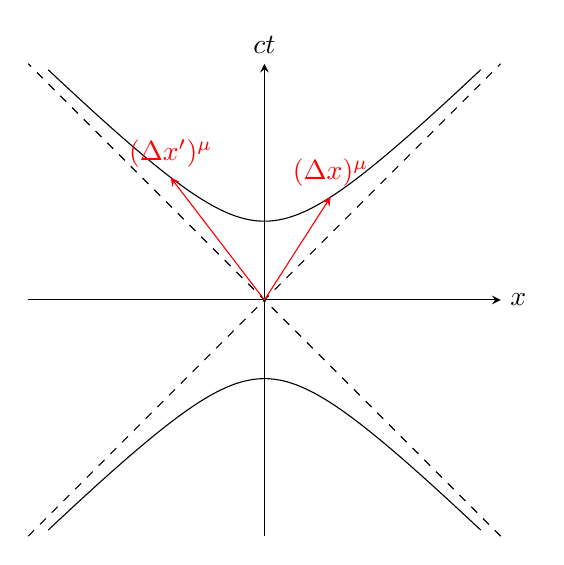
\begin{tikzpicture}
		\draw[-stealth] (-3, 0) -- (3, 0) node[right] {\( x \)};
		\draw[-stealth] (0, -3) -- (0, 3) node[above] {\( ct \)};
		\draw[dashed] (-3, -3 ) -- (3, 3);
		\draw[dashed] (3, -3) -- (-3, 3);
		\draw[rotate around={90:(0, 0)}] plot [variable = \t, samples=1000, domain=-70:70] 
			({1 / cos( \t )}, {1 * tan( \t )});
		\draw[rotate around={90:(0, 0)}] plot [variable = \t, samples=1000, domain=-70:70] 
			({-1 / cos( \t )}, {1 * tan( \t )});
		\draw[-stealth, red, rotate around = {90:(0, 0)}] (0, 0) -- ({1 / cos(-40)}, {1 * tan(-40)})
			node[above=0.2] {\( (\Delta x)^{\mu} \)};
		\draw[-stealth, red, rotate around = {90:(0, 0)}] (0, 0) -- ({1 / cos(50)}, {1 * tan(50)})
			node[above=0.2] {\( (\Delta x')^{\mu} \)};
	\end{tikzpicture}
\end{center}











	\section{April 28}
Last time, we concluded our discussion of 4-vectors by visually seeing how they transform under a Lorentz
transformation. Just like how rotational invariance requires that our vector traces out a circle, the
invariance of the spacetime interval requires that our vector travels along a hyperbola. When boosting in
multiple dimensions, we move along a \textit{hyperboloid} -- a surface created by rotating about the \( ct \)
axis. For time-like events, there is also a corresponding hyperbola:
\begin{center}
	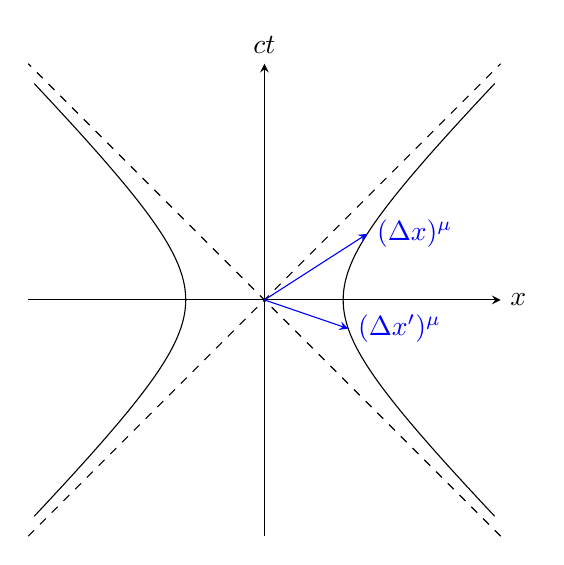
\begin{tikzpicture}
		\draw[-stealth] (-3, 0) -- (3, 0) node[right] {\( x \)};
		\draw[-stealth] (0, -3) -- (0, 3) node[above] {\( ct \)};
		\draw[dashed] (-3, -3 ) -- (3, 3);
		\draw[dashed] (3, -3) -- (-3, 3);
		\draw plot [variable = \t, samples=1000, domain=-70:70] 
			({1 / cos( \t )}, {1 * tan( \t )});
		\draw plot [variable = \t, samples=1000, domain=-70:70] 
			({-1 / cos( \t )}, {1 * tan( \t )});
		\draw[-stealth, blue] (0, 0) -- ({1 / cos(40)}, {1 * tan(40)})
			node[right] {\( (\Delta x)^{\mu} \)};
		\draw[-stealth, blue] (0, 0) -- ({1 / cos(-20)}, {1 * tan(-20)})
			node[right] {\( (\Delta x')^{\mu} \)};
	\end{tikzpicture}
\end{center}
Here, you can see that the hyperboloid is connected, so events can be Lorentz transformed into the past.  
This implies that for space-like events, there is no well defined causal structure. On the other hand, 
time-like events lie on a hyperboloid that is divided, so we do have a causal structure for time-like events. 

The transformations described up until now are denoted as \textit{active transformations}. They are
transformations that move the vector itself, while keeping the coordinate system fixed. On the contrary, we
can also imagine a \textit{passive} picture, where we alter the coordinate system instead of the vector
itself. To do this, we look back at the Lorentz transformation equations:
\[
	t' = \gamma\left( t - \frac{v}{c}x \right) \quad x' = \gamma(x - vt)
\]
Now, the \( x \)-axis corresponds to \( t = 0 \), so we have \( x' = \gamma x \). Likewise, the \( y \)-axis
corresponds to \( x = 0 \) so \( t' = \gamma t \). Therefore, our new axes transform to \( \gamma x \) and \(
\gamma t\):

\begin{center}
	\begin{tikzpicture}
		\draw[-stealth] (-3, 0) -- (3, 0) node[right] {\( x \)};
		\draw[-stealth] (0, -3) -- (0, 3) node[above] {\( ct \)};
		\draw[dashed] (-3, -3 ) -- (3, 3) node[above] {\( x = ct \)};
		\draw[dashed] (3, -3) -- (-3, 3);
		\draw[-stealth, orange] (0, 0) -- (3, 1) node[right] {\( x' \)};
		\draw[-stealth, orange] (0, 0) -- (1, 3) node[above] {\( ct' \)};
		\draw[orange] (1, 0) arc [start angle = 0, end angle = 9.46*2, radius = 1] node[midway, right] {\( \phi \)};
		% consider adding grid lines 
	\end{tikzpicture}
\end{center}
The angle \( \phi \) between the original and the altered axis is the same \( \phi \) we encountered earlier:
\( \phi = \tan^{-1}(v / c) \). In the passive picture, the event doesn't shift, but our axes and coordinate system
shifts to compensate. Just like the active frame though, this transformation allows for the breaking of
simultaneity, which you can show by tracing the grid line to the axis and figure out when that event occurs
in the boosted frame.  

\subsection{Dual Vectors}
Now, we come to the formal discussion of dual vectors. Remember from earlier, we denoted the spacetime
interval as \( ds^2 = \eta_{\mu \nu} x^{\mu}x^{\nu} \), where \( \eta \) is called the \textit{metric}. Then,
when we introduced 4-vectors, we introduced an inner product on them, defining it as \( \eta_{\mu \nu
}V^{\mu}W^{\nu} \). One way to think about this inner product is as presented, where we slap an \( \eta_{\mu
\nu} \) wherever we need it. Another way we think about it is through the context of dual vectors, by reading
the notation as \( (\eta_{\mu \nu}V^{\mu}) W^{\nu} \). Here, \( \eta_{\mu \nu}V^{\mu} \) is now a new object
which we will call a \textit{dual vector}, which we will define as \( V_{\nu} \equiv \eta_{\mu \nu}V^{\mu}
\).  

Now, notice what happens when we transform a vector into a dual vector. Suppose we start with the standard
vector \( V^{\mu} = \begin{pmatrix} V^{0} & V^{1} & V^{2} & V^{3} \end{pmatrix} \), and we now consider its
dual:
\[
	V_{\mu} = \eta_{\mu \nu}V^{\nu} = \begin{pmatrix} \eta_{0 \nu}V^{\nu} & \eta_{1 \nu} V^{\nu} & \eta_{2
		\nu} V^{\nu} & \eta_{3 \nu}V^{\nu}  \end{pmatrix} = \begin{pmatrix} -V^{0} & V^{1} & V^2 & V^3 \end{pmatrix}
\]
So compared to \( V^{\mu} \), the dual \( V_{\mu} \) has its time direction reversed. This has implications
for how the dual vector transforms, since we ultimately still want the dot product to be invariant. To see
how the dual transforms, we will have to set up some machinery first. Define the inverse matrix \( \eta^{\mu
\nu} \) such that \( \eta^{\mu \nu} \eta_{\nu \rho} = \delta^{\mu}_\rho \). Ironically enough, the explicit
form of \( \eta^{\mu \nu} \) actually looks the same as \( \eta_{\mu \nu} \):
\[
	\eta^{\mu \nu} = \begin{pmatrix} -1 &  & & \\ & 1 & & \\ & & 1 & \\ && & 1 \end{pmatrix}
\]
but it should be understood as a different object entirely. 

\begin{aside}
	Now that we're dealing with upper and lower indices, now's a good time to talk about why we never really
	cared about the ordering of the indices when taking a dot product. It's because they are in fact equal:
	\[
		\eta_{\mu \nu} V^{\mu}W^{\nu} = V_{\nu}W^{\nu} = V_\nu(\eta_{\nu \rho} W_{\rho}) = V^{\rho}W_{\rho}
	\]
\end{aside}
Now, recall that \( \Lambda \) satisfies \( \eta_{\mu \nu} \Lambda^{\mu}_\rho \Lambda^{\nu}_{\sigma} =
\eta_{\rho \sigma} \). Now, we multiply on the right by \( (\Lambda^{-1})^{\sigma}_\lambda \), and simplify
it:
\begin{align*}
	\eta_{\mu \nu}\Lambda^{\mu}_{\rho}\Lambda^{\nu}_\sigma \left( \Lambda^{-1} \right)^{\sigma}_\lambda &=
	\eta_{\rho \sigma}\left( \Lambda^{-1} \right)^{\sigma}_\lambda\\
	\eta_{\mu \nu}\Lambda^{\mu}_\rho \delta^{\nu}_\lambda &= \eta_{\rho \sigma}
	\left(\Lambda^{-1}\right)^{\sigma}_\lambda\\
	\eta_{\mu \lambda} \Lambda^{\mu}_\rho &= \eta_{\rho \sigma}\left( \Lambda^{-1} \right)^{\sigma}_\lambda 
\end{align*}
Now, we \textit{define} \( \Lambda_{\lambda \rho} \equiv \eta_{\mu \lambda}\Lambda^{\mu}_\rho \), which gives
us the relation:
\begin{equation}
	\Lambda_{\lambda \rho} = \left( \Lambda^{-1} \right)_{\rho \lambda}
\end{equation}
This equation can roughly be interpreted as saying that the inverse of \( \Lambda \) is its transpose. Now
with \( \Lambda^{-1} \) introduced, how does \( V_{\mu} \) transform under a Lorentz transformation? 
\begin{align*}
	V'_{\mu} = \eta_{\mu \nu}V'^{\nu} &= \eta_{\mu \nu} \Lambda^{\nu}_\rho V^{\rho}\\
	&= \Lambda_{\mu \rho}V^{\rho} \\ 
	&= \left( \Lambda^{-1} \right)_{\rho \nu} V^{\rho} \\ 
	&= \left( \Lambda^{-1} \right)^{\rho}_\nu V_\rho
\end{align*}
So in contrast with \( V^{\mu} \), the dual \( V_{\mu} \) uses the inverse \( \Lambda^{-1} \) to transform.
This way, the dot product:
\begin{align*}
	V^{\mu}W_{\mu} \to V'^{\mu}W'_{\mu} &= \left( \Lambda^{\mu}_\rho V^{\rho} \right)\left( \left(
	\Lambda^{-1} \right)^{\lambda}_\mu W_\lambda \right)\\
	&= \left( \Lambda^{-1} \right)^{\lambda}_\mu \Lambda^{\mu}_\rho V^{\rho}W_\lambda \\ 
	&= \delta^{\lambda}_\rho V^{\rho}W_\lambda \\ 
	&= V^{\lambda}W_\lambda 
\end{align*}
Hence the invariance of the dot product is preserved.  
 

 







	\section{April 30}
\subsection{4-Velocity}
Earlier, we saw that \( \tilde u = \dv{x^{\mu}}{t} \) is not a valid 4-vector, as it does not transform like
\( x^{\mu} \) under Lorentz transforms.
A better alternative is to use the proper time instead: \( u^{\mu} = \dv{x^{\mu}}{\tau} \). 
This is guaranteed to be a valid 4-vector, since the numerator is a
4-vector and the proper time is Lorentz invariant. Thus, \( U^{\mu} \) transforms as \( U^{\mu} \to
\Lambda^{\mu}_\nu V^{\nu} \).

In component form, \( u \) can be written as:
\[
	u = \begin{pmatrix} c \dv{t}{\tau} \\ \dv{x^{i}}{\tau} \end{pmatrix} = \begin{pmatrix} \gamma c \\
\dv{t}{\tau} \dv{x^{i}}{\tau} \end{pmatrix} = \begin{pmatrix} \gamma c \\ \gamma v \end{pmatrix}
\]
Now here's the trick with 4-velocity: if we move together with the particle, then our relative speed with it
will be zero, so the 4-velocity vector is:
\[
	u^{\mu} = \begin{pmatrix} c \\ \mathbf{0} \end{pmatrix}
\]
Now, if we take the dot product \( U^{\mu}U_{\mu} = \eta_{\mu \nu}U^{\mu}U^{\nu} = \eta_{00} U^{0}U^{0} =
-c^2 \). But using the property that the dot product is Lorentz invariant, it means that the inner product \(
U^{\mu}U_{\mu} = -c^2\)	in \textit{all} frames, even when the velocity vector is not zero! This gives us an
important rule to remember when calculating dot products: we want to always choose a frame in which it is
easiest to calculate dot products, and leverage Lorentz invariance. 

\subsection{4-Momentum}
With the 4-velocity defined, it is then natural to define also the 4-momentum: \( P^{\mu} = m U^{\mu} \).
This is particularly a natural form to choose since it is a natural extension of our classical momentum \( p
= mv \). Like 4-velocity, we need to ensure that momentum is conserved, so we want the 4-momentum to also
behave as a 4-vector -- this is easy to guarantee since we've already established \( U^{\mu} \) as a
4-vector. 

The fact that \( P^{\mu} \) transforms linearly under Lorentz transformations actually guarantees
conservation of momentum! To see this, consider a collision between two particles, that generates two other
ones:
\begin{center}
	\begin{tikzpicture}
		\draw[-stealth] (-1, 1) node[left] {\( 1 \)} -- (0, 0.5);
		\draw[-stealth] (-1, -1) node[left] {\( 2 \)} -- (0, -0.5);
		\draw[-stealth] (1, 0.5) -- (2, 1) node[right] {\( 3 \)};
		\draw[-stealth] (1, -0.5) -- (2, -1) node[right] {\( 4 \)};
	\end{tikzpicture}
\end{center}
Suppose in the \( \mathcal{S} \) frame, the 4-momentum \( P_1^{\mu} + P_2^{\mu} = P_3^{\mu} + P_4^{\mu} \).
Then, in the \( \mathcal{S}' \) frame, we have:
\[
	P_1' + P_2' = \Lambda(P_1) + \Lambda(P_2) = \Lambda(P_1 + P_2) = \Lambda(P_3 + P_4) = P_3' + P_4'
\]
so the momentum is automatically conserved! The explicit form of \( P^{\mu} \) is more or less the 
same as \( U^{\mu} \):
\[
	P^{\mu} = \begin{pmatrix} mv^{0} \\ m U^{i} \end{pmatrix} = \begin{pmatrix} \gamma mc \\ \gamma
	m \mathbf{v} \end{pmatrix} = \begin{pmatrix} E / c \\ \mathbf{p} \end{pmatrix}
\]
Here, we define \( E = \gamma mc^2 \) to be the relativistic energy and \( \mathbf{p} = \gamma mv \) to be
the relativistic momentum. Notice how naturally these formulas come out simply from our constraint that we
want our vectors to transform linearly under the Lorentz transform; hopefully this gives more insight into
how these formulas came to be, and that they're not as contrived as they appear to be in your introductory
classes. 

Now's also a good place to note that when \( v \ll c \), the classical formulas come out. When \(  v\ll c \),
then \( \gamma \approx 1 \), so \( \mathbf{p} \approx m \mathbf{v} \). Likewise, if we Taylor expand \( E \):
\[
	E = \left( 1 + \frac{1}{2} \frac{v^2}{c^2} \right) mc^2 = mc^2 + \frac{1}{2}mv^2
\]
the first term represents the rest mass energy and is the formula \( E = mc^2 \), and the second term 
is exactly the kinetic energy term we're all familiar with. 

We can also write the speed of a particle in terms of \( E \) and \( \mathbf{p} \):
\[
	\frac{pc}{E} = \frac{\gamma mv c}{\gamma mc^2} = \frac{v}{c} \implies v = \frac{pc^2}{E}
\]
Another thing: if we take \( p_{\mu}p^{\mu} \):
\[
	p_{\mu}p^{\mu} = \eta_{\mu \nu}p^{\mu}p^{\nu} = -\frac{E^2}{c^2} + |\mathbf{p}|^2
\]
On the other hand, we know that since \( p^{\mu} = m U^{\mu} \), then the inner product is also equal to:
\[
	p_{\mu}p^{\mu} = m U_{\mu}(m U^{\mu}) = m^2 U_{\mu}U^{\mu} = -m^2 c^2
\]	
So we can combine these two equations together:
\begin{equation}
	\label{relativistic-energy}
	-\frac{E^2}{c^2} + |\mathbf{p}|^2 = -m^2 c^2 \implies E^2 = |\mathbf{p}|^2 c^2 + m^2 c^{4}
\end{equation}
this should also be a familiar equation. One property about this equation is that because it is a result of
equating two dot products, this identity is \textit{Lorentz invariant}, and holds true for any object in any
frame. 

So far, the above equations for particles with mass, but without mass, what happens? Well,
\cref{relativistic-energy} tells us that when \( m = 0 \), then \( E = |\mathbf{p}|c \), so its velocity:
\[
	v = \frac{pc^2}{pc} = c
\]
so massless particles travel at the speed of light!   

\subsection{4-Forces}
With 4-momentum established, it is now natural for us to go even further, and generalize forces into a
4-vector. We call this \( f^{\mu} \), which we will define as:
\[
	f^{\mu} = \dv{p^{\mu}}{\tau}
\]
again, as a classical generalization of Newton's second law \( F = \dv{p}{t} \). In component form:
\[
	\dv{p^{\mu}}{\tau} = \begin{pmatrix} \frac{1}{c} \dv{E}{\tau} \\ \dv{\mathbf{p}}{\tau} \end{pmatrix} =
\begin{pmatrix} \frac{1}{c} \dv{t}{\tau} \dv{E}{t} \\ \dv{t}{\tau} \dv{\mathbf{p}}{\tau} \end{pmatrix} = 
\begin{pmatrix} \frac{\gamma}{c} \dv{E}{t} \\ \gamma \dv{\mathbf{p}}{t} \end{pmatrix}
\]
If there is no 4-force acting on our particle, then we expect that \( \dv{p^{\mu}}{\tau} = 0 \), which is the
equation of motion of a free particle.

\subsection{Action of Free Relativistic Particles}
According to the stationary action principle, the evolution of any physical system should be one such that
the action is stationary. That is, we require \( \delta S = 0 \). Note that we only require the derivative to
be zero, not that it is minimized or maximized.\footnote{The Lagrangian is always convex, so we can always
guarantee minima or maxima, there won't be any "saddle points".} According to special relativity, because
physics should behave the same in all inertial frames, then the action should also be Lorentz invariant. 

When a particle travels through space, the path it traces out is called its \textbf{worldline}. Because it
describes how the particle moves, a natural candidate for the action would be the spacetime interval of its
worldline:
\[
	S_\text{particle} = -mc \int dS
\]
here we have a prefactor of \( mc \) for historical reasons, we don't need to care about these prefactors
very much. If we now parametrize our action by \( \lambda \), then the action may be written as:
\[
	S_\text{particle} = -mc \int \sqrt{\eta_{\mu \nu} \dv{x^{\mu}}{\lambda} \dv{x^{\nu}}{\lambda}} \diff\lambda
\]
Then, when we vary the action using \( x^{\mu}(\lambda) \to x^{\mu} + \delta x^{\mu} \), then we have:
\begin{align*}
	\delta S &= -mc \int \delta\sqrt{-\eta_{\rho \sigma} \dv{x^{\rho}}{\lambda} \dv{x^{\sigma}}{\lambda}}
	\diff \lambda \\ 
			 &= -mc \int \frac{\delta\left( -\eta_{\mu \nu} \dv{x^{\mu}}{\lambda} \dv{x^{\nu}}{\lambda}
			 \right)}{2 \sqrt{-\eta_{\rho \sigma} \dv{x^{\rho}}{\lambda} \dv{x^{\sigma}}{\lambda}}} \\ 
			 &= -mc \int \frac{-2 \eta_{\mu \nu} \dv{x^{\mu}}{\lambda} \dv{(\delta x^{\nu})}{\lambda}}{2
			 \sqrt{-\eta_{\rho \sigma} \dv{x^{\rho}}{\lambda} \dv{x^{\sigma}}{\lambda}}} 
\end{align*}
Now we do integration by parts, which means we slap a differential around everything but the \( \dv{(\delta
x^{\nu}}{\lambda} \) term, giving us:
\[
	\delta S = mc \int \dv{\lambda} \left( \frac{\eta_{\mu \nu} \dv{x^{\mu}}{\lambda}}{\sqrt{-\eta_{\rho
	\sigma} \dv{x^{\rho}}{\lambda} \dv{x^{\sigma}}{\lambda}}} \right) \delta x^{\nu}
\]
If we then require that \( \delta S = 0 \) for any \( \delta x^{\nu} \), then the requirement is that
everything else must equal to zero:
\[
	-mc \left( \frac{\eta_{\mu \nu} \dv{x^{\mu}}{\lambda}}{\sqrt{-\eta_{\rho \sigma} 
	\dv{x^{\rho}}{\lambda} \dv{x^{\sigma}}{\lambda}}} \right) = 0
\]
This equation may look ugly at first, but it is only written as such because we haven't specified how we want
to parametrize the worldline. If we choose a simple parametrization like the proper time (i.e. \( \lambda =
\tau \)), then we get:
\[
	-mc \dv{\tau} \left( \frac{\eta_{\mu \nu} \dv{x^{\mu}}{\tau}}{\sqrt{-\eta_{\rho \sigma}
	U^{\rho}U^{\sigma}}} \right) = -m \dv{p_{\nu}}{\tau} = 0 \implies \dv{p_{\mu}}{\tau} = 0
\]
so what comes out is a very natural equation: the statement that the net force on a free particle is zero.  
 





 















	\section{May 2}

\subsection{Natural Units}
In this lecture, we should mention that from here on out we will be using natural units, where \( c = \hbar = 1
\). This is so that we don't have to carry the constants everywhere we go, and it also has some beneifts in
the way of dimensional analysis. In particular, since \( c = 1 \), then the dimension for length is the same
as time:
\[
	[L] = [T]
\]
which is particularly natural especially in relativity since length and time can be interchanged with each
other. Setting \( \hbar = 1 \), which usually carries the units of \( [E][T] \), means that we now regard
energy and time as inverses:
\[
	[E] = [T]^{-1}
\]
From \( E = mc^2 \), because \( c = 1 \), then this implies that \( [E] = [M] \) and combining this with the
previous relations we get the big chain:
\[
	[L] = [T] = [E]^{-1} = [M]^{-1}
\]
\subsection{Action of a Free scalar field}
Consider a scalar field \( \phi = \phi(x) = \phi(t, \mathbf{x}) \). Our goal is to find an action that
satisfies the three criteria:
\begin{enumerate}[label=\arabic*.]
	\item Quadratic in \( \phi \). We want this because we want the equations of motion to be linear in \(
		\phi \), and hence we want the action to be quadratic in \( \phi \). 
	\item Lorentz invariant. We want this because the action gives us the equations of motion, through the
		stationary action principle, and obviously we want them to be the same in all inertial frames.   
	\item Involve \( \partial_\mu \phi \). We want this because we want a time evolution \( \dot \phi \)
		term. We don't want to just use \( \partial_t \phi \) since in relativity time and space are
		interchangeable, so we use the general derivative \( \partial_\mu \phi \) instead. 
\end{enumerate}

It turns out, the action that satisfies these three is:
\[
	S = -\frac{1}{2}\int d^{4}x \left[ \eta^{\mu \nu}\partial_\mu \phi \partial_\nu \phi + m^2 \phi^2 \right]
\]
In natural units, \( S \) should be dimensionless, and you can check that the right hand side has units of \(
[E][T] \) so the equation is correct. Now, just like any other action, we first vary the field by introducing
\( \phi(x) \to \phi(x) + \delta \phi(x) \): 
\[
	\delta S = -\frac{1}{2}\int d^{4}x \, \delta \left[ \eta^{\mu \nu}\partial_\mu \phi \partial_\nu \phi 
	+ m^2 \phi^2 \right] = -\frac{1}{2}\int d^{4}x  \, \left[ 2 \eta^{\mu \nu} \partial_\mu \phi
	\, \delta(\partial_\nu \phi) + 2m^2 \phi\,  \delta \phi \right]
\]
Now, in the first term the variation of the derivative, \( \delta(\partial_\nu \phi) \) can be written as:
\[
	\delta (\partial_\nu \phi) = \partial_\nu (\phi + \delta \phi) - \partial_\nu \phi = \partial_\nu (\delta
	\phi)
\]
So we can write the entire integral as:
\[
	- \int d^{4}x \, \left[ \partial_\nu \left( \eta^{\mu \nu}\partial_\mu \phi \partial_\nu \phi \right) -
	\partial_\nu \left( \eta^{\mu \nu} \partial_\nu \phi \right) \delta \phi + m^2 \phi \, \delta \phi \right]
\]
Now we will take integration by parts. We will assume that we only vary the field locally, so at the extremes
\( \delta \phi = 0 \), allowing us to drop the boundary term. So, this gives us:
\[
	\int d^{4} x \, \left[ \eta^{\mu \nu} \partial_\mu \partial_\nu \phi - m^2 \phi \right] \delta \phi
\]
If we require \( \delta S = 0 \) for any variation in the field, then the term in square brackets must be
zero. Removing the index notation, the equation reads:
\[
	(-\partial_t^2 + \nabla^2 - m^2) \phi = 0
\]
This is known as the \textbf{Klein-Gordon Equation}. Notice that it looks like a wave equation, except it
has a mass term. The other thing of note is that this equation is linear in \( \phi \), 
which explains why we wanted our action that is quadratic in \( \phi \) from earlier. 
If we had more higher order terms in the action, then they'd contribute
to the right hand side effectively acting as source terms just like how they appeared in the wave equations
for the fields \( V \) and \( \mathbf{A} \).   

For equations of motion without a source, then our solutions are plane waves:
\[
	\phi = A e^{i(Et - \mathbf{p} \cdot \mathbf{x})} = Ae^{-i p^{\mu}p_{\mu}}
\]
Substituting this back into the equation, we get:
\[
	(E^2 - |\mathbf{p}|^2 - m^2) A e^{i (Et - \mathbf{p} \cdot \mathbf{x})} = 0 \implies E^2 - |\mathbf{p}|^2
	- m^2 = 0
\]
This is exactly the relativistic equation for energy: \( E^2 = p^2 c^2 + m^2 c^{4} \). 

\subsection{Action of Massless 4-Vector Fields}
The above section takes care of scalar fields, but as we've studied in electromagnetism, the electric and
magnetic fields are vector fields, so this section will be dedicated to writing its action and the resulting
equations of motion. As we will see, Maxwell's equations will come right out at the end. 

We will consider a "free" field at first, then add source terms later. Because we are working in a
relativistic context, we should use the 4-vector field \( A^{\mu} \) instead of the standard 3-vector. This
allows us to impose the following conditions:
\begin{enumerate}[label=\arabic*.]
	\item Quadratic in \( A_\mu \) because we want an equation of motion that is linear in \( A_\mu \).    
	\item Lorentz invariance. We want Lorentz invariance here for the same reason as the scalar field.  
	\item Need to involve \( \partial_\nu A_\nu \), just like we involved \( \partial_\mu \phi \) from
		before. 
	\item The action should be massless. We want this in particular because we want to match
		electromagnetism, which has no mass terms. As such, we will drop the \( \frac{1}{2}m^2 A^{\mu}A_\mu
		\) term from the action.  
\end{enumerate}
So what kind of action can we write? If we want Lorentz invariance, that also satisfies the third condition,
then one thing we can do is write something like:
\[
	(\partial_\rho A_\sigma) (\partial_\mu A_\nu)
\]
but we can't just leave it as is, since the action must be dimensionless. So, we need to find a way to
contract these indices, of which there are two ways:
\begin{enumerate}[label=\arabic*.]
	\item \( (\partial^{\mu}A^{\nu})(\partial_\mu A_\nu) \)
	\item \( (\partial_\mu A^{\mu})(\partial_\nu A^{\nu}) \)
\end{enumerate}
Note there is a third way \( A^{\mu}(\partial^2 A_\mu) \), but if we expand this out:
\[
	A^{\mu}(\partial^2 A_\mu) = A^{\mu}(\partial^{\nu} \partial_\nu A_\mu) = \partial^{\nu}(A^{\mu}
	\partial_\nu A_\mu) - (\partial^{\nu} A^{\mu})(\partial_\nu A_\mu)
\]
We've now written this in the form of a total derivative term and the same equation as in method 1. Because
we eventually get rid of total derivative terms anyways, this way of contracting ends up being the same as
the first, so there are really only two unique ways to contract these indices. Our action can now be written
as a combination of the two ways:
\[
	S = -\frac{1}{2}\int d^{4}x \, \left[ a \left( \partial_\mu A_\nu \right)\left( \partial^{\mu}A^{\nu}
	\right) + b \left( \partial_\mu A^{\mu} \right) \left( \partial_\nu A^{\nu} \right) \right]
\]
Now, we vary the action:
\[
	\delta S = -\frac{1}{2}\int d^{4}x \, \left[ a (\partial_\mu A_\nu) \delta(\partial^{\mu}A^{\nu}) + b
	(\partial_\mu A^{\mu}) \delta(\partial_\nu A^{\nu}) \right] 
\]
Now we do integration by parts and remove the total derivative:
\begin{align*}
	\delta S &= \int d^{4}x \, \left[ a \partial^{\mu} (\partial_\mu A_\nu) \delta A^{\nu} + b
	\partial_\nu(\partial_\mu A^{\mu}) \delta A^{\nu} \right] \\ 
	&= \int d^{4}x \, \left[ a \partial^{\mu}\partial_\mu A_\nu + b \partial_\nu \left( \partial_\mu A^{\mu}
	\right) \right] \delta A^{\nu} 
\end{align*}
Now, requiring that \( \delta S = 0 \) for any \( \delta A^{\nu} \) means we get:
\[
	\partial^{\mu} \partial_\mu A_\nu + b \partial_\nu (\partial_\mu A^{\mu}) = 0
\]
The free equation of motion is then (we raised the free index \( \nu \) here, it does nothing except makes
the equation a bit nicer to look at):
\[
	a \partial^{\mu} \partial_\mu A^{\nu} + b \partial^{\nu}(\partial_\mu A^{\mu}) = 0
\]
So this is the free equation. Now, we want to add the effect of sources, which we will do by adding them to
the right side of this equation. Because the left hand side is a 4-vector, then the thing we add on the right
must also be a 4-vector:
\begin{equation}
	\label{vector-action}
	a \partial^{\mu} \partial_\mu A^{\nu} + b \partial^{\nu} (\partial_\mu A^{\mu}) = J^{\nu}
\end{equation}
Adding \( J^{\nu} \) here is analogous to what we had with the Lorentz gauge back in chapter 10: 
\begin{align*}
	(\partial_t^2 - \nabla^2) \phi &= \rho\\
	(\partial_t^2 - \nabla^2) \mathbf{A} &= \mathbf{J}
\end{align*}
where terms like the charge and current density can be regarded as "sources".  We will also require \( J^{\nu} \)
to be conserved, such that:
\[
	\partial_\nu J^{\nu} = 0
\]
One way to argue that we need this constraint is to think about charges and currents: we want these
quantities to be conserves, so its generalized version \( J^{\nu} \) should also be conserved. The above
equation for conservation also has a nice meaning if we allow \( J^{\nu} = (\rho, \mathbf{J}) \) when we
expand out the summation notation:
\[
	\partial_t \rho + \nabla \cdot \mathbf{J} = 0
\]
this is the standard continuity equation! Hopefully this small demonstration shows why we need this constraint, and
that it is indeed a well-motivated result. Now, for consistency, if we take \( \partial_\nu \) of both sides
of \cref{vector-action}:
\[
	\partial_\nu \left( a \partial^{\mu}\partial_\mu A^{\nu} + b \partial^{\nu}\left( \partial_\mu A^{\mu}
	\right) \right) = \partial_\nu J^{\nu} = 0
\]
So this gives us the relation:
\[
	a \partial^2 (\partial_\nu A^{\nu}) + b \partial^2 (\partial_\mu A^{\mu}) = 0
\]
both terms here \( \partial_\nu A^{\nu} \) and \( \partial_\mu A^{\mu} \) are of the same form, so the only
combination of \( a, b \) that makes this zero is \( a = -b \). By convention, we will let \( a = 1 \) and \(
b = -1\). So in summary, the action with the conserved current reads:
\[
	S = -\frac{1}{2}\int d^{4} \, \left( \partial_\mu A_\nu \partial^{\mu} A^{\nu} - (\partial_\mu A^{\mu})
	(\partial_\nu A^{\nu}) \right) + \int d^{4}x \, A_\mu J^{\mu}
\]
Now, we define \( F_{\mu \nu} \equiv \partial_\mu A_\nu - \partial_\nu A_\mu \). Then, \( F^{\mu \nu} F_{\mu
\nu} \) gives:
\begin{align*}
	F^{\mu \nu} F_{\mu \nu} &= \left( \partial_\mu A_\nu - \partial_\nu A_\mu \right)\left(
	\partial^{\mu}A^{\nu} - \partial^{\nu} A^{\mu} \right)\\
	&= 2(\partial_\mu A_\nu)(\partial^{\mu}A^{\nu}) - 2(\partial_\nu A_\mu)(\partial^{\nu}A^{\mu}) \\ 
	&= 2(\partial_\mu A_\nu) (\partial^{\mu}A^{\nu}) - 2(\partial^{\mu}A_\mu) (\partial_\nu A^{\nu}) 
\end{align*}
This is exactly twice the first integral, so we can rewrite the action as:
\[
	S = -\frac{1}{4}\int d^{4}x \, F_{\mu \nu} F^{\mu \nu} + \int d^{4}x \, A_\mu J^{\mu}
\]
Now, forcing \( \delta S = 0 \) eventually gets us:\footnote{we skipped the algebra in class in the interest
of time.}
\begin{equation}
	\label{maxwell-1}
	\partial_\mu F^{\mu \nu} = J^{\mu}
\end{equation}
In addition, because of the antisymmetry of \( F^{\mu \nu} \) (which you can see from its definition), we
have the relation:
\begin{equation}
	\label{maxwell-2}
	\partial_\lambda F_{\mu \nu} + \partial_\nu F_{\lambda \mu} + \partial_\mu F_{\nu \lambda} = 0
\end{equation}
As it turns out, \cref{maxwell-1,maxwell-2} are exactly Maxwell's equations in index notation! In particular,
\cref{maxwell-1} gives Gauss's and the Ampere-Maxwell law, since these two equations deal with source terms.
The other two are given by \cref{maxwell-2}. To see this worked out 
explicitly, let \( A^{\mu} = (V, \mathbf{A}) \) and \( A_\mu = (-V, \mathbf{A}) \), then from
\cref{maxwell-1} we have:
\begin{align}
	\label{f0i}F_{0i} &= \partial_0 A_i - \partial_i A_0 = \partial_t A_i - \partial_i V = \partial_t A_i - \nabla V =
	E_i\\
	\label{fij}F_{ij} &= \partial_i A_j - \partial_j A_i = \epsilon_{ijk}B^{k}
\end{align}
So, putting \cref{f0i} into \cref{maxwell-1} gives us:
\[
	\partial_0 F^{00} + \partial_i F^{0i} = \rho \implies \partial_i E_i = \nabla \cdot \mathbf{E} = \rho
\]
Working this out with the other indices gives you Ampere-Maxwell too. For \cref{maxwell-2}, if you let \(
\lambda \mu \nu = 0ij \) and iterate, then you get:
\[
	\partial_0 F_{ij} + \partial_j F_{0i} + \partial_{i}F_{i0}
\]
Then, using \cref{f0i,fij}, then this becomes:
\[
	-\partial_t \left( \epsilon_{ijk}B^{k} \right) + \partial_j E_i - \partial_i E_j = 0
\]
Contracting with \( \epsilon^{ijm} \epsilon_{ijk} \), then this becomes:
\[
	-2 \partial_t B^{m} - \epsilon^{ijm}\left( \partial_i E_j - \partial_j E_i \right)	
\]
Finally, \( \partial_i E_j - \partial_j E_i = 2 \partial_i E_j \), so we indeed get Faraday's law:
\[
	\nabla \times \mathbf{E} = -\partial_t \mathbf{B}
\]
likewise, \( \nabla \cdot \mathbf{B} = 0 \) follows as well from the other indices. And that concludes our
derivation of Maxwell's equations! It's nice that we've essentially come full circle from the beginning: we
started with Maxwell's equations, and finished by deriving them. What is truly remarkable is that these
equations naturally fall out as a result of our two constraints on the action and the current, where neither
of them directly reference the equations at all -- they are simply a product of these two constraints. If
that's not beautiful, I don't know what is. 
 
 

\end{document}
